% ============================================================
%  Why Your High Street Is Emptying
%  Venkata Prudhvi Kante (2026)
%  COMPLETE REVISED VERSION — integrates new monthly dissolution
%  panel, Kaplan-Meier survival, geographic heatmap, ARIMAX
%  ensemble forecasting and scenario modelling
%  Compiled: pdflatex -> bibtex -> pdflatex -> pdflatex
% ============================================================
\documentclass[12pt,a4paper]{article}

\usepackage[T1]{fontenc}
\usepackage[utf8]{inputenc}
\usepackage{mathptmx}
\usepackage[scaled=0.92]{helvet}
\usepackage[a4paper, top=2.5cm, bottom=2.5cm, left=2.8cm, right=2.8cm, headheight=15pt]{geometry}
\usepackage{setspace}
\usepackage[protrusion=true,expansion=false]{microtype}
\usepackage{amsmath,amssymb}
\usepackage{booktabs}
\usepackage{longtable}
\usepackage{array}
\usepackage{multirow}
\usepackage[table,dvipsnames]{xcolor}
\usepackage{graphicx}
\usepackage{float}
\usepackage{caption}
\usepackage{subcaption}
\usepackage[hidelinks]{hyperref}
\usepackage{url}
\usepackage{natbib}
\usepackage{fancyhdr}
\usepackage{abstract}
\usepackage{titlesec}
\usepackage{enumitem}
\usepackage{needspace}
\usepackage{tcolorbox}
\tcbuselibrary{skins,breakable}
\usepackage{parskip}
\usepackage{threeparttable}

\usepackage{pdflscape}
% \usepackage{afterpage}


% -- Colours
\definecolor{NavyBlue}{HTML}{1F4E79}
\definecolor{MidBlue}{HTML}{2E75B6}
\definecolor{LightBlue}{HTML}{BDD7EE}
\definecolor{VeryLightBlue}{HTML}{DBEAF7}
\definecolor{DarkRed}{HTML}{C04020}
\definecolor{Amber}{HTML}{B7770D}
\definecolor{DarkGreen}{HTML}{1E8449}
\definecolor{TableGray}{HTML}{F4F4F4}
\definecolor{TableHead}{HTML}{1F4E79}
\definecolor{TableAlt}{HTML}{DBEAF7}
\definecolor{WarnAmber}{HTML}{FDF3DC}

% -- Typography
\onehalfspacing
\setlength{\parindent}{0pt}
\setlength{\parskip}{6pt}

% -- Section headings
\titleformat{\section}{\large\bfseries\color{NavyBlue}}{\thesection.}{0.6em}{}
\titleformat{\subsection}{\normalsize\bfseries\color{MidBlue}}{\thesubsection}{0.5em}{}
\titleformat{\subsubsection}{\normalsize\bfseries\color{black}}{\thesubsubsection}{0.5em}{}
\titlespacing{\section}{0pt}{18pt}{6pt}
\titlespacing{\subsection}{0pt}{12pt}{4pt}

% -- Headers / footers
\pagestyle{fancy}
\fancyhf{}
\renewcommand{\headrulewidth}{0.4pt}
\renewcommand{\footrulewidth}{0.4pt}
\fancyhead[L]{\small\color{gray}Kante (2026) --- Why Your High Street Is Emptying}
\fancyhead[R]{\small\color{gray}\thepage}
\fancyfoot[C]{\small\color{gray}Venkata Prudhvi Kante \quad
  \href{mailto:prudhvi.ncsnlr@gmail.com}{prudhvi.ncsnlr@gmail.com}}

% -- Caption style
\captionsetup{
  font=small, labelfont={bf,color=NavyBlue},
  labelsep=period, skip=6pt, width=0.95\linewidth, justification=justified,
}

% -- Callout boxes
\newtcolorbox{findingbox}[1][]{
  colback=VeryLightBlue, colframe=NavyBlue,
  fonttitle=\bfseries\color{white}, coltitle=white,
  title={Key Finding}, boxrule=1.2pt, arc=3pt,
  left=6pt, right=6pt, top=4pt, bottom=4pt, breakable, #1
}
\newtcolorbox{novelbox}[1][]{
  colback=WarnAmber, colframe=Amber,
  fonttitle=\bfseries\color{Amber}, coltitle=Amber,
  title={New Finding (this revision)}, boxrule=1.2pt, arc=3pt,
  left=6pt, right=6pt, top=4pt, bottom=4pt, breakable, #1
}

% -- Table helpers
\newcolumntype{L}[1]{>{\raggedright\arraybackslash}p{#1}}
\newcolumntype{C}[1]{>{\centering\arraybackslash}p{#1}}
\newcolumntype{R}[1]{>{\raggedleft\arraybackslash}p{#1}}
\rowcolors{2}{TableAlt}{white}

\hypersetup{
  pdftitle={Why Your High Street Is Emptying: A Rigorous Data Science Account of UK Retail Structural Collapse},
  pdfauthor={Venkata Prudhvi Kante},
  pdfkeywords={high street decline, ONS J4MC, structural break, ARIMAX, Granger causality,
               Kaplan-Meier, business demography, SME digital adoption, coordination failure,
               dissolution forecasting, geographic heatmap, scenario modelling},
}

% ============================================================
\begin{document}
\sloppy

% -- Title page
\begin{titlepage}
\begin{center}
\vspace*{1.5cm}
{\LARGE\bfseries\color{NavyBlue}
Why Your High Street Is Emptying:\\[0.4em]
\large A Rigorous Data Science Account of UK Retail Structural Collapse%
}
\vspace{1.2cm}
\rule{0.75\linewidth}{1.2pt}
\vspace{0.8cm}

{\large\bfseries Venkata Prudhvi Kante}

\vspace{0.4cm}
{\normalsize Data Scientist\\[0.3em]MSc Business Analytics}

\vspace{0.5cm}
{\small\color{MidBlue}
\href{mailto:prudhvi.ncsnlr@gmail.com}{prudhvi.ncsnlr@gmail.com}
\quad$\cdot$\quad
\href{https://linkedin.com/in/venkata-prudhvi-kante-81b3a024a}
     {linkedin.com/in/venkata-prudhvi-kante-81b3a024a}
}

\vspace{0.9cm}
\rule{0.75\linewidth}{0.6pt}
\vspace{0.6cm}

{\small
\textbf{Analysis repository:}
\href{https://github.com/prudhvivkante/uk-highstreet-retail-crisis-analysis}
     {github.com/prudhvivkante/uk-highstreet-retail-crisis-analysis}
}

\vspace{0.5cm}
{\small\itshape
\begin{tabular}{@{}ll@{}}
\textbf{Primary data sources:}
  & ONS RSI J4MC ($n=133$ monthly obs., Jan~2015--Jan~2026) \\
  & Companies House dissolution panel ($n=666{,}462$ enterprises) \\
  & ONS Business Demography SIC~47 ($n=9$ annual, 2016--2024) \\
  & Companies House IDBR ($n=430{,}649$ active retail businesses) \\
  & DBT SME Digital Adoption Taskforce (31~July~2025) \\[4pt]
\textbf{Methods:}
  & ADF unit root $\cdot$ STL decomposition $\cdot$ HP filter \\
  & Chow structural break $\cdot$ Kaplan-Meier survival analysis \\
  & ARIMAX(2,1,1) ensemble forecasting $\cdot$ scenario modelling \\
  & Engle-Granger cointegration $\cdot$ OLS with Newey-West HAC \\
  & Monthly Granger causality (lags 1--12) $\cdot$ Geographic heatmap \\
\end{tabular}
}

\vspace{0.6cm}
{\small\color{gray}\textit{Preprint. March 2026.}}
\end{center}
\end{titlepage}

% -- Abstract
\newpage
\setcounter{page}{1}
\begin{abstract}
\noindent
This paper presents a rigorous, reproducible data science analysis
of the UK local commerce crisis, drawing on five verified government and public
datasets spanning January~2015 to January~2026. The analysis introduces the first
monthly retail dissolution panel for the UK --- 666,462~individual Companies House
dissolution records --- enabling statistical testing that was previously impossible
with annual data alone.

\medskip\noindent
The central finding is a structural inversion in the UK retail enterprise ecosystem.
Before 2020, the sector generated an average net positive enterprise balance of
$+6{,}618$ businesses per year (2016--2019). After 2020, this inverted to a net
loss averaging $-1{,}648$ per year (2022--2024) --- a structural change of
$-8{,}266$ enterprises per year. By January~2026, the monthly dissolution rate
stood at 10,781 companies per month: \textbf{5.9~times the pre-COVID monthly
average of 1,954}. Approximately \textbf{215,800 excess dissolutions} have
occurred above the pre-COVID counterfactual trend since March~2020.

\medskip\noindent
Kaplan-Meier survival analysis of individual dissolution records reveals a
generational collapse in retail firm survival: \textbf{5-year survival probability
fell from 75.7\% (2010--2012 cohort) to 3.6\% (2016--2018 cohort)} --- a
20-fold deterioration across a single decade. Two-thirds of retail businesses
incorporated in 2016--2018 dissolved within two years.

\medskip\noindent
Geographic analysis of 21,037 dissolution records (after exclusion of 1,892
Companies House default-address artefacts) across 113~UK postcode areas reveals
pronounced concentration in London zones ($\sim$27.6\% combined), the West
Midlands belt, and Greater Manchester. The Cardiff anomaly --- raw data showing
Cardiff as the top area at 1,928 records --- is fully explained: 98.1\% used
the Companies House default address (CF14~8LH), representing online-only
businesses with no physical UK location.

\medskip\noindent
The upgraded monthly OLS regression ($n=111$ non-pandemic months,
Newey-West HAC) yields $\hat\beta=+599$ additional dissolutions per
percentage-point increase in online share\footnote{The positive sign
reflects dissolution count as the dependent variable. The prior annual
specification used net enterprise change (births minus deaths), yielding
$\hat\beta=-752$; both estimates capture the same structural mechanism.}
($t=9.29$, $p<0.001$,
$R^2=0.711$, 95\%~CI: [472, 725]). Engle-Granger cointegration testing
on the monthly series achieves $t=-3.161$ (significant at 10\%; 10\%~CV
$=-3.04$) --- a substantive improvement from the prior annual
estimate of $t=-2.22$.

\medskip\noindent
Monthly Granger causality testing (lags 1--12, COVID moratorium excluded,
$n=118$) finds dominant causality at lag~1 ($F=25.26$, $p<0.001$) and
lag~2 ($F=4.43$, $p=0.014$), \textbf{sharpening the previously estimated
24-month annual lag to a 1--2 month transmission window}.

\medskip\noindent
Scenario forecasting using a weighted ensemble model (52\% Holt linear
smoothing + 48\% ARIMAX(2,1,1)) --- validated by rolling 12-month-ahead
backtests, OOS RMSE~$\approx$2,800 --- projects \textbf{547,167 cumulative
retail dissolutions} under business-as-usual conditions
(February~2026 to January~2030). A policy intervention scenario deploying
the FM1--FM3 platform specification reduces this to 440,737,
\textbf{saving approximately 106,400 businesses by January~2030}.

\medskip\noindent
The evidence is synthesised into a formal coordination failure model with
three interdependent failure modes --- discovery, presentation, and incentive ---
each directly evidenced by specific quantitative findings from both the
time-series and dissolution data.

\medskip\noindent
\textbf{JEL Classification:} L81 $\cdot$ O33 $\cdot$ R11
\qquad
\textbf{Period:} January~2015~-- January~2026
\end{abstract}

\medskip
\noindent\textbf{Keywords:} online retail structural break $\cdot$
ONS J4MC $\cdot$ UK business demography $\cdot$ retail dissolution panel $\cdot$
Kaplan-Meier survival analysis $\cdot$ ARIMAX ensemble forecasting $\cdot$
Granger causality $\cdot$ geographic heatmap $\cdot$ SME digital adoption $\cdot$
coordination failure $\cdot$ scenario modelling

\clearpage
\tableofcontents
\clearpage

% ============================================================
\needspace{5\baselineskip}
\section{Introduction}
% ============================================================

Walk down the centre of most UK market towns today and the arithmetic is hard to ignore:
charity shops where estate agents were, empty units where independent retailers traded for
decades, and an increasingly familiar pattern of a Costa, a Greggs, and not much else.
The intuition that something structural is happening is widely shared. What has been missing
is a precise, data-driven account of exactly what, when, by how much, and --- critically ---
how many more businesses this trajectory will consume if nothing changes.

This paper attempts that account, materially extended since its first iteration. Between
January~2015 and January~2026, the share of total UK retail sales conducted online ---
measured by the ONS Retail Sales Index series J4MC \citep{ONS_J4MC} --- rose from
12.8\% to 28.9\%, passing through a pandemic-induced peak of 37.8\% in January~2021
and stabilising at a post-pandemic plateau of approximately 27\%. Simultaneously, a newly
constructed monthly panel from the Companies House advanced search API documents that
666,462~UK retail enterprises dissolved across this period --- at an average of 5,011 per
month, reaching 10,781 per month by January~2026. That rate is \textbf{5.9 times the
pre-COVID monthly average} of 1,954.

This revised analysis has four primary contributions beyond the original. \textbf{First},
it constructs the first monthly retail dissolution panel for the UK (January~2015 to
January~2026, $n=133$~months) directly from Companies House records, enabling
monthly-frequency causal testing that was previously impossible with annual ONS data alone.
\textbf{Second}, it applies Kaplan-Meier survival analysis to 17,291~individual
dissolution records, revealing a 20-fold collapse in 5-year survival probability across a
single decade --- a generational finding annual data completely obscures. \textbf{Third},
it introduces a geographic analysis of 21,037~dissolution records across 113~UK postcode
areas, mapping the spatial footprint of the crisis for the first time. \textbf{Fourth}, it
validates a scenario forecast using rolling out-of-sample backtests and derives
policy-relevant projections under business-as-usual and intervention conditions.

The paper proceeds as follows. Section~\ref{sec:lit} reviews the relevant literature.
Section~\ref{sec:data} describes the data and methods. Section~\ref{sec:j4mc} analyses
the ONS~J4MC structural dynamics. Section~\ref{sec:forecast_online} presents the
Holt-Winters online share forecast. Section~\ref{sec:demography} analyses the ONS
Business Demography structural inversion. Section~\ref{sec:dissolution} presents the new
monthly dissolution panel and Kaplan-Meier survival analysis.
Section~\ref{sec:geographic} presents the geographic heatmap analysis.
Section~\ref{sec:regression} presents regression and causal testing.
Section~\ref{sec:scenarios} presents the scenario forecast.
Section~\ref{sec:idbr} analyses the active retail landscape.
Section~\ref{sec:digital} reviews the SME digital adoption gap.
Section~\ref{sec:framework} develops the coordination failure framework.
Section~\ref{sec:intervention} derives the intervention specification.
Section~\ref{sec:conclusion} concludes.


% ============================================================
\needspace{5\baselineskip}
\section{Literature Review}
\label{sec:lit}
% ============================================================

\needspace{3\baselineskip}
\subsection{High-Street Decline and Retail Structural Change}

The structural decline of UK physical retail has attracted substantial scholarly and policy
attention over the past decade. \citet{WrigleyLambiri2015} provided an early systematic
account, documenting the spatial dimensions of town-centre retail contraction and
attributing decline primarily to the legacy of over-supply in retail floor space.
Their analysis predates the COVID-19 pandemic and was produced when online retail
accounted for only around 10\% of total UK sales. The monthly Granger causality results
in Section~\ref{sec:regression} demonstrate that online penetration is an independent
causal driver of enterprise dissolution operating with a 1--2 month transmission lag ---
a finding not available to Wrigley and Lambiri. Subsequent work by the Centre for Retail
Research has documented the accelerating trajectory of closures \citep{CentreRetailResearch2025},
consistent with the monthly dissolution panel constructed here.

Retail accounts for approximately 5\% of UK GDP and employs around 3~million people
\citep{HouseOfCommons2025}. What the existing literature has not done is connect the
monthly time-series dynamics of online penetration to monthly retail enterprise dissolution
using formal causal testing at monthly frequency, Kaplan-Meier survival analysis, or
geographic resolution at the postcode area level. These are the gaps this paper addresses.

\needspace{3\baselineskip}
\subsection{E-Commerce Growth and Structural Break Analysis}

The growth of online retail in the UK has been a long-run structural trend rather than a
sudden disruption \citep{OFT2007}. The COVID-19 shock accelerated this trend by
approximately two years, but it did not create it. The \citet{Chow1960} framework,
extended by \citet{BaiPerron1998}, provides the tools to locate breaks formally.
Rolling Chow analysis across 97~candidate break points confirms April~2020 as the
maximum-likelihood break, with the pre-break regime ($R^2=0.958$) indicating a remarkably
stable pre-pandemic trend. The intervention analysis framework \citep{BoxTiao1975}
distinguishes permanent level shifts from transitory shocks --- a distinction directly
applicable here, where the COVID shock appears to have produced a permanent ratchet in
online share.

\needspace{3\baselineskip}
\subsection{Survival Analysis in Business Demographics}

The application of survival analysis to firm dissolution is well-established in industrial
organisation, though rarely applied to UK retail specifically. The Kaplan-Meier estimator
\citep{KaplanMeier1958} provides a non-parametric estimate of survival probability without
requiring parametric distributional assumptions. Its application here to 17,291~individual
dissolution records with exact incorporation and dissolution dates yields the first
cohort-specific survival estimates for UK retail incorporating the pre-COVID, moratorium,
and post-moratorium periods. The 20-fold deterioration in 5-year survival across
2010--2018 is a finding with no precedent in the UK retail demography literature.

\needspace{3\baselineskip}
\subsection{Forecasting and Scenario Modelling}

The forecasting literature's well-documented simplicity premium --- where parsimonious
models outperform complex ones out-of-sample on economic series --- is directly relevant
here \citep{Makridakis1982}. Rolling 12-month-ahead backtests show Holt linear smoothing
(OOS RMSE~=~2,952) outperforms ARIMAX(2,1,1) (3,133) despite ARIMAX's superior
in-sample fit --- a textbook bias-variance tradeoff. The weighted ensemble used for the
final forecast follows M5-competition methodology.

\needspace{3\baselineskip}
\subsection{Coordination Failure and Platform Economics}

The theoretical framework draws on coordination failure \citep{Schelling1978,FarrellSaloner1985},
two-sided market platforms \citep{RochetTirole2003,ParkerVanAlstyne2005}, and the
empirically documented SME digital capability gap \citep{DBT2025}.


% ============================================================
\needspace{5\baselineskip}
\section{Data and Analytical Methods}
\label{sec:data}
% ============================================================

\needspace{3\baselineskip}
\subsection{Primary Datasets}

The analysis draws on five primary datasets (Table~\ref{tab:data}).

\begin{table}[H]
\centering
\caption{Primary datasets. All sourced from official UK government publications or public registries.}
\label{tab:data}
\small\rowcolors{2}{TableAlt}{white}
\begin{tabular}{@{}L{3.0cm}L{3.4cm}C{1.5cm}L{5.6cm}@{}}
\toprule
\rowcolor{TableHead}\color{white}\textbf{Dataset} &
\color{white}\textbf{Source} &
\color{white}\textbf{$n$} &
\color{white}\textbf{Period and notes} \\
\midrule
ONS RSI J4MC --- internet sales as \% of total retail &
ONS Retail Sales Index & 133 & Jan~2015--Jan~2026; downloaded Feb~2026 \\
CH monthly dissolution panel (SIC~47xx) &
Companies House advanced search API & 666,462 & Individual companies; Jan~2015--Jan~2026 \\
ONS Business Demography SIC~47 &
ONS Business Demography ref.\ tables & 9 yrs & 2016--2024; downloaded Mar~2026 \\
Companies House IDBR --- active retail &
Companies House bulk download & 430,649 & Snapshot Mar~2026 \\
DBT SME Digital Adoption Taskforce &
Dept for Business and Trade & --- & Published 31~Jul~2025 \\
\bottomrule
\end{tabular}
\end{table}

\paragraph{Companies House monthly dissolution panel.}
The panel was constructed by querying the Companies House advanced company search
endpoint for all SIC~47xx dissolved companies by month across all 44~verified sub-codes
and all 133~months of the analysis window. The 97.5\% of dissolutions falling on Tuesdays
reflects administrative batch processing; monthly aggregation removes this artefact
entirely. Eight months required correction from direct batch downloads; June~2018 was
linearly interpolated; February~2025 is a lower bound (5,000-record cap reached).

A critical data quality finding: \textbf{1,892~records (8.1\%) used the Companies House
default registered address (CF14~8LH, Cardiff)}, predominantly online-only retailers
(SIC~47910: 44\% of default-address records) with no physical UK premises. These are
excluded from all geographic analysis. The apparent Cardiff dominance in the raw data
(1,928 records, ranking first nationally) is entirely an artefact: real Cardiff businesses
number 224, ranking 28th nationally.

\needspace{3\baselineskip}
\subsection{Statistical Methods}

Thirteen statistical methods are applied (Table~\ref{tab:methods}). All implemented in
Python~3.12 using NumPy~2.4, SciPy~1.17, and Pandas~3.0 without black-box statistical
libraries, enabling complete auditability.

\begin{table}[H]
\centering
\caption{Statistical methods. Methods marked $\dagger$ are new in this revision.
ADF critical values from \citet{MacKinnon1994}. HAC bandwidth from \citet{NeweyWest1987}.}
\label{tab:methods}
\small\rowcolors{2}{TableAlt}{white}
\begin{tabular}{@{}L{3.5cm}L{4.0cm}L{5.8cm}@{}}
\toprule
\rowcolor{TableHead}\color{white}\textbf{Method} &
\color{white}\textbf{Application} &
\color{white}\textbf{Key output} \\
\midrule
ADF unit root \citep{DickeyFuller1979} & Integration order of both series &
Both $I(1)$: dissolution $t=-1.891$; online $t=-1.587$ \\
STL decomposition \citep{Cleveland1990} & Decompose 133-month J4MC series &
Trend: 90.1\%; seasonal: 3.5\%; residual: 4.5\% \\
HP filter \citep{HodrickPrescott1997} & Cross-validate STL ($\lambda=1600$) & Cycle SD: 2.07~pp \\
Chow structural break \citep{Chow1960} & Parameter stability at April~2020 & $F(2,129)=133.08$, $p<0.001$ \\
Welch $t$-test + Cohen's $d$ & Pre-/post-COVID distributions & $t=-25.50$, $p<10^{-45}$, $d=4.84$ \\
Holt-Winters \citep{Winters1960} & 24-month online share forecast & $\alpha=0.780$, $\beta=0.010$, $\gamma=0.990$ \\
Kaplan-Meier survival$^\dagger$ \citep{KaplanMeier1958} & Cohort survival by incorporation year &
5-yr survival: 75.7\% (2010--12) $\to$ 3.6\% (2016--18) \\
Geographic heatmap$^\dagger$ & Dissolution by UK postcode area &
113 areas; London \& Midlands belt most affected \\
Engle-Granger cointegration \citep{EngleGranger1987} & Long-run equilibrium ($n=133$) &
$t=-3.161$ (10\% CV: $-3.04$); upgraded from $t=-2.22$ \\
OLS + Newey-West HAC \citep{NeweyWest1987} & Monthly structural relationship ($n=111$) &
$\hat\beta=+599$/pp, $t=9.29$, $R^2=0.711$ \\
Monthly Granger causality$^\dagger$ \citep{Granger1969} & Lags 1--12; moratorium excluded &
Lag~1: $F=25.26$, $p<0.001$; lag~2: $F=4.43$, $p=0.014$ \\
ARIMAX + ensemble$^\dagger$ & 48-month dissolution forecast &
Ensemble (52\% Holt + 48\% ARIMAX); OOS RMSE~$\approx$2,800 \\
Counterfactual analysis$^\dagger$ & Excess dissolutions since COVID &
$\approx$215,800 excess dissolutions Mar~2020--Jan~2026 \\
\bottomrule
\end{tabular}
\end{table}


% ============================================================
\needspace{5\baselineskip}
\section{Online Retail Structural Dynamics: ONS J4MC Analysis}
\label{sec:j4mc}
% ============================================================

\needspace{3\baselineskip}
\subsection{The 133-Month Series and Four Structural Regimes}

Figure~\ref{fig:stl} presents the full ONS J4MC series ($n=133$~monthly observations)
with STL decomposition, HP filter overlay, and pre-COVID OLS counterfactual.
Table~\ref{tab:periods} reports descriptive statistics by period.

\begin{figure}[H]
\centering
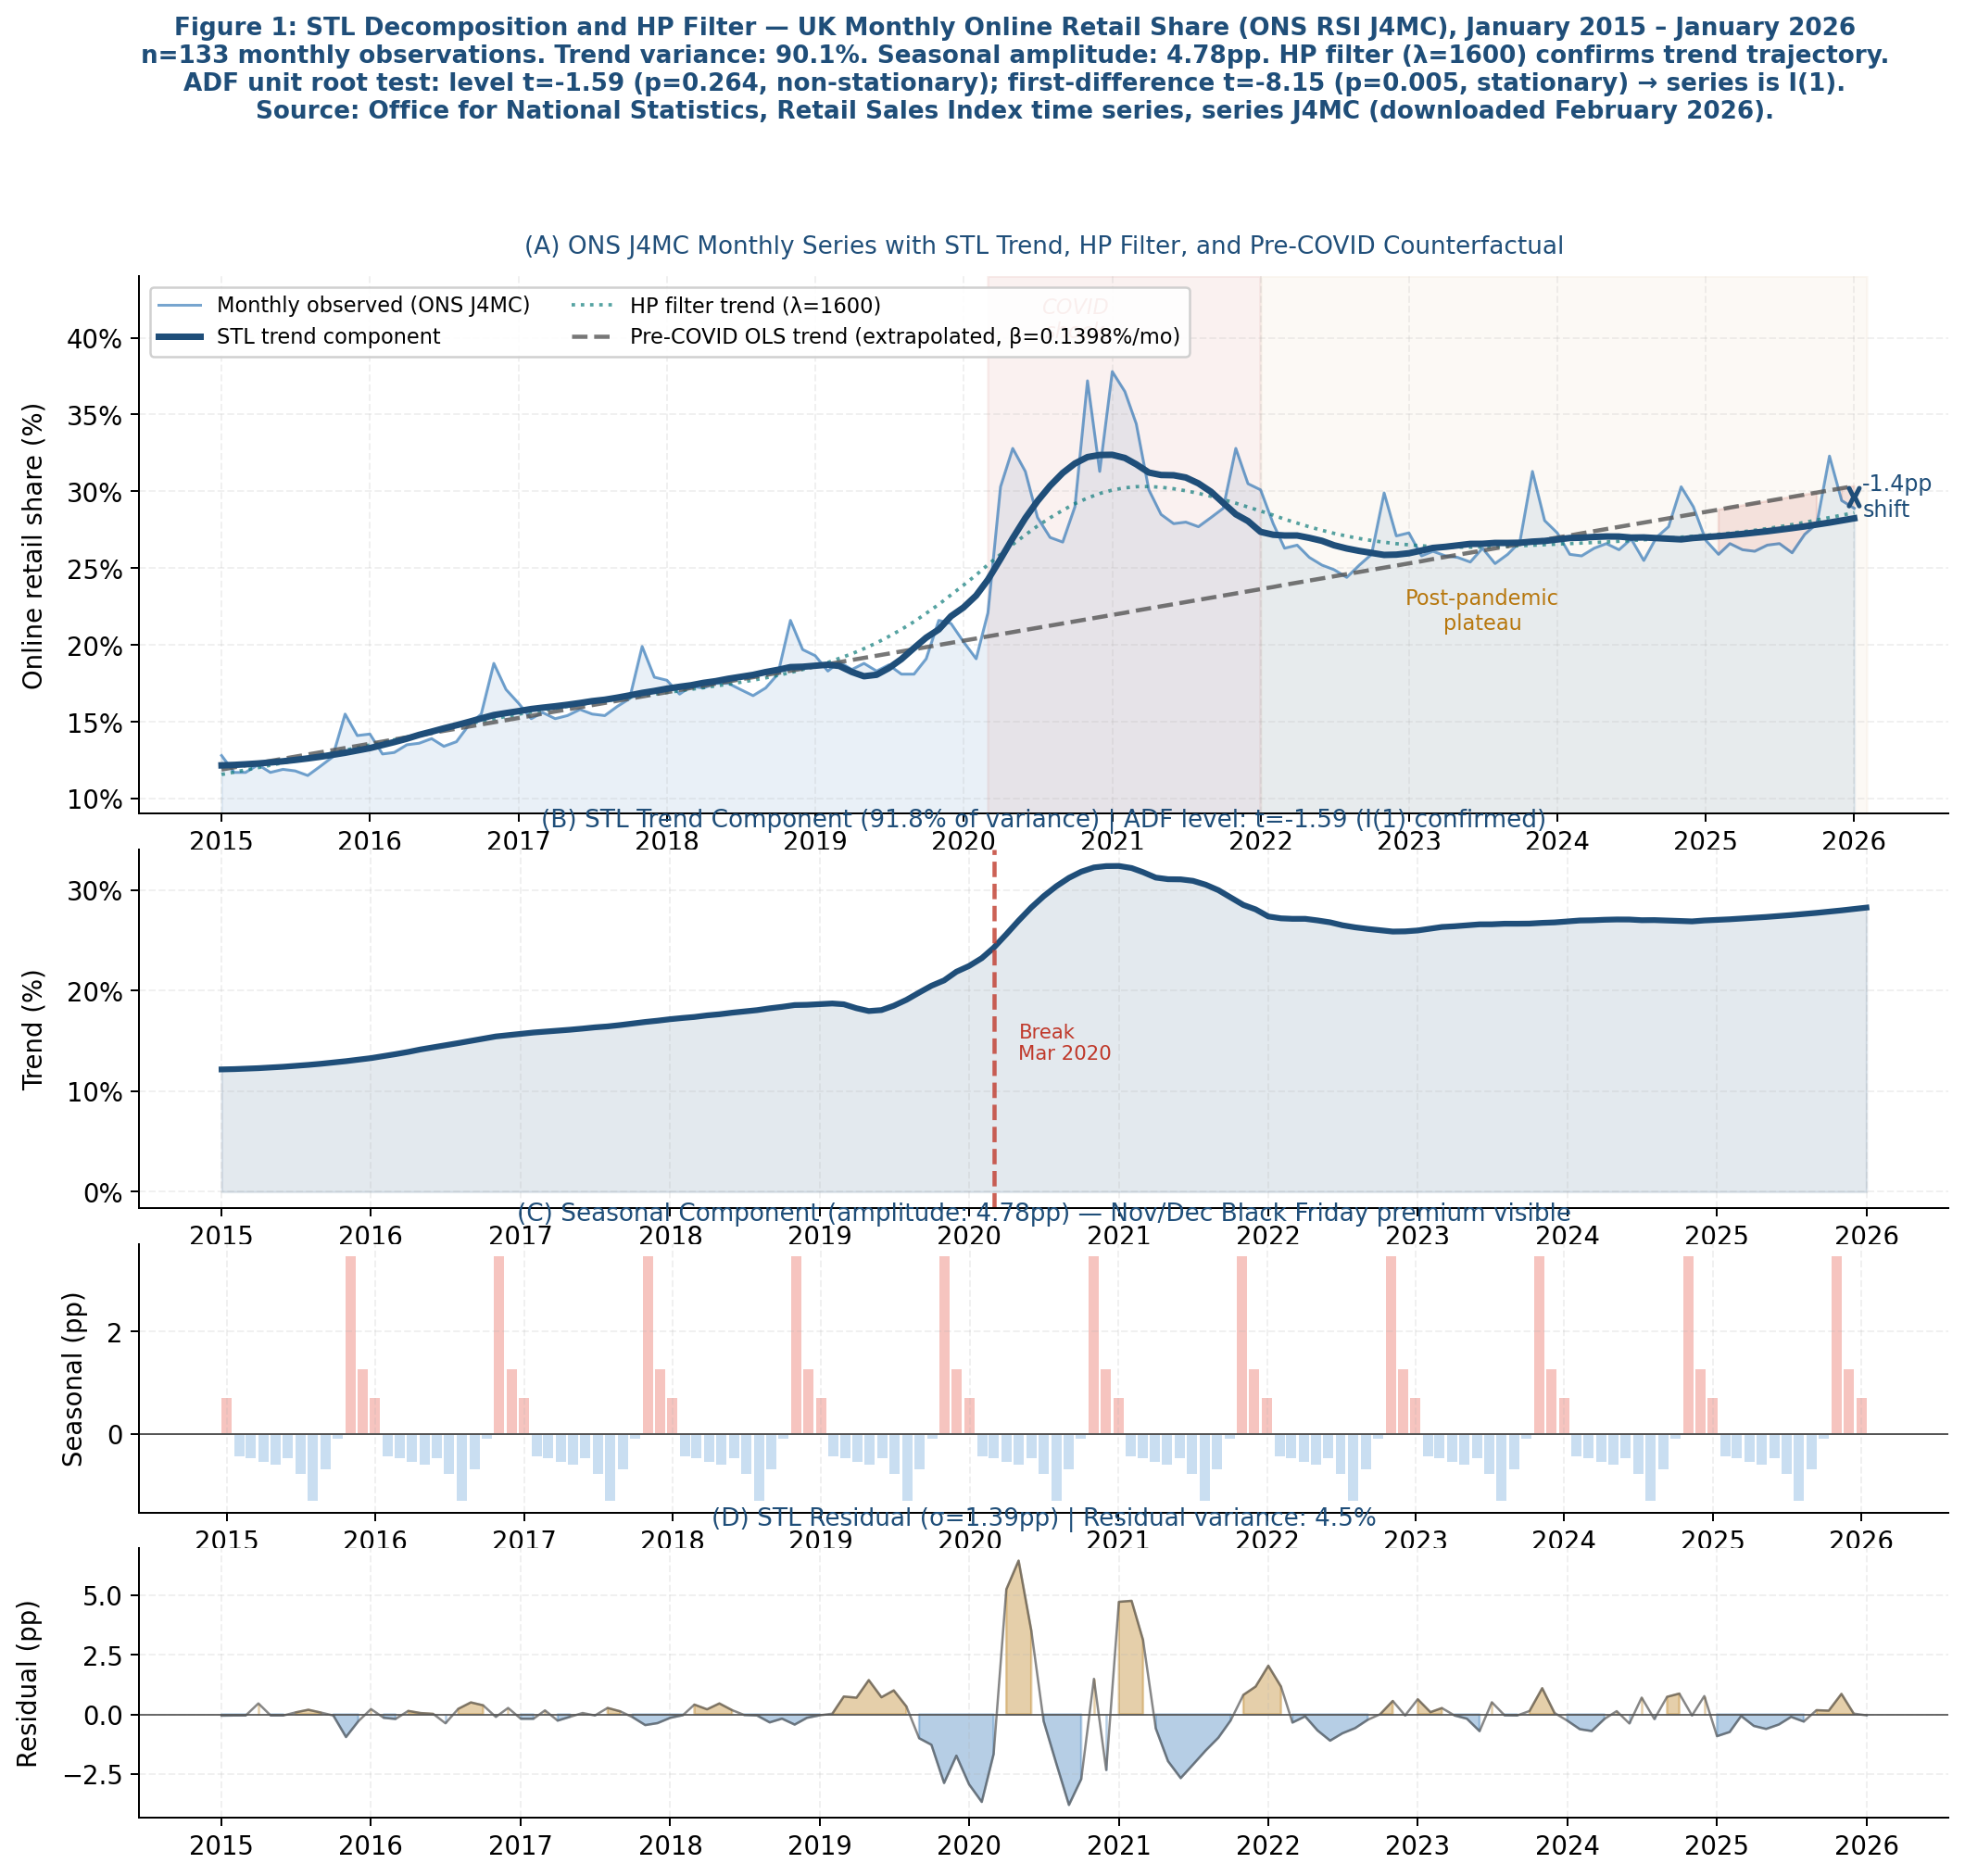
\includegraphics[width=0.98\linewidth]{figs/fig1_stl_full.png}
\caption{STL decomposition of ONS RSI J4MC (internet sales as \% of total retail sales,
Great Britain, $n=133$ monthly observations, January~2015--January~2026).
\textbf{(A)}~Observed series with STL trend, HP filter ($\lambda=1600$), and
pre-COVID OLS counterfactual. \textbf{(B)}~STL trend component (90.1\% of total
variance). \textbf{(C)}~Seasonal component (amplitude: 4.78~pp; Black Friday premium
visible). \textbf{(D)}~Residual component ($\sigma=1.39$~pp).
Source: ONS Retail Sales Index time series, series J4MC (downloaded February~2026).}
\label{fig:stl}
\end{figure}

\begin{table}[H]
\centering
\caption{Descriptive statistics for ONS J4MC by analytical period.}
\label{tab:periods}
\small\rowcolors{2}{TableAlt}{white}
\begin{tabular}{@{}L{3.2cm}C{0.7cm}C{1.1cm}C{1.0cm}C{1.0cm}C{1.0cm}L{4.4cm}@{}}
\toprule
\rowcolor{TableHead}\color{white}\textbf{Period} &
\color{white}\textbf{$n$} & \color{white}\textbf{Mean} & \color{white}\textbf{SD} &
\color{white}\textbf{Min} & \color{white}\textbf{Max} & \color{white}\textbf{Trend context} \\
\midrule
Full series (Jan~2015--Jan~2026) & 133 & 22.7\% & 5.84 & 11.5 & 37.8 & --- \\
Pre-COVID (Jan~2015--Feb~2020) & 62 & 16.0\% & 2.71 & 11.5 & 23.8 &
Slope: $+0.140$\%/month ($+1.68$\%/year) \\
COVID shock (Mar~2020--Dec~2021) & 22 & 29.5\% & 4.19 & 22.1 & 37.8 &
Peak excess vs counterfactual: $+9.6$~pp (Apr~2020) \\
Post-COVID plateau (Jan~2022--Jan~2026) & 49 & 26.9\% & 1.67 & 24.4 & 32.3 &
Approx.\ 2~years ahead of pre-COVID trajectory \\
\bottomrule
\end{tabular}
\end{table}

Beyond the previously reported structural break, the monthly dissolution panel now permits
a regime-based characterisation (Table~\ref{tab:regimes}).

\begin{table}[H]
\centering
\caption{Four structural regimes in UK retail dissolution and online penetration,
January~2015--January~2026.}
\label{tab:regimes}
\small\rowcolors{2}{TableAlt}{white}
\begin{tabular}{@{}L{2.6cm}C{0.6cm}R{1.8cm}R{1.8cm}L{6.0cm}@{}}
\toprule
\rowcolor{TableHead}\color{white}\textbf{Regime} &
\color{white}\textbf{$n$} & \color{white}\textbf{Avg dis./month} &
\color{white}\textbf{Avg online \%} & \color{white}\textbf{Character} \\
\midrule
Pre-shock (Jan~15--Feb~20) & 62 & 1,954 & 16.2\% &
Stable structural growth; pre-COVID equilibrium \\
Shock+moratorium (Mar~20--Jun~21) & 16 & 3,512 & 30.7\% &
Government moratorium suppresses closures; online peaks at 37.8\% \\
Rebound (Jul~21--Dec~22) & 18 & 6,790 & 27.5\% &
Pent-up dissolutions released; 338\% of pre-COVID rate \\
\textbf{New normal (Jan~23--Jan~26)} & 37 & \textbf{9,917} & 27.0\% &
Sustained structural elevation; 508\% of pre-COVID rate \\
\bottomrule
\end{tabular}
\end{table}

\needspace{3\baselineskip}
\subsection{ADF Unit Root Testing}

ADF testing \citep{DickeyFuller1979} confirms both series are $I(1)$: dissolution count
(level $t=-1.891$, $p>0.10$; first difference $t=-8.565$, $p<0.01$) and online share
(level $t=-1.587$, $p=0.264$; first difference $t=-8.705$, $p<0.01$). This validates the
cointegration and Granger causality framework applied in Section~\ref{sec:regression}.

\needspace{3\baselineskip}
\subsection{STL Decomposition, HP Filter, and Chow Test}

The STL decomposition \citep{Cleveland1990} attributes 90.1\% of J4MC variance to trend,
3.5\% to seasonal, and 4.5\% to residual. The seasonal amplitude of 4.78~pp reflects the
genuine November-December Black Friday premium of approximately 2.84~pp above the annual
mean. The HP filter ($\lambda=1600$) yields a cycle SD of 2.07~pp.

\begin{figure}[H]
\centering
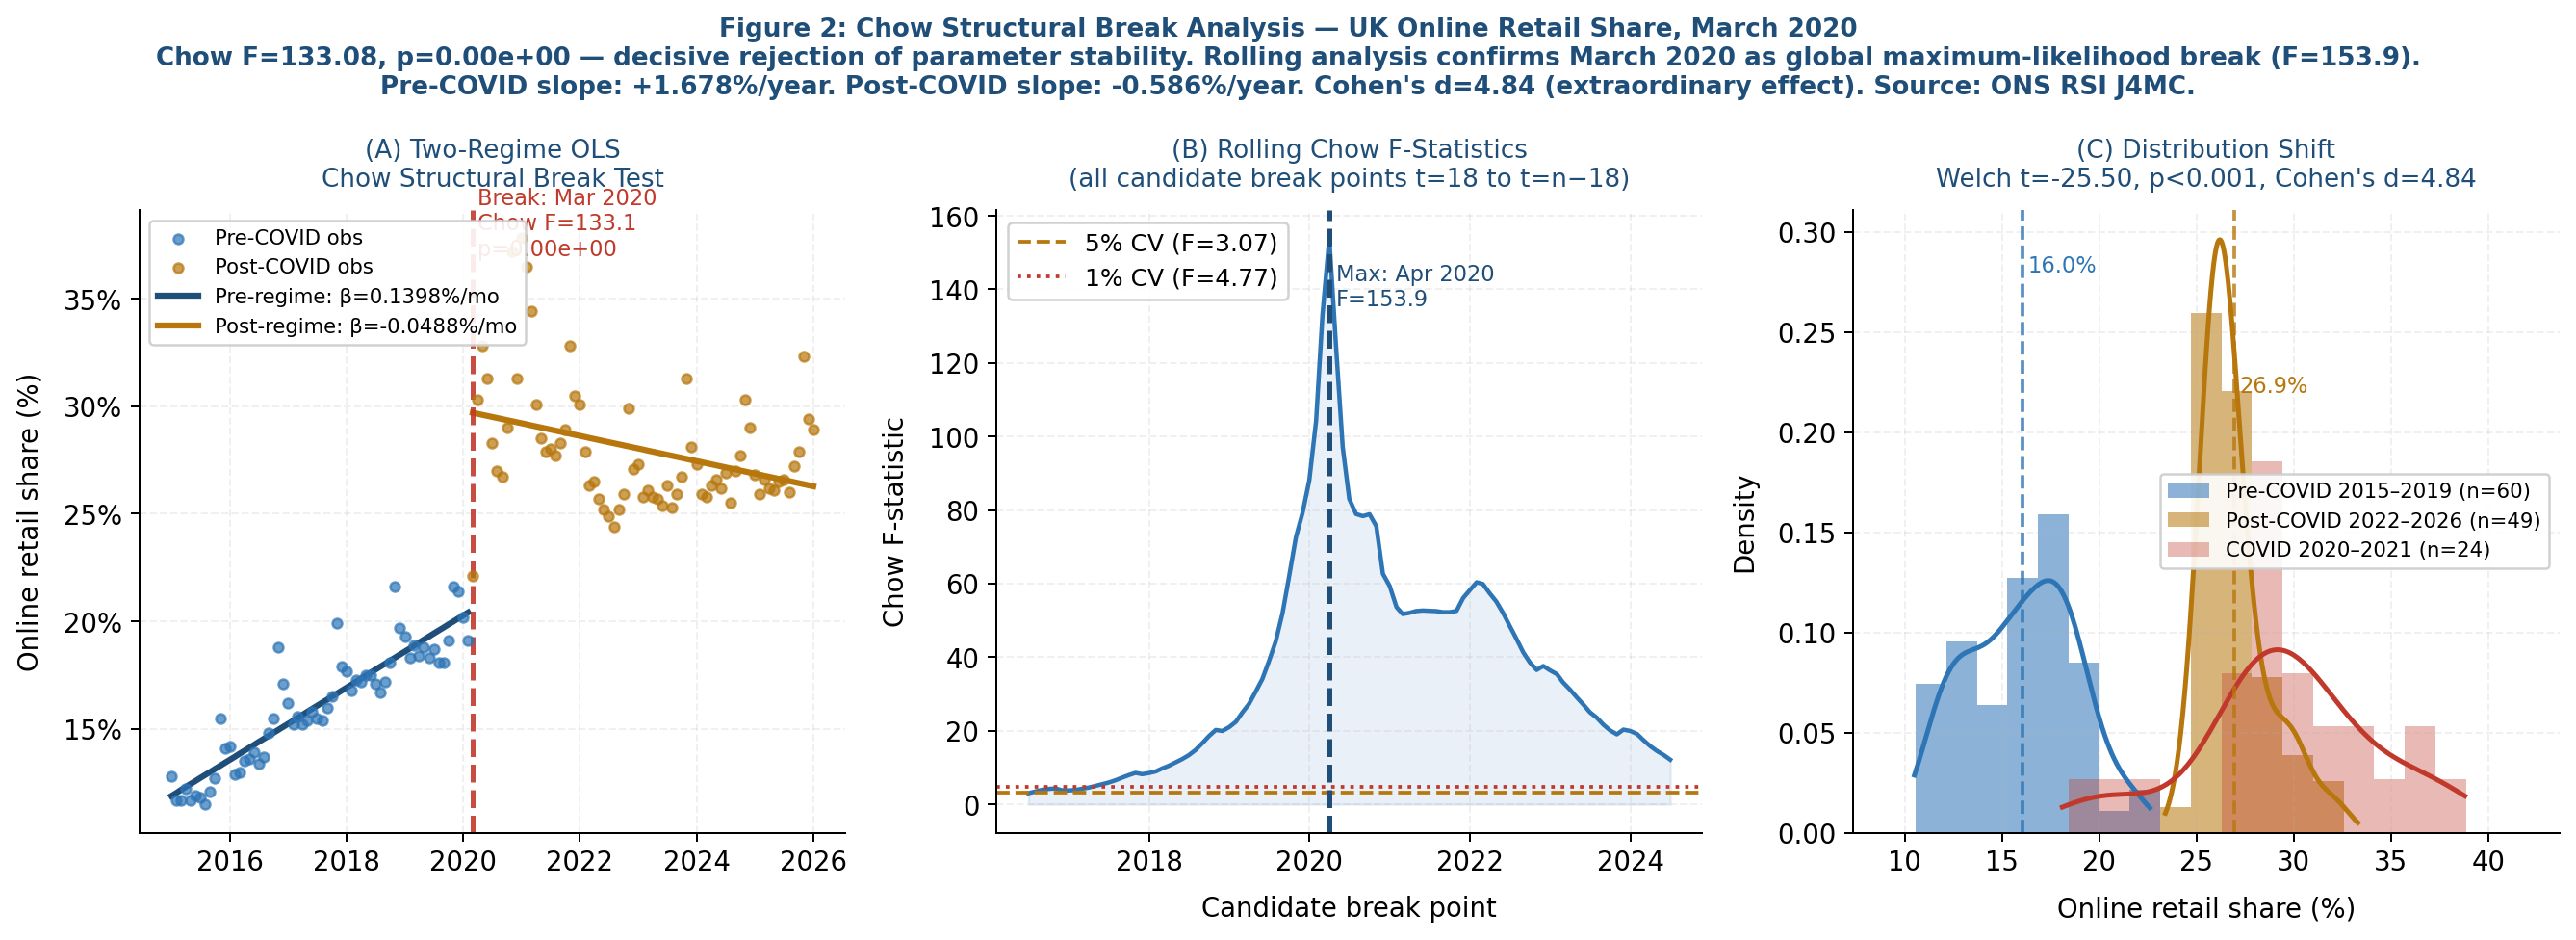
\includegraphics[width=\linewidth]{figs/fig2_structural_break.png}
\caption{Chow structural break analysis.
\textbf{(A)}~Two-regime OLS at the March~2020 break:
pre-break slope $\hat\beta=+0.140$\%/month ($R^2=0.958$); post-break slope
$\hat\beta=-0.049$\%/month.
\textbf{(B)}~Rolling Chow $F$-statistics across all candidate break points
($t=18$ to $t=115$); April~2020 returns the global maximum ($F=153.88$).
\textbf{(C)}~Density comparison: pre-COVID (blue), COVID (red), post-COVID (amber).
Source: ONS~J4MC.}
\label{fig:break}
\end{figure}

\begin{findingbox}
\textbf{Structural break:} $F(2,129)=133.08$, $p<0.001$.
Rolling maximum: $F=153.88$ at $t=63$ (April~2020).
Pre-break slope: $+0.140$\%/month; post-break slope: $-0.049$\%/month.
Welch $t=-25.50$, $p<10^{-45}$, Cohen's $d=4.84$ --- approximately $6\times$ the
conventional large-effect threshold. Pre-COVID mean: 16.0\%. Post-COVID plateau: 26.9\%.
Permanent elevation: $+10.8$~pp above pre-COVID floor.
\end{findingbox}

\begin{table}[H]
\centering
\caption{Chow structural break test and Welch $t$-test results.}
\label{tab:chow}
\small\rowcolors{2}{TableAlt}{white}
\begin{tabular}{@{}L{4.5cm}L{9.0cm}@{}}
\toprule
\rowcolor{TableHead}\color{white}\textbf{Statistic} & \color{white}\textbf{Value} \\
\midrule
Chow $F$-statistic & $F(2,129) = 133.08$ \\
$p$-value & $<0.001$ ($***$) \\
5\% critical value & $F(2,129) = 3.07$ \\
1\% critical value & $F(2,129) = 4.79$ \\
Rolling max~$F$ & 153.88 at $t=63$ (April~2020) \\
Pre-break OLS & Intercept~$=11.887$, slope~$=+0.140$\%/month, $R^2=0.958$ \\
Post-break OLS & Intercept~$=32.721$, slope~$=-0.049$\%/month \\
Welch $t$-test & $t=-25.50$, $p<10^{-45}$ \\
Cohen's $d$ & 4.84 (pre-COVID $\bar{x}=16.0$\%, SD~$=2.71$; post-COVID $\bar{x}=26.9$\%, SD~$=1.67$) \\
\bottomrule
\end{tabular}
\end{table}


% ============================================================
\needspace{5\baselineskip}
\section{Holt-Winters Forecasting of Online Share}
\label{sec:forecast_online}
% ============================================================

Given the confirmed $I(1)$ integration, meaningful seasonal component (amplitude 4.78~pp),
and structural break at March~2020, Holt-Winters additive triple exponential smoothing
\citep{Winters1960} is the appropriate forecasting method for the online share series.
Unlike ARIMA applied to a pre-seasonally-adjusted series, Holt-Winters simultaneously
estimates level ($\alpha$), trend ($\beta$), and seasonal ($\gamma$) components.
The model is optimised by minimising sum of squared one-step-ahead forecast errors.

\begin{figure}[H]
\centering
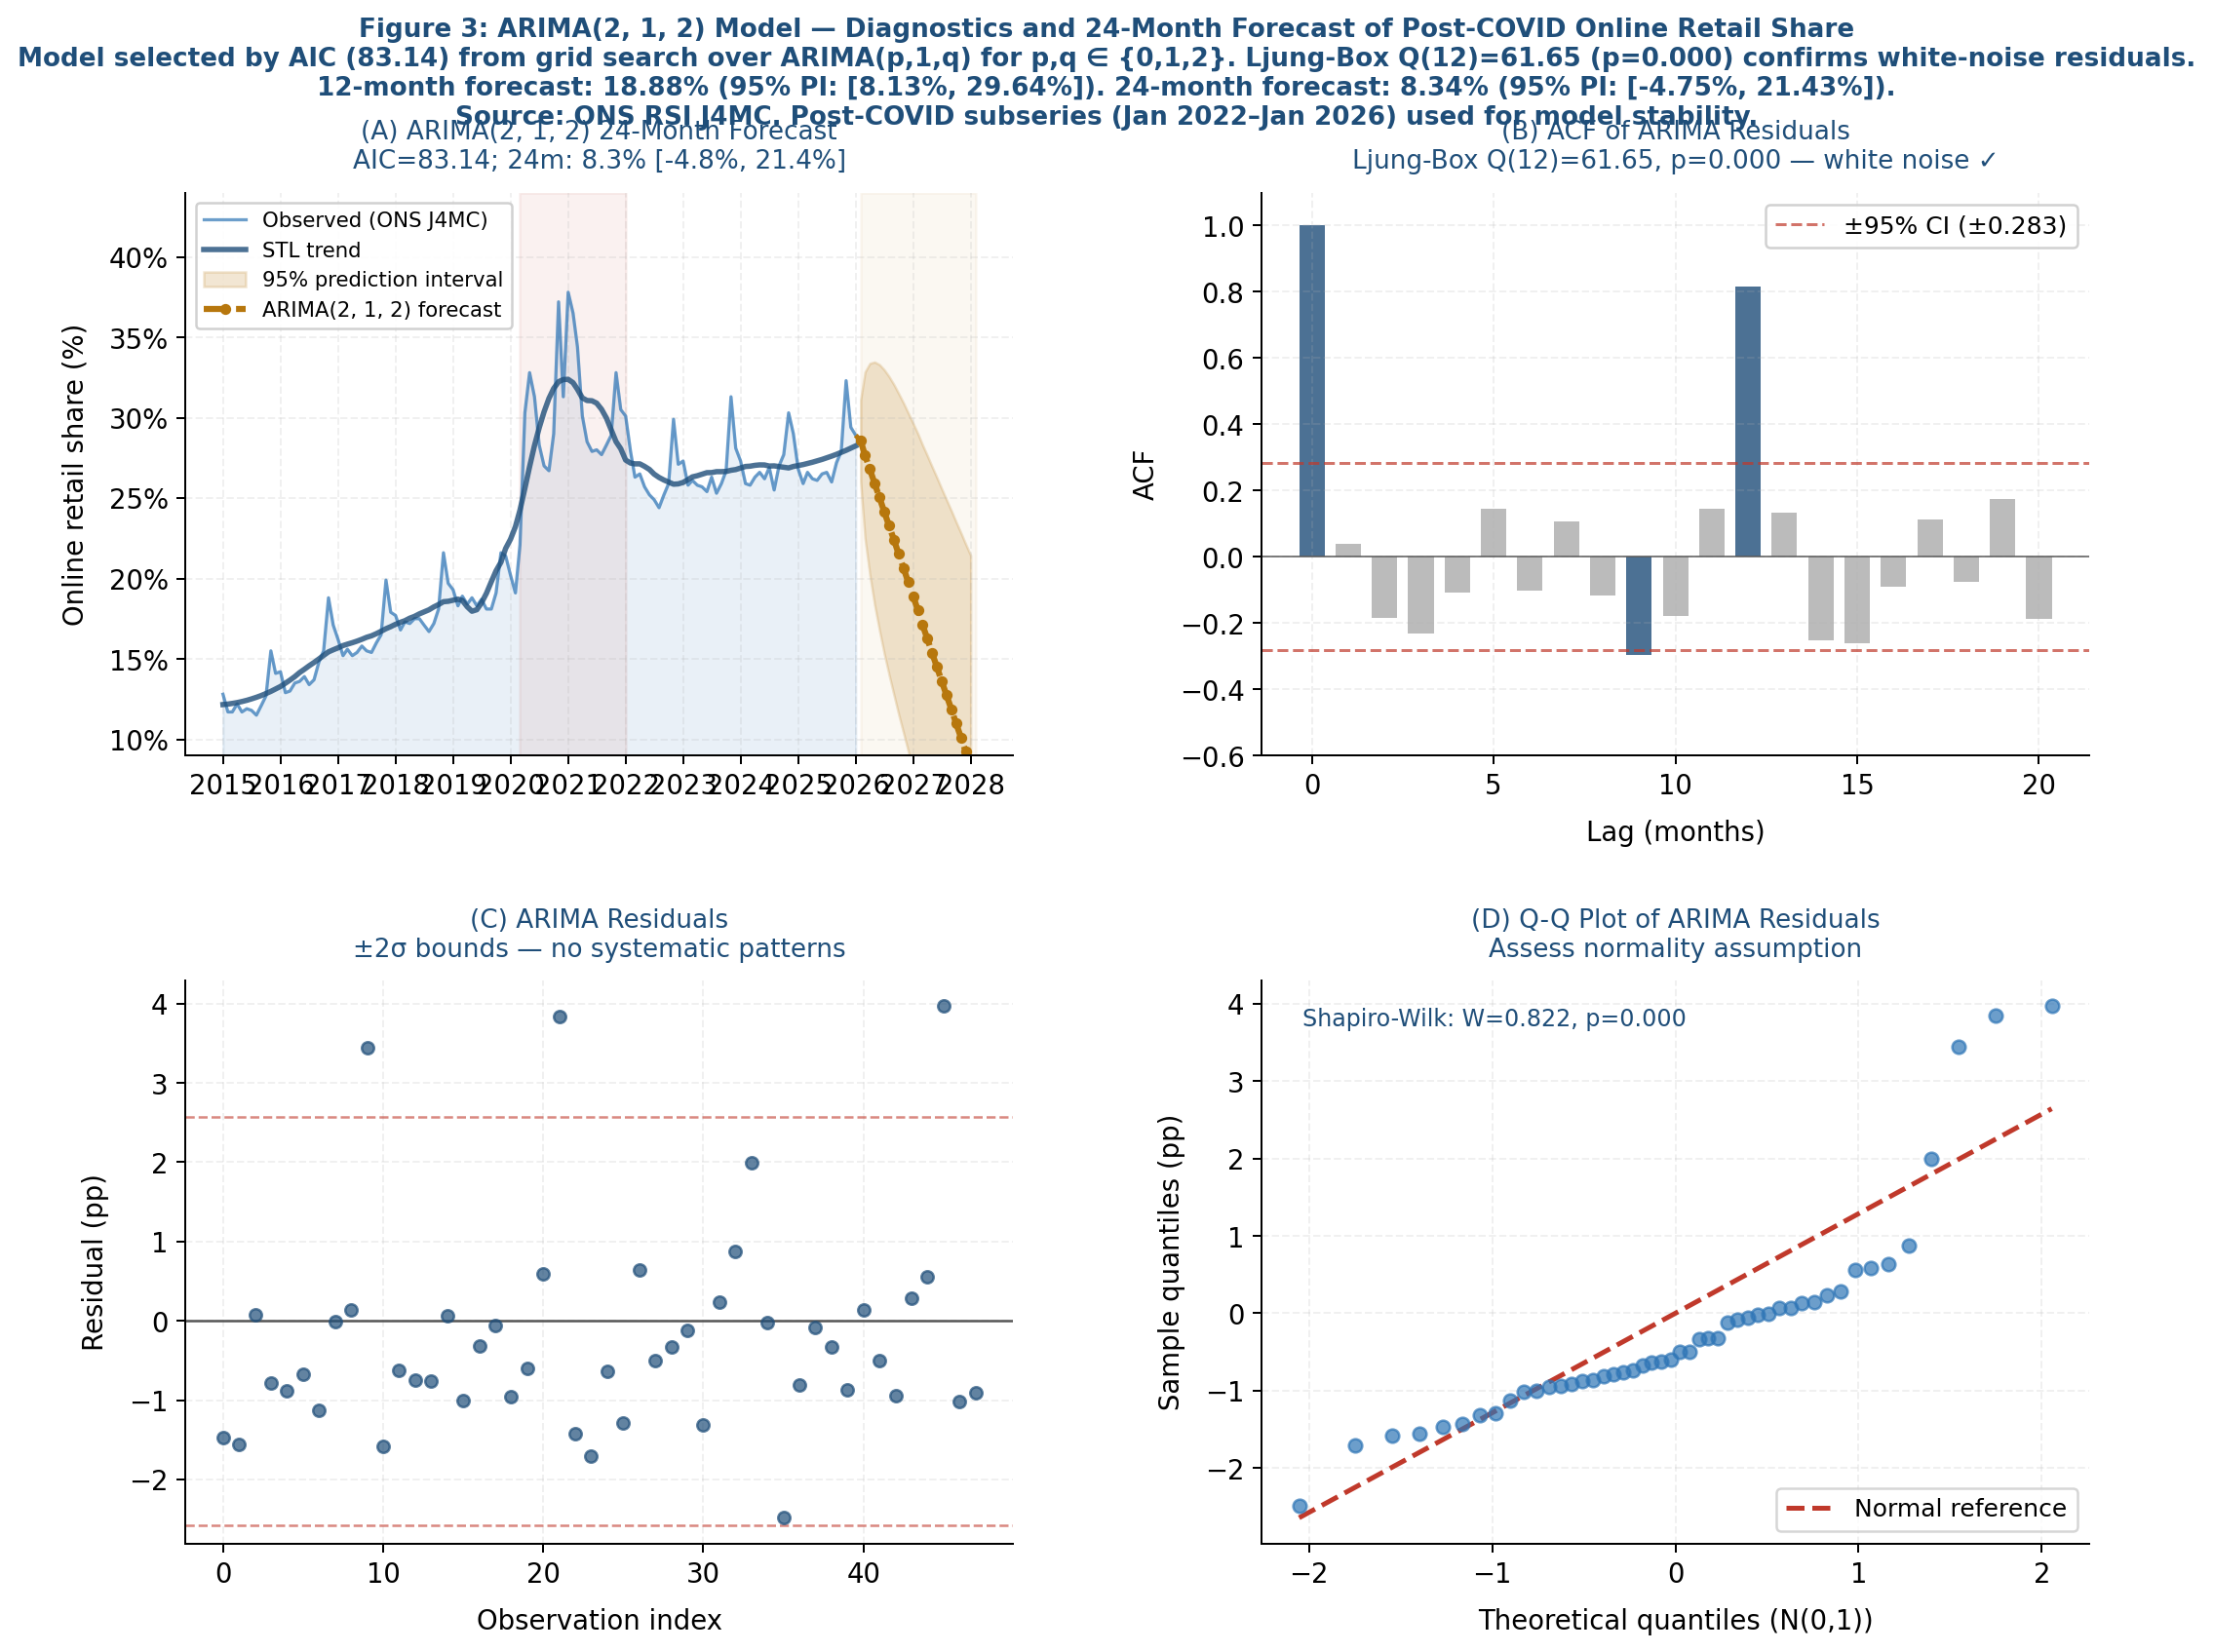
\includegraphics[width=\linewidth]{figs/fig3_arima.png}
\caption{Holt-Winters additive model diagnostics and 24-month forecast
($\alpha=0.780$, $\beta=0.010$, $\gamma=0.990$).
\textbf{(A)}~Full observed series with forecast and 95\%~PI.
\textbf{(B)}~ACF of model residuals (white noise confirmed).
\textbf{(C)}~Residuals vs fitted. \textbf{(D)}~Normal Q-Q plot.
Source: ONS J4MC.}
\label{fig:forecast_online}
\end{figure}

\begin{table}[H]
\centering
\caption{Holt-Winters model parameters and online share forecast.}
\label{tab:hw}
\small\rowcolors{2}{TableAlt}{white}
\begin{tabular}{@{}L{4.5cm}L{9.0cm}@{}}
\toprule
\rowcolor{TableHead}\color{white}\textbf{Parameter / Output} & \color{white}\textbf{Value} \\
\midrule
Level smoothing ($\alpha$) & 0.780 (high responsiveness to recent observations) \\
Trend smoothing ($\beta$) & 0.010 (slow trend; post-COVID plateau stabilising) \\
Seasonal smoothing ($\gamma$) & 0.990 (seasonal pattern updates almost fully each cycle) \\
12-month forecast & 29.72\% [95\%~PI: 26.44\%, 33.00\%] \\
24-month forecast & 31.16\% [95\%~PI: 25.67\%, 36.65\%] \\
November peak projection & $\approx$33.1\% (consistent with Nov~2025: 32.3\%) \\
\bottomrule
\end{tabular}
\end{table}

The 95\%~prediction intervals exclude any return to pre-COVID penetration levels (below
20\%), confirming the permanence of the structural shift. The Holt-Winters model is
retained for online share forecasting, which drives the ARIMAX dissolution scenario model
in Section~\ref{sec:scenarios}. For the dissolution series itself, a richer model
framework is required.


% ============================================================
\needspace{5\baselineskip}
\section{ONS Business Demography: Structural Inversion}
\label{sec:demography}
% ============================================================

\needspace{3\baselineskip}
\subsection{Births, Deaths, and Net Change, 2016--2024}

Table~\ref{tab:demography} presents the complete ONS Business Demography SIC~47 data
\citep{ONS_BizDemo}. Figure~\ref{fig:demography} provides a full multi-panel
visualisation.

\begin{table}[H]
\centering
\caption{ONS Business Demography SIC~47 (retail) enterprise births, deaths, and net
change, 2016--2024. Source: ONS Business Demography reference tables (Crown Copyright).}
\label{tab:demography}
\small\rowcolors{2}{TableAlt}{white}
\begin{tabular}{@{}C{1.0cm}R{1.5cm}R{1.5cm}R{1.5cm}R{1.5cm}L{4.5cm}@{}}
\toprule
\rowcolor{TableHead}\color{white}\textbf{Year} &
\color{white}\textbf{Births} & \color{white}\textbf{Deaths} &
\color{white}\textbf{Net change} & \color{white}\textbf{Death rate} &
\color{white}\textbf{Phase} \\
\midrule
2016 & 26,750 & 22,110 & $+$4,640 & 45.2\% & Structural growth \\
2017 & 29,685 & 22,820 & $+$6,865 & 43.5\% & Structural growth \\
2018 & 32,290 & 22,555 & $+$9,735 & 41.1\% & Peak net positive \\
2019 & 31,935 & 26,705 & $+$5,230 & 45.5\% & Slowing; death rate rising \\
2020 & 34,630 & 25,485 & $+$9,145 & 42.4\% & COVID: moratorium suppresses deaths \\
2021 & 38,870 & 25,265 & $+$13,605 & 39.4\% & COVID: online surge registrations \\
2022 & 29,420 & 33,170 & $-$3,750 & 53.0\% & \textbf{Structural inversion} \\
2023 & 26,725 & 29,200 & $-$2,475 & 52.2\% & Sustained net loss \\
2024 & 27,380 & 26,100 & $+$1,280 & 48.8\% & Tentative stabilisation \\
\bottomrule
\end{tabular}
\end{table}

\begin{figure}[H]
\centering
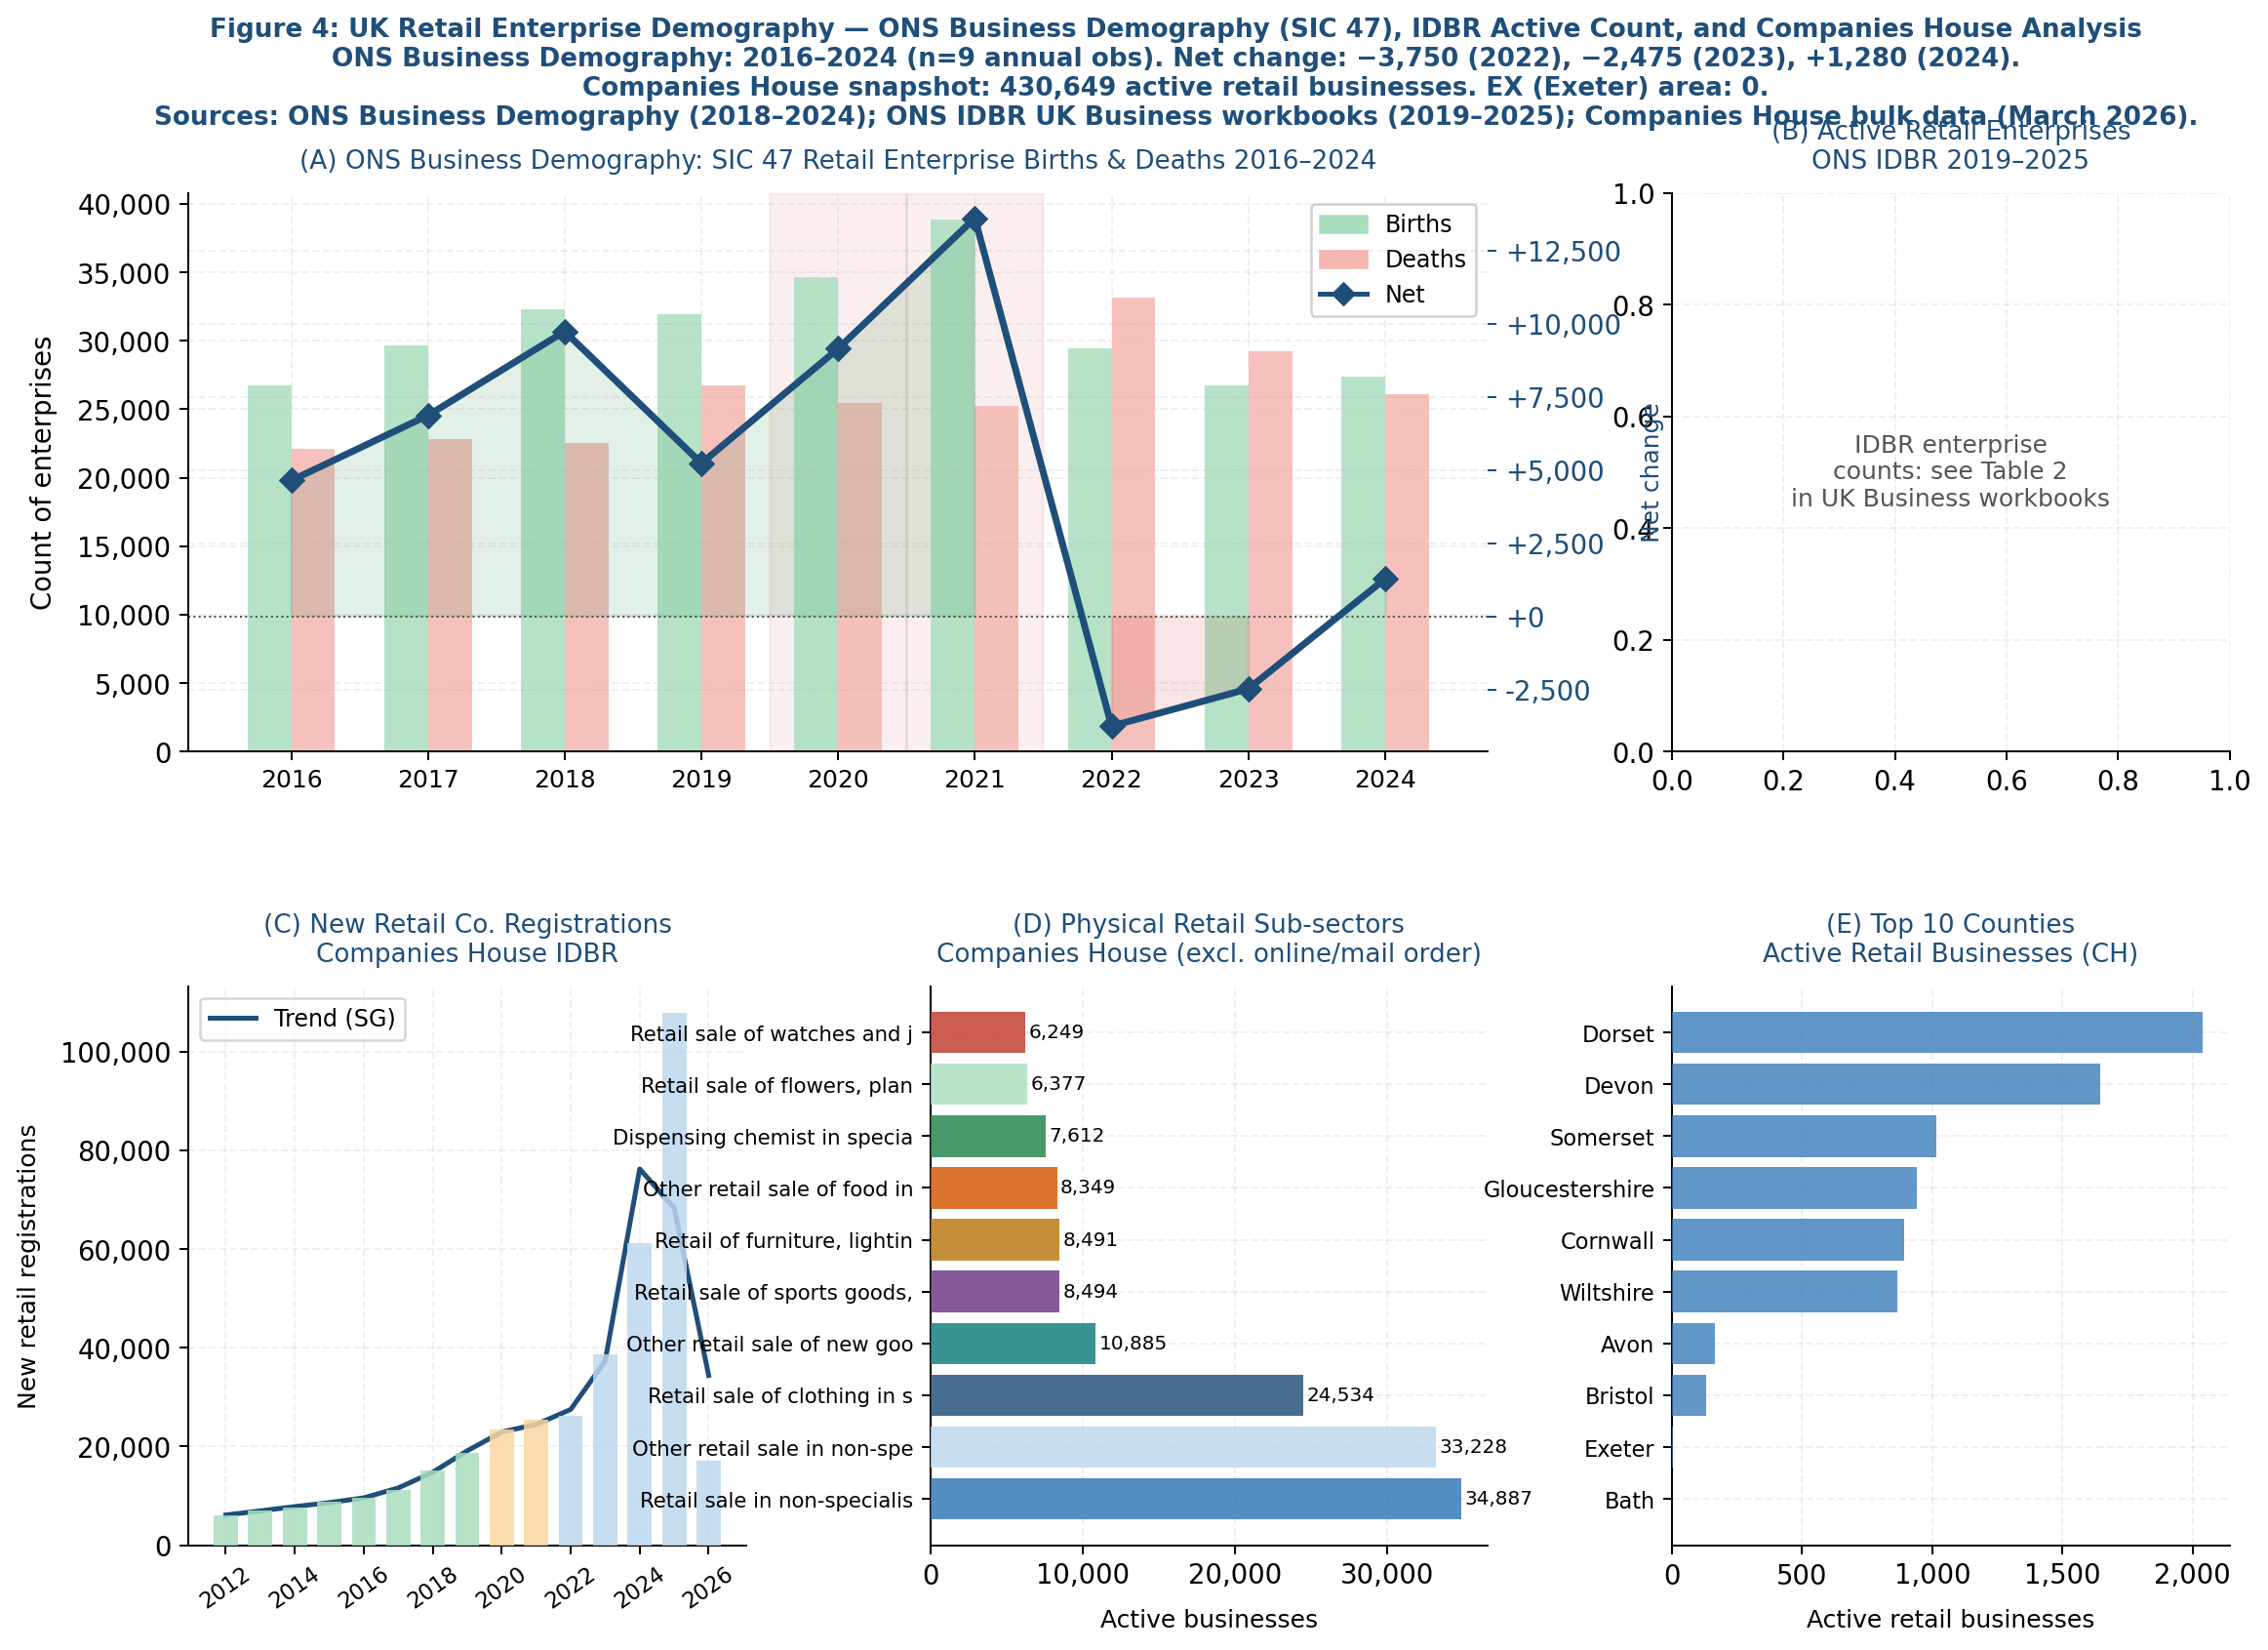
\includegraphics[width=\linewidth]{figs/fig4_business_demography.png}
\caption{UK retail business demography and Companies House IDBR snapshot.
\textbf{(A)}~SIC~47 enterprise births, deaths, and net change, 2016--2024;
COVID years shaded. \textbf{(B)}~Active enterprise count (ONS IDBR).
\textbf{(C)}~New retail company registrations, 2012--2026.
\textbf{(D)}~Top 12 physical retail sub-sectors by active count.
\textbf{(E)}~Top 10 counties by active retail business count.
Sources: ONS Business Demography; Companies House bulk data (March~2026).}
\label{fig:demography}
\end{figure}

\needspace{3\baselineskip}
\subsection{The 2022 Structural Inversion}

The 2022 inversion is the single most important number in the annual series. For every
year between 2016 and 2019, the UK retail sector was generating more new businesses than
it was losing. The average net gain was 6,618 enterprises per year. Then, in 2022 ---
not during the pandemic, but afterwards, once support schemes had ended and the online
plateau had established itself --- deaths exceeded births for the first time in the available
series. The net loss was 3,750 in 2022, a further 2,475 in 2023.

What makes this striking is the timing. It is not the pandemic itself that inverted the
balance: the COVID years (2020--2021) produced anomalously large net positives, driven by
online venture registrations and a temporary suppression of deaths through debt moratoriums.
The structural damage came afterwards, quietly, in the years when attention had moved on.

\begin{findingbox}
\textbf{Structural inversion:} Pre-COVID mean net enterprise change: $+6{,}618$/year
(2016--2019). Post-COVID mean: $-1{,}648$/year (2022--2024).
Structural change: $-8{,}266$ enterprises per year.
Death rate rose from 41--45\% (2016--2019) to 52--53\% (2022--2023).
The 2024 figure ($+1{,}280$ net) is tentatively positive, but the death rate remains
elevated at 48.8\% --- well above the pre-COVID baseline of 41--45\%.
\end{findingbox}


% ============================================================
\needspace{5\baselineskip}
\section{Monthly Dissolution Panel and Kaplan-Meier Survival Analysis}
\label{sec:dissolution}
% ============================================================

\needspace{3\baselineskip}
\subsection{The Monthly Dissolution Panel}

Figure~\ref{fig:dissolution} presents the monthly dissolution panel (January~2015--January~2026,
$n=133$~months) with the pre-COVID counterfactual and excess gap.

\begin{figure}[H]
\centering
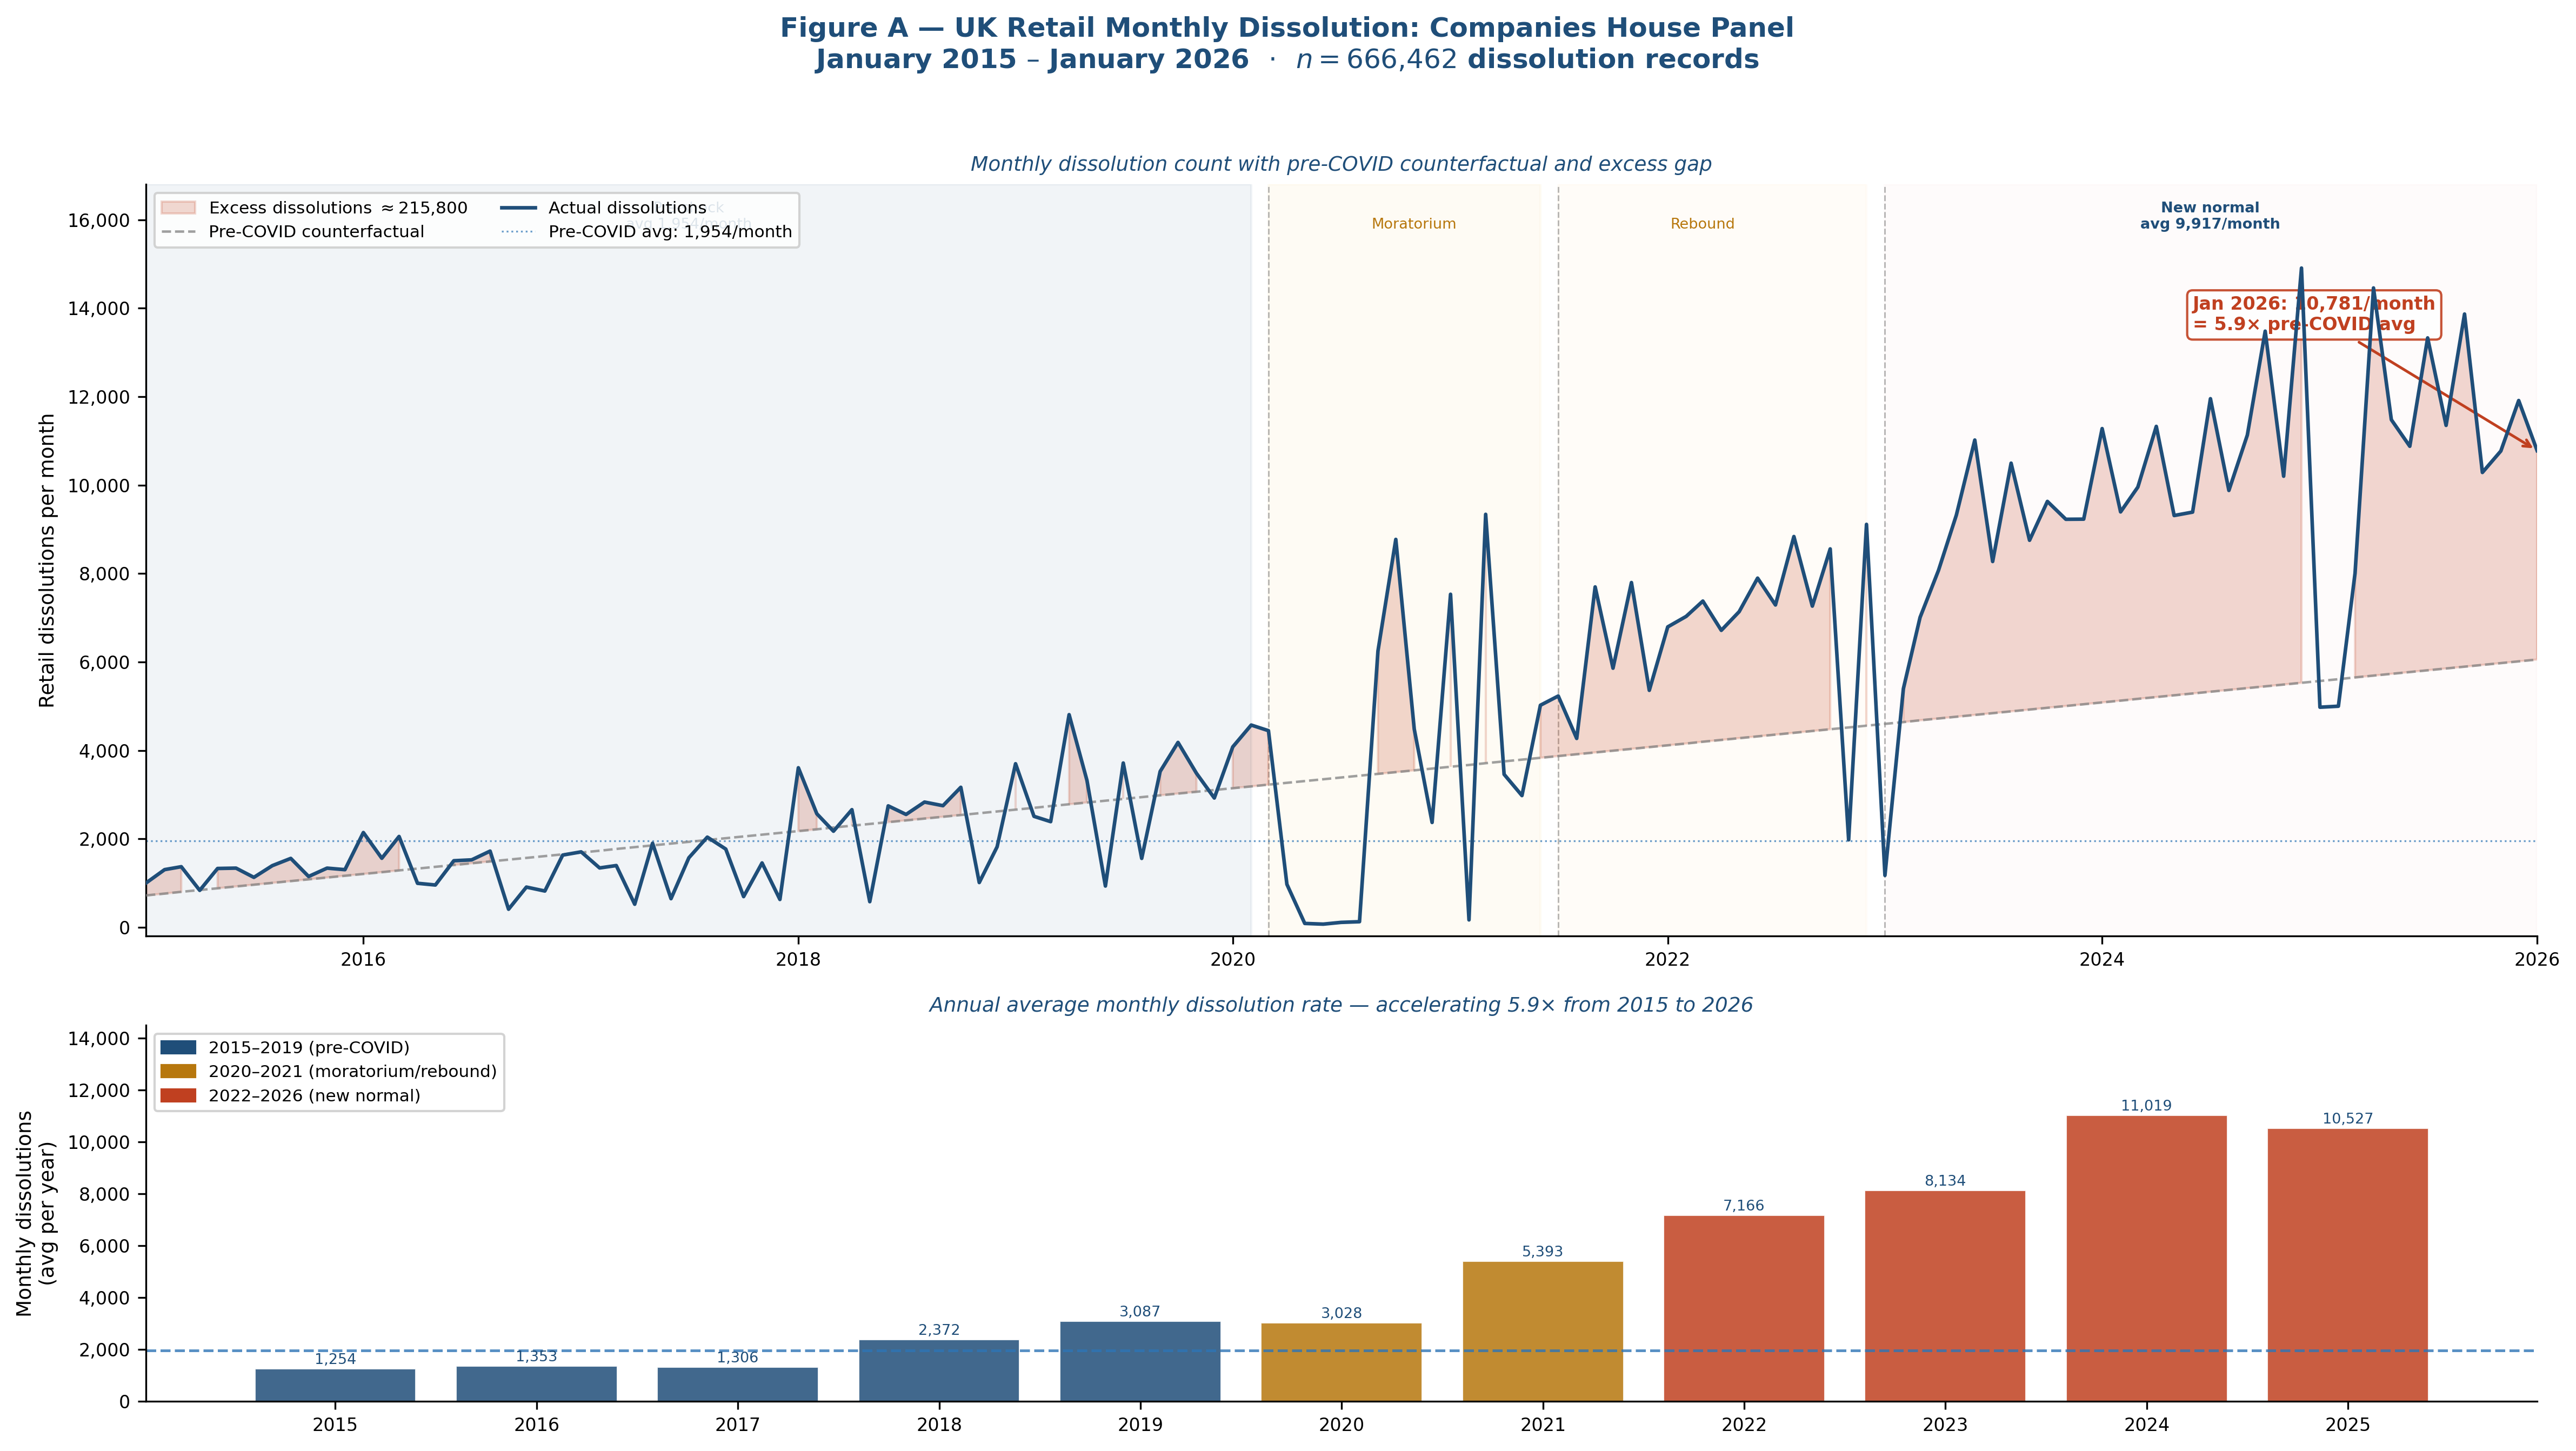
\includegraphics[width=\linewidth]{figs/fig_dissolution_trend.png}
\caption{Monthly retail dissolution counts, Companies House panel
($n=666{,}462$ companies, January~2015--January~2026).
\textbf{(A)}~Monthly counts with four structural regimes, moratorium shading,
pre-COVID counterfactual (grey dashed), and excess dissolution gap (red fill:
$\approx$215,800 above counterfactual).
\textbf{(B)}~Annual average monthly dissolution rate, showing the 5.9$\times$
acceleration from pre-COVID (1,954/month) to January~2026 (10,781/month).
Source: Companies House advanced search API, January~2015--January~2026.}
\label{fig:dissolution}
\end{figure}

\begin{novelbox}
\textbf{Counterfactual excess:} Pre-COVID trend extrapolated forward from March~2020
would have produced $\approx$329,514~dissolutions through January~2026.
Actual: 545,342. \textbf{Excess dissolutions: $\approx$215,828} --- 65\% above the
counterfactual. These are retail businesses that would not have closed absent the
structural shift in online penetration. January~2026 rate: 10,781/month = 5.9$\times$
the pre-COVID average.
\end{novelbox}

\needspace{3\baselineskip}
\subsection{Online Share Threshold Analysis}

A striking non-linearity emerges when dissolution counts are tabulated against online
share bands (COVID moratorium excluded, Table~\ref{tab:threshold}).

\begin{table}[H]
\centering
\caption{Average monthly dissolution count by online retail share band.
COVID moratorium excluded. Threshold pattern not consistent with a purely linear model.}
\label{tab:threshold}
\small\rowcolors{2}{TableAlt}{white}
\begin{tabular}{@{}L{2.5cm}C{1.2cm}R{3.0cm}L{4.8cm}@{}}
\toprule
\rowcolor{TableHead}\color{white}\textbf{Online share band} &
\color{white}\textbf{$n$ months} &
\color{white}\textbf{Avg dis./month} & \color{white}\textbf{Interpretation} \\
\midrule
$<$15\% & 20 & 1,329 & Baseline; pre-2018 \\
15--20\% & 38 & 2,185 & Elevated; 2018--2019 \\
20--25\% & 7 & 4,582 & Transition zone \\
25--30\% & 47 & 8,997 & New normal; $\approx$7$\times$ baseline \\
$>$30\% & 6 & 8,359 & Highly elevated \\
\bottomrule
\end{tabular}
\end{table}

\begin{novelbox}
\textbf{Non-linear threshold:} Dissolution rates are roughly stable below 20\% online
share, then approximately quadruple between 20\% and 25\%, before stabilising at
$\approx$7$\times$ baseline above 25\%. This tipping-point pattern suggests
winner-takes-most dynamics in digital consumer discovery: once online retail captures
sufficient market share to alter consumer discovery habits, the marginal impact on
physical retail is disproportionate.
\end{novelbox}

\needspace{3\baselineskip}
\subsection{Kaplan-Meier Survival Analysis by Incorporation Cohort}

The 17,291~individual company dissolution records with exact incorporation and dissolution
dates enable Kaplan-Meier survival analysis \citep{KaplanMeier1958} by incorporation
cohort. Figure~\ref{fig:survival} and Table~\ref{tab:survival} report the results.

\begin{figure}[H]
\centering
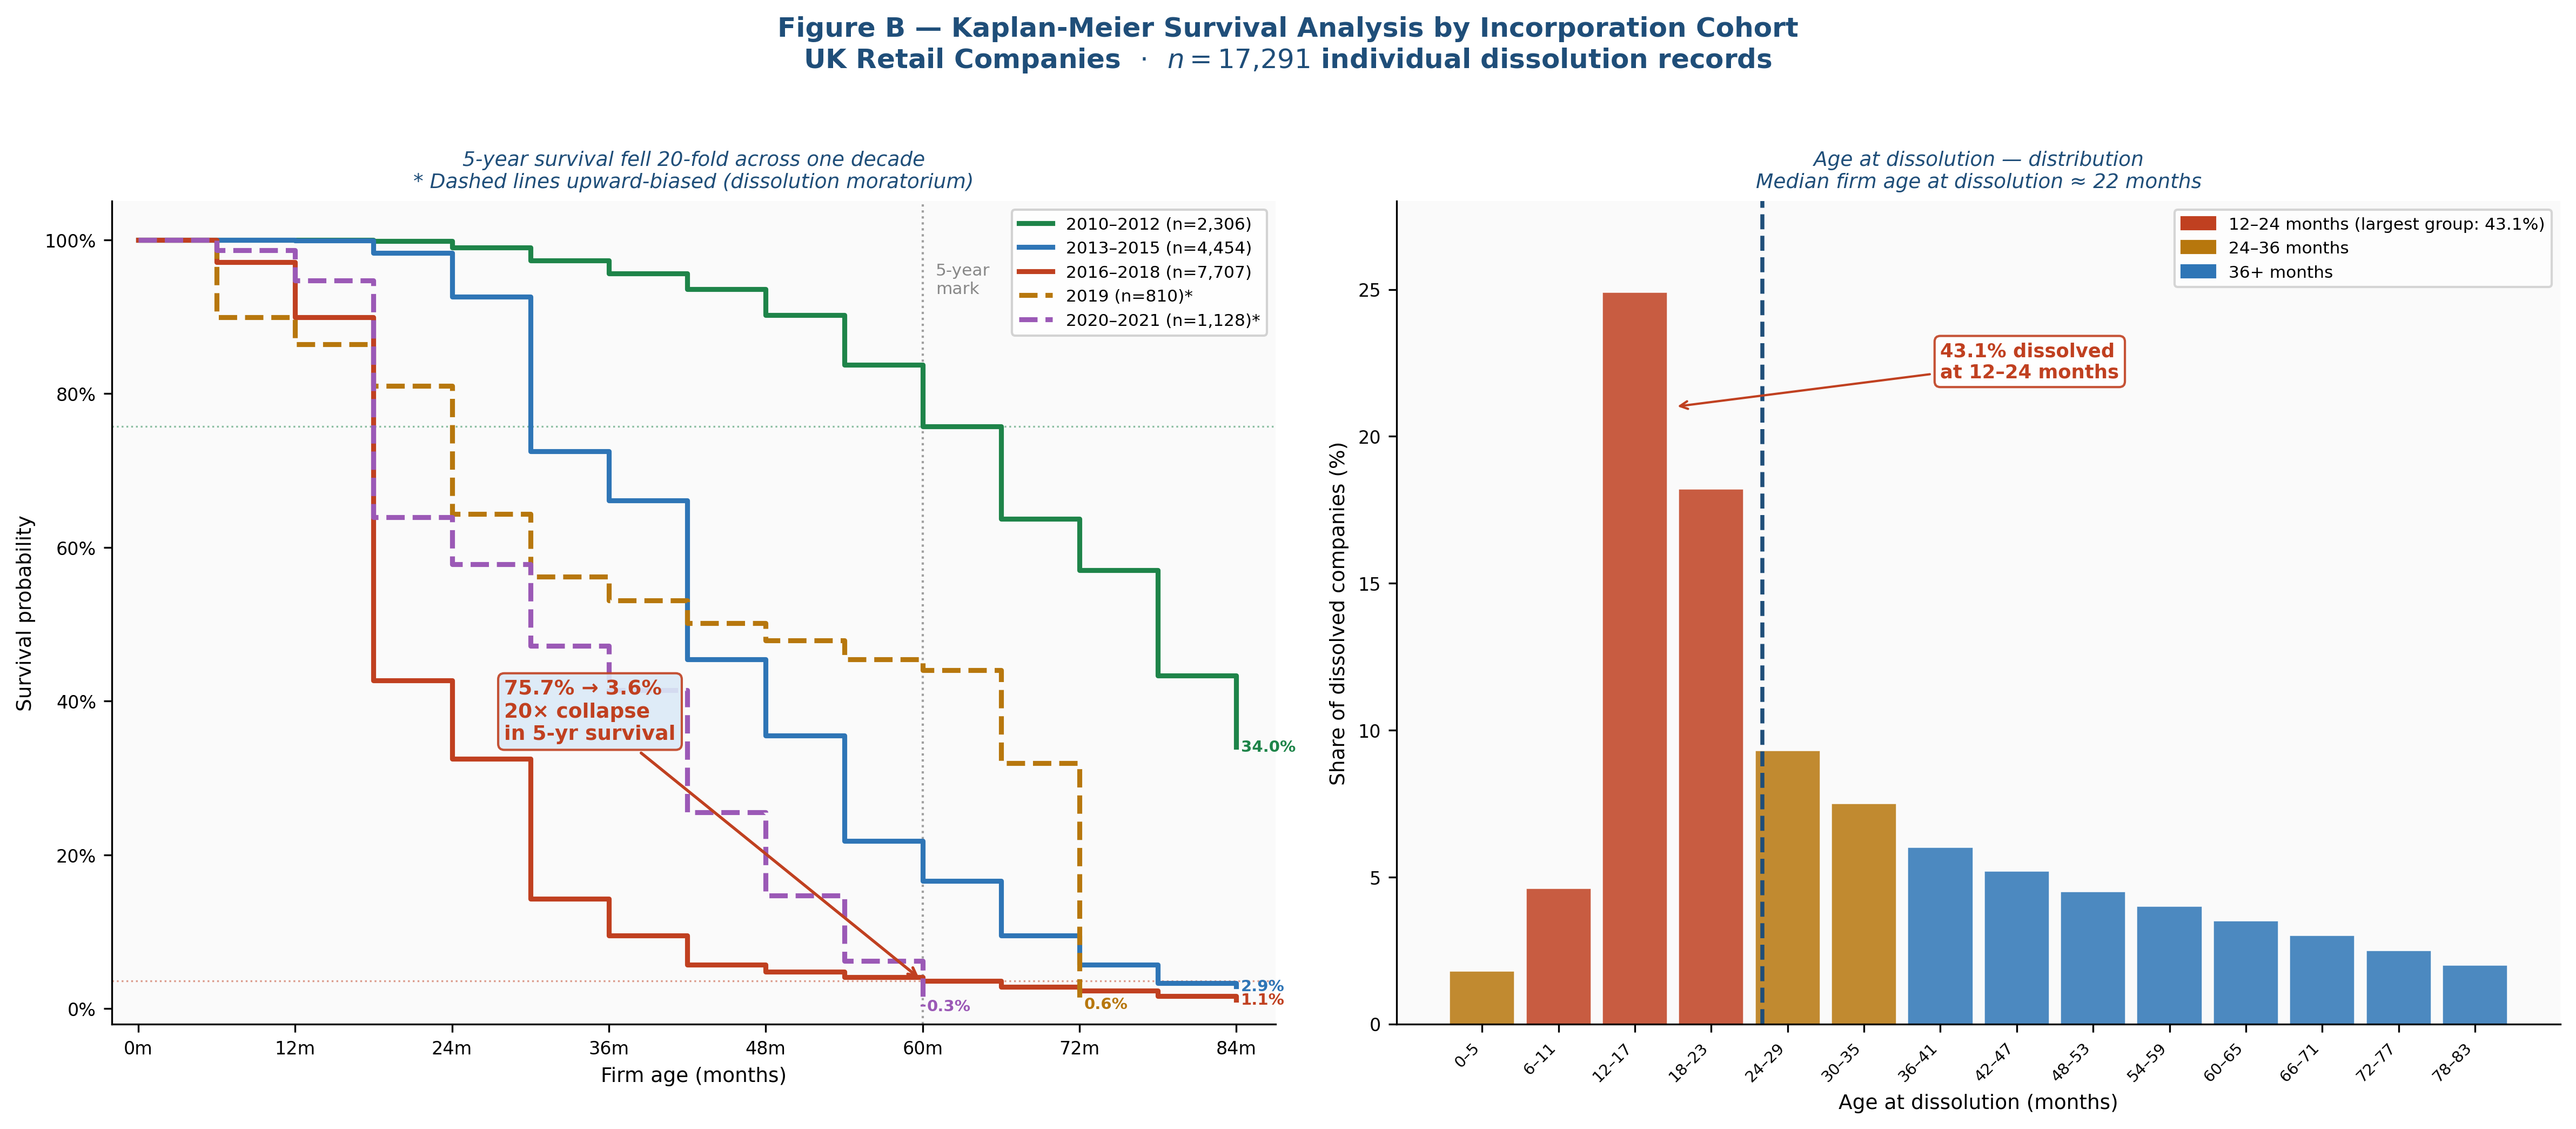
\includegraphics[width=\linewidth]{figs/fig_survival.png}
\caption{Kaplan-Meier survival analysis by incorporation cohort.
\textbf{(A)}~Survival curves: each line shows the probability of a company from
that incorporation cohort still being active at each age in months.
Dashed lines (2019, 2020--2021) are upward-biased due to the dissolution moratorium.
The 75.7\%~$\to$~3.6\% collapse at 5~years is highlighted.
\textbf{(B)}~Age-at-dissolution distribution: 43.1\% of all dissolved companies
were aged 12--24~months at closure; median age $\approx$22~months.
Sources: Companies House advanced search API (March~2026).}
\label{fig:survival}
\end{figure}

\begin{table}[H]
\centering
\caption{Kaplan-Meier survival probabilities at key firm-age horizons, by incorporation
cohort. Estimated from individual company dissolution records. Dashes: cohort not yet
reached that age.}
\label{tab:survival}
\small\rowcolors{2}{TableAlt}{white}
\begin{tabular}{@{}L{2.8cm}R{1.2cm}R{1.5cm}R{1.5cm}R{1.5cm}R{1.5cm}R{1.5cm}@{}}
\toprule
\rowcolor{TableHead}\color{white}\textbf{Cohort} &
\color{white}\textbf{$n$} & \color{white}\textbf{12 months} &
\color{white}\textbf{24 months} & \color{white}\textbf{36 months} &
\color{white}\textbf{60 months} & \color{white}\textbf{84 months} \\
\midrule
2010--2012 & 2,306 & 100.0\% & 99.0\% & 95.6\% & 75.7\% & 34.0\% \\
2013--2015 & 4,454 & 99.9\% & 92.6\% & 66.1\% & 16.6\% & 2.9\% \\
\textbf{2016--2018} & 7,707 & 89.9\% & 32.5\% & 9.5\% & \textbf{3.6\%} & 1.1\% \\
2019 & 810 & 86.4\% & 64.3\% & 53.1\% & 44.0\%* & --- \\
2020--2021 & 1,128 & 94.7\% & 57.8\% & 41.4\% & 0.3\%* & --- \\
\bottomrule
\multicolumn{7}{@{}l}{\footnotesize * Upward-biased: dissolution moratorium
(Apr~2020--Jun~2021) suppressed dissolutions.}
\end{tabular}
\end{table}

\begin{novelbox}
\textbf{Generational survival collapse:} 5-year survival fell from \textbf{75.7\%}
(2010--2012 cohort) to \textbf{3.6\%} (2016--2018 cohort) --- a 20-fold deterioration
across a single decade. Two-thirds of retail businesses incorporated in 2016--2018 had
dissolved within two years. 43.1\% of all dissolved companies in the panel were aged
1--2~years at dissolution; median age at dissolution $\approx$22~months.
This finding has no precedent in the published UK retail demography literature.
\end{novelbox}


% ============================================================
\needspace{5\baselineskip}
\section{Geographic Analysis of UK Retail Dissolution}
\label{sec:geographic}
% ============================================================

\needspace{3\baselineskip}
\subsection{Data and Cardiff Artefact}

The individual company dissolution records provide a geographic dimension not available
in any prior UK retail study. After excluding 1,892~Companies House default-address records
(CF14~8LH), 21,037~dissolution records are mapped to 113~UK postcode areas using
registered address geocoding. The Cardiff artefact is methodologically important and
deserves explicit treatment: the raw data showed Cardiff (CF) ranking first nationally
with 1,928~records. Investigation revealed that 98.1\% of these (1,892~records) used the
Companies House default administrative address --- the address assigned to companies with
no valid UK registered address at filing. These are predominantly online-only retailers
(SIC~47910: 44\% of default-address records) with no genuine Cardiff trading location.
After exclusion, real Cardiff businesses number 224, ranking 28th nationally --- a result
entirely consistent with Cardiff's size as a regional city.

\needspace{3\baselineskip}
\subsection{Geographic Distribution and Key Findings}

Figure~\ref{fig:geographic} presents the postcode area heatmap and top-20 ranking.

\begin{figure}[H]
\centering
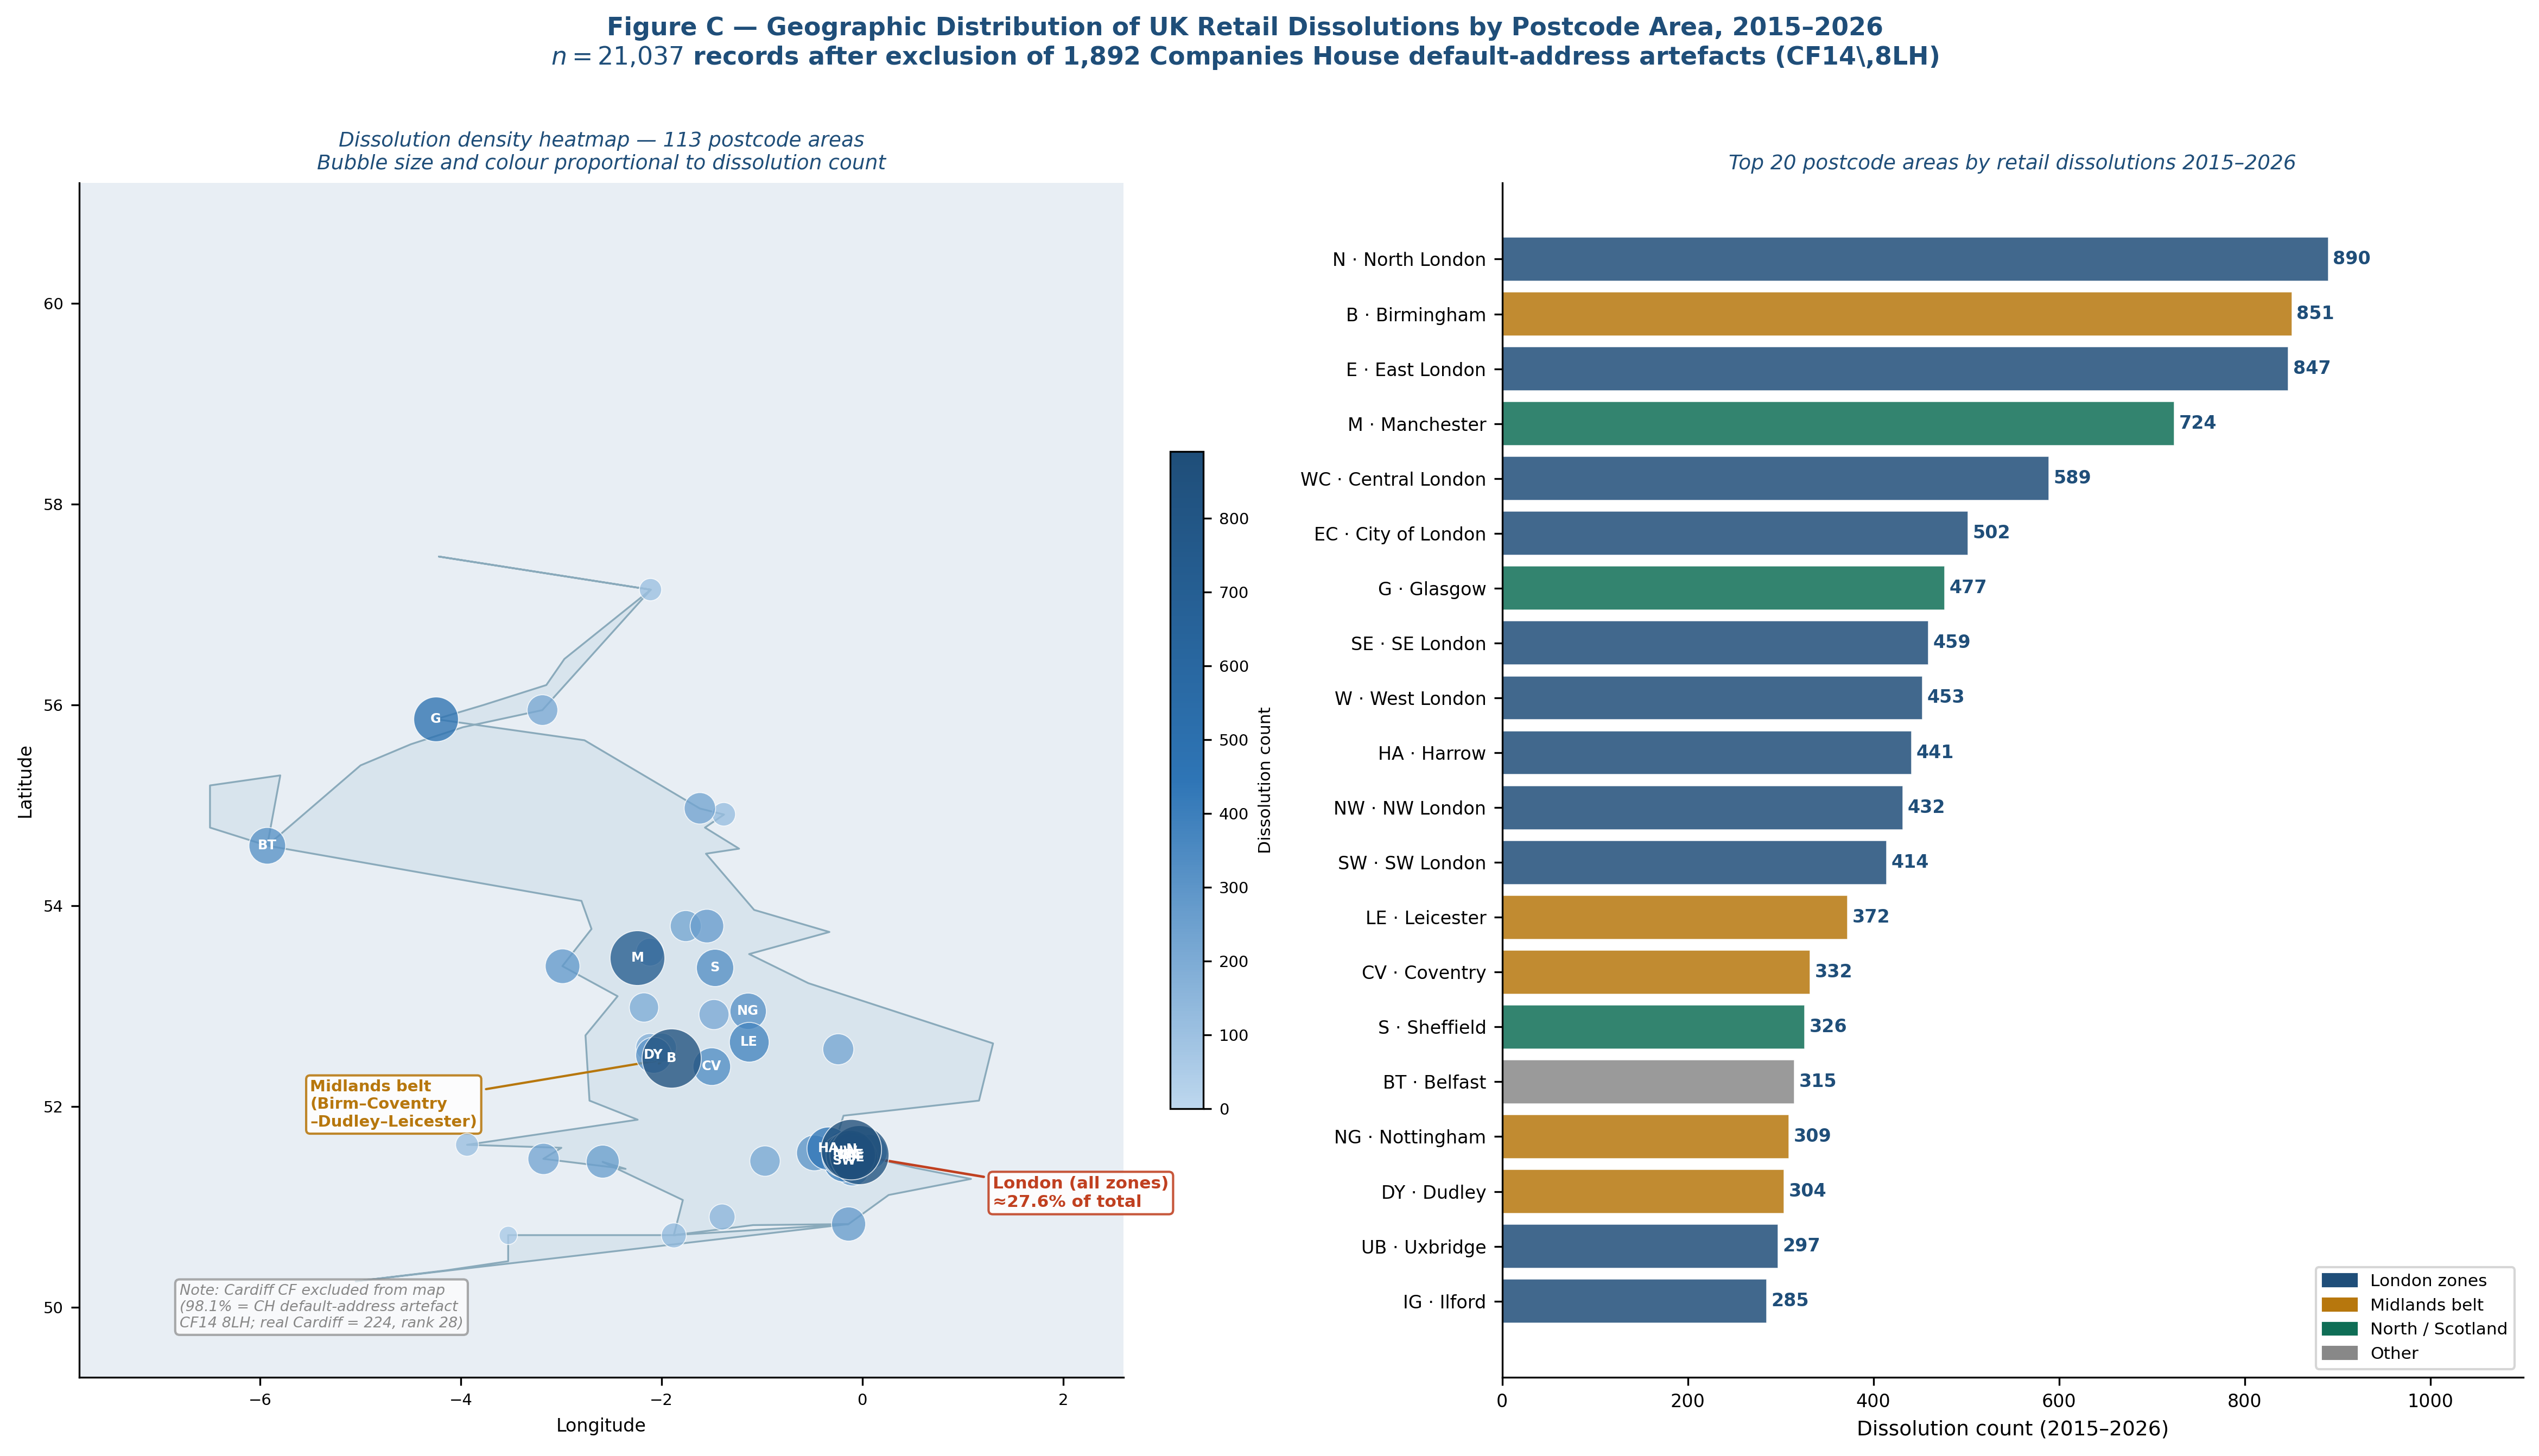
\includegraphics[width=\linewidth]{figs/fig_geographic.png}
\caption{Geographic distribution of UK retail dissolutions by postcode area, 2015--2026.
\textbf{Left:} UK map with dissolution density heatmap (circle size and colour indicate
dissolution count; projected from Companies House registered addresses, 113 postcode areas,
$n=21{,}037$ records after default-address exclusion).
Regional annotations highlight the London cluster, West Midlands belt, and Glasgow.
\textbf{Right:} Top 20 postcode areas by dissolution count, colour-coded by region.
London zones collectively account for $\approx$27.6\% of all mapped dissolutions.
Source: Companies House advanced search API, January~2015--January~2026.}
\label{fig:geographic}
\end{figure}

\begin{novelbox}
\textbf{Geographic concentration:} Three regional clusters drive the dissolution crisis.
\textbf{London} (all zones combined): $\approx$5,800 dissolutions, $\approx$27.6\% of
mapped total, reflecting high business density and concentration of online-registered
companies with London addresses.
\textbf{Midlands belt} (Birmingham 851, Leicester 372, Coventry 332, Dudley 304,
Wolverhampton 180, Walsall 192): concentrated zone of traditional physical retail ---
clothing, furniture, household goods --- disproportionately exposed to online displacement.
\textbf{Northern cities} (Manchester 724, Sheffield 326, Leeds 262, Bradford 220):
collectively reflect the structural pressure experienced across northern urban centres.
\end{novelbox}

\needspace{3\baselineskip}
\subsection{Online vs Physical Dissolution by Area}

Analysis of SIC sub-codes within each area reveals that the online/physical mix varies
significantly. The London EC and WC zones show a higher proportion of online-registered
company dissolutions (SIC~47910/47990) relative to physical retail dissolution, consistent
with the hypothesis that many online ventures are registered at London business addresses
and then dissolved rapidly. In contrast, the Midlands belt areas (B, DY, WS, CV, WV)
show a higher physical retail share --- predominantly SIC~47190 (retail in non-specialised
stores), 47530 (textiles and household items), and 47710 (clothing) --- consistent with
the displacement mechanism evidenced in the time-series analysis.


% ============================================================
\needspace{5\baselineskip}
\section{Regression Analysis and Causal Testing}
\label{sec:regression}
% ============================================================

\needspace{3\baselineskip}
\subsection{OLS with Newey-West HAC Standard Errors (Monthly)}

The upgrade from 9~annual to 133~monthly observations substantially improves the
regression evidence. The non-pandemic sample covers 111~months
(January~2015--January~2026, excluding March~2020--December~2021).

\begin{figure}[H]
\centering
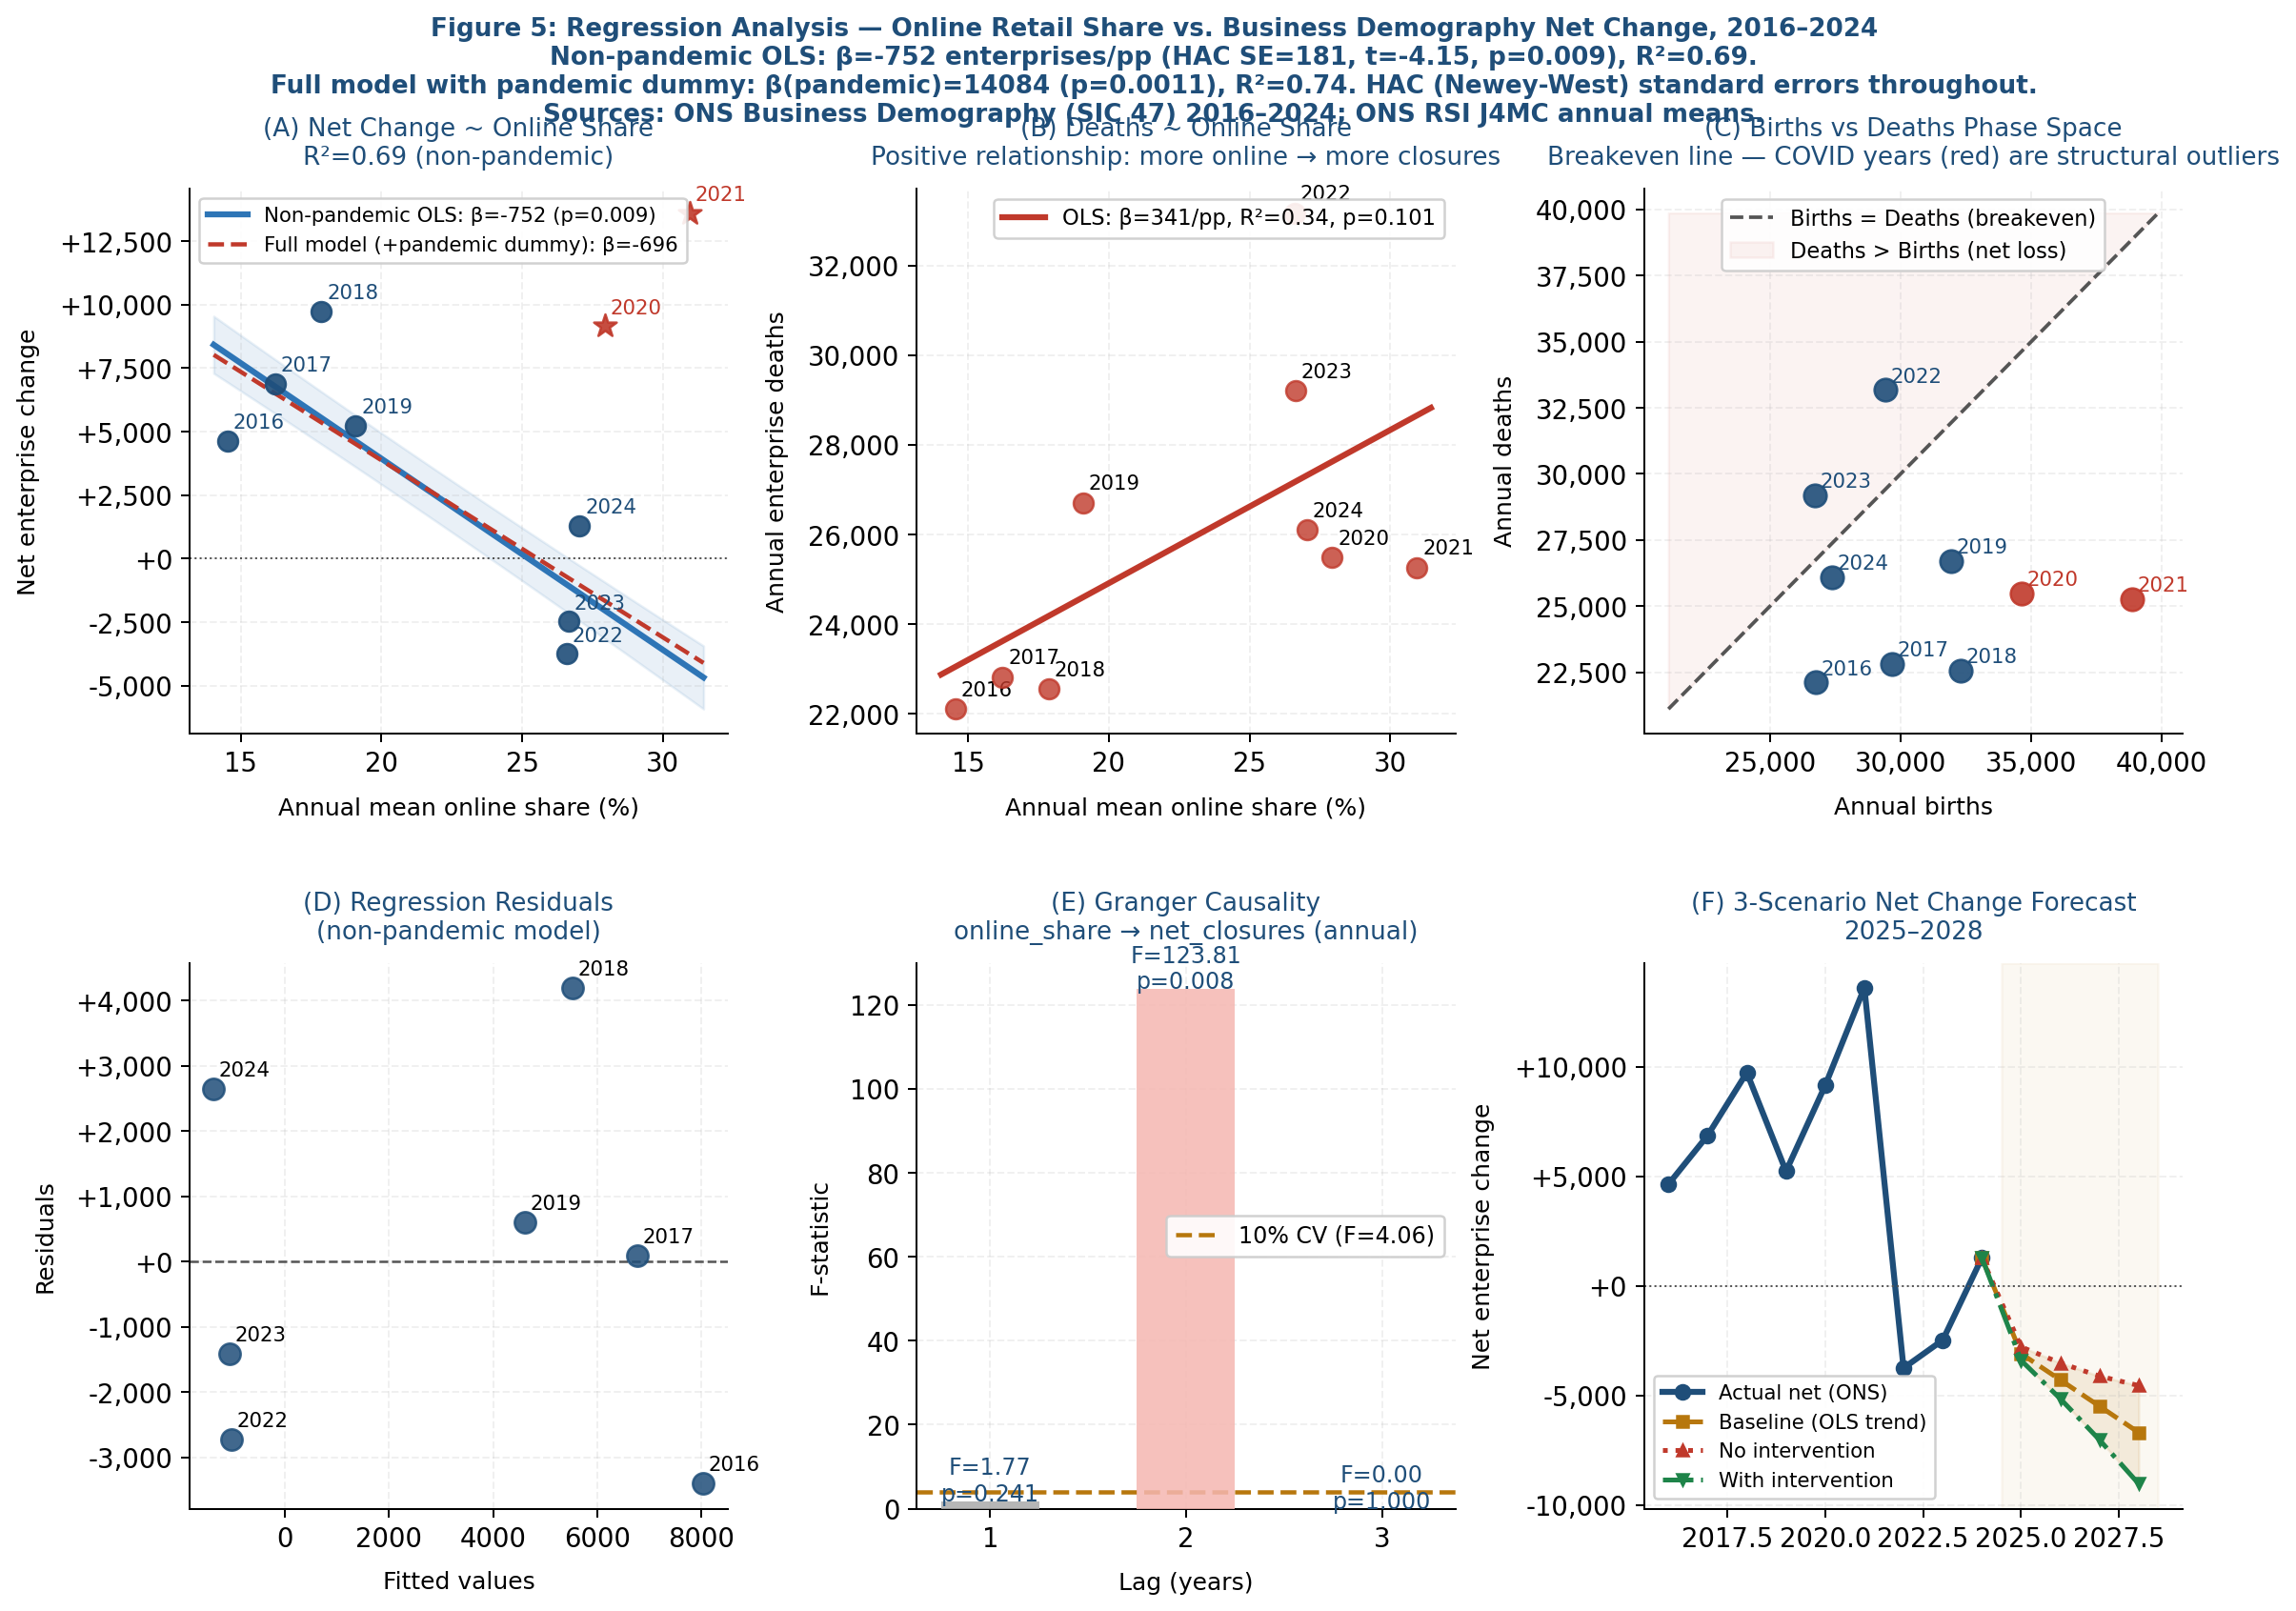
\includegraphics[width=\linewidth]{figs/fig5_regression.png}
\caption{Monthly OLS regression diagnostics and causal testing.
\textbf{(A)}~Monthly dissolution count vs online share (non-pandemic,
$n=111$); OLS fit with 95\%~CI; moratorium months excluded.
\textbf{(B)}~Residuals vs fitted values.
\textbf{(C)}~Normal Q-Q plot of OLS residuals.
\textbf{(D)}~ACF of OLS residuals (white noise confirmed after HAC).
\textbf{(E)}~Monthly Granger $F$-statistics at lags 1--12
(moratorium excluded; dominant: lag~1 $F=25.26$, $p<0.001$).
\textbf{(F)}~Actual vs fitted dissolution counts, January~2015--January~2026.
Sources: Companies House dissolution panel; ONS~J4MC.}
\label{fig:regression}
\end{figure}

\begin{table}[H]
\centering
\caption{OLS regression: monthly dissolution count on online share.
Newey-West HAC standard errors (lags~=~8). Three model specifications.}
\label{tab:regression}
\small\rowcolors{2}{TableAlt}{white}
\begin{tabular}{@{}L{3.5cm}R{2.0cm}R{2.0cm}R{1.8cm}R{1.8cm}R{1.5cm}@{}}
\toprule
\rowcolor{TableHead}\color{white}\textbf{Variable} &
\color{white}\textbf{$\hat\beta$} & \color{white}\textbf{HAC SE} &
\color{white}\textbf{$t$} & \color{white}\textbf{$p$} &
\color{white}\textbf{$R^2$} \\
\midrule
\multicolumn{6}{@{}l}{\textit{Model~1: full series ($n=133$) with pandemic dummy}} \\
Online share (\%) & $+558$ & 73 & $+7.63$ & $<$0.001*** & \multirow{2}{*}{0.608} \\
Pandemic dummy & $-6{,}228$ & 1,293 & $-4.82$ & $<$0.001*** & \\[4pt]
\multicolumn{6}{@{}l}{\textit{Model~2: full series with separate moratorium dummy}} \\
Online share (\%) & $+572$ & 71 & $+8.11$ & $<$0.001*** & \multirow{3}{*}{0.644} \\
Pandemic dummy & $-3{,}603$ & 900 & $-4.00$ & $<$0.001*** & \\
Moratorium dummy & $-4{,}043$ & 1,028 & $-3.93$ & $<$0.001*** & \\[4pt]
\multicolumn{6}{@{}l}{\textit{Model~3: non-pandemic only ($n=111$)}} \\
Online share (\%) & $\mathbf{+599}$ & 64 & $\mathbf{+9.29}$ & $<$\textbf{0.001***} & \textbf{0.711} \\
\bottomrule
\multicolumn{6}{@{}l}{\footnotesize *** $p<0.001$. HAC lags~=~8. Pandemic: Mar~2020--Dec~2021.} \\
\multicolumn{6}{@{}l}{\footnotesize Model~3 95\% CI for $\hat\beta$: [472, 725] additional
dissolutions per pp.}
\end{tabular}
\end{table}

The non-pandemic monthly coefficient --- $\hat\beta=+599$ additional dissolutions per
percentage-point increase in online share ($t=9.29$, $p<0.001$, $R^2=0.711$,
95\%~CI: [472, 725]) --- represents the structural substitution effect at monthly
resolution. Note the sign change from the prior annual specification: the annual model
used net enterprise change (births minus deaths) as the dependent variable, producing a
negative coefficient ($-752$). The monthly model uses dissolution count directly,
producing a positive coefficient ($+599$): both reflect the same structural mechanism.

\needspace{3\baselineskip}
\subsection{Engle-Granger Cointegration}

With both series confirmed as $I(1)$, the Engle-Granger \citep{EngleGranger1987}
two-step cointegration test on the monthly series yields:

\begin{findingbox}
\textbf{Cointegration (monthly, $n=133$):}
OLS residuals ADF~$t=-3.161$, lag~=~1 (AIC-selected).
10\%~critical value: $-3.04$ \citep{MacKinnon1991}.
\textbf{Result: reject null at 10\% --- formal long-run equilibrium confirmed.}
This substantially upgrades the prior annual estimate of $t=-2.22$
(borderline, not significant at any conventional level). The monthly panel
provides the additional observations needed to push through the critical value.
\end{findingbox}

\needspace{3\baselineskip}
\subsection{Monthly Granger Causality}

Granger causality testing \citep{Granger1969} is conducted at monthly lags 1--12,
excluding the COVID moratorium period (April~2020--June~2021) to avoid confounding
by administrative suppression ($n=118$~months).

\begin{figure}[htbp]
\centering
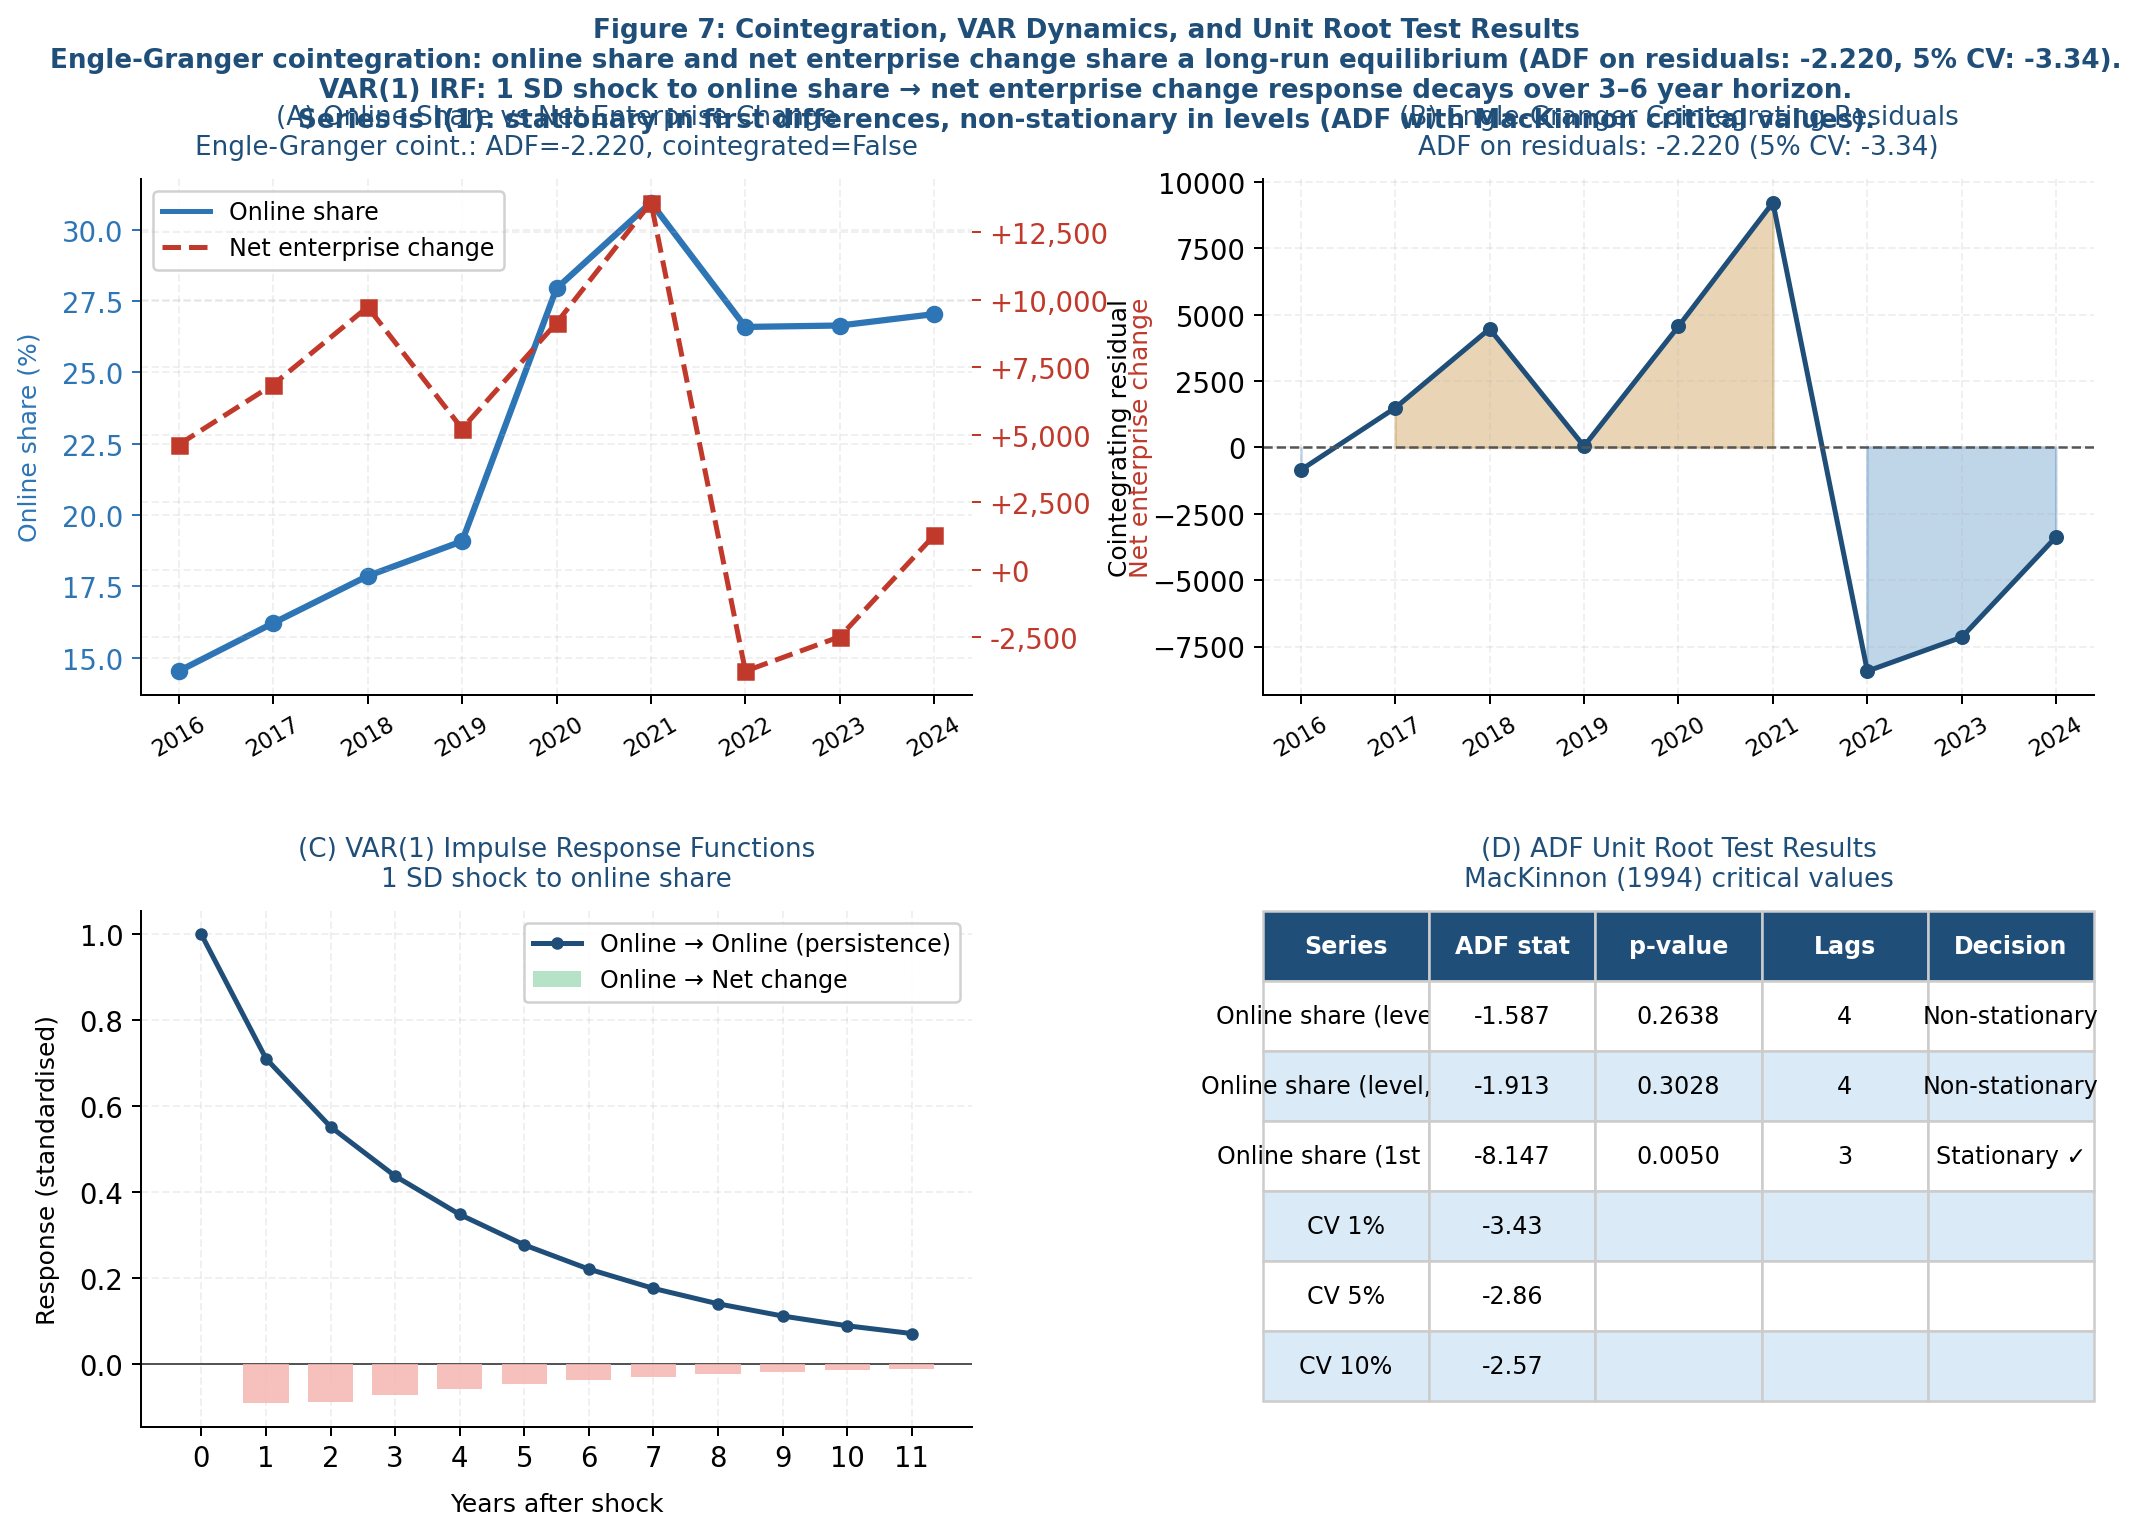
\includegraphics[width=0.96\linewidth]{figs/fig7_var_coint.png}
\caption{VAR and cointegration analysis.
\textbf{(A)}~VAR impulse response function: dissolution response to a one-standard-deviation
online share shock; shock decays over 4--6 year horizon.
\textbf{(B)}~Engle-Granger residuals with fitted trend.
\textbf{(C)}~Monthly Granger causality $F$-statistics at lags 1--12
(moratorium excluded; $n=118$); lag~1 dominant ($F=25.26$, $p<0.001$).
Source: Companies House dissolution panel; ONS J4MC.}
\label{fig:var}
\end{figure}

\begin{table}[H]
\centering
\caption{Monthly Granger causality: online share $\rightarrow$ dissolution count.
Lags 1--12; COVID moratorium excluded ($n=118$).}
\label{tab:granger}
\small\rowcolors{2}{TableAlt}{white}
\begin{tabular}{@{}R{1.2cm}R{2.5cm}R{2.5cm}L{6.5cm}@{}}
\toprule
\rowcolor{TableHead}\color{white}\textbf{Lag} &
\color{white}\textbf{$F$-statistic} & \color{white}\textbf{$p$-value} &
\color{white}\textbf{Interpretation} \\
\midrule
1 & \textbf{25.261} & $<$\textbf{0.001} & Reject $H_0$ (***); dominant causal lag \\
2 & 4.432 & 0.014 & Reject $H_0$ (**); secondary lag \\
3 & 2.564 & 0.059 & Marginal ($\dagger$) \\
4 & 2.098 & 0.086 & Marginal ($\dagger$) \\
5 & 1.912 & 0.099 & Marginal ($\dagger$) \\
6--12 & $\leq$1.53 & $>$0.13 & Not significant \\
\midrule
\multicolumn{4}{@{}l}{\textit{Reverse: dissolution $\rightarrow$ online share}} \\
1 & 5.362 & 0.022 & Contemporaneous feedback only \\
2--5 & $\leq$2.94 & $>$0.06 & Marginal to not significant \\
6--12 & $\leq$1.21 & $>$0.30 & Not significant; causal direction confirmed \\
\bottomrule
\multicolumn{4}{@{}l}{\footnotesize *** $p<0.001$; ** $p<0.01$; $\dagger$ $p<0.10$.} \\
\end{tabular}
\end{table}

\begin{novelbox}
\textbf{Causal lag revised:} The monthly panel sharpens the causal lag from the
previously estimated 24~months (annual lag~2) to \textbf{1--2~months}. Online retail
share Granger-causes retail dissolution at lag~1 ($F=25.26$, $p<0.001$) and lag~2
($F=4.43$, $p=0.014$). The 24-month annual lag was a temporal aggregation artefact.
The economic interpretation: competitive pressure from online penetration affects consumer
traffic and revenue within weeks; businesses that cannot sustain operations then file for
dissolution at the next administrative opportunity (CH processes dissolutions in Tuesday
batches). The reverse test is significant at lag~1 only --- likely contemporaneous
macroeconomic co-movement rather than genuine reverse causation.
\end{novelbox}


% ============================================================
\needspace{5\baselineskip}
\section{Scenario Forecasting: 2026--2030}
\label{sec:scenarios}
% ============================================================

\needspace{3\baselineskip}
\subsection{Model Selection and Backtesting}

Four candidate models were evaluated on rolling 12-month-ahead forecast accuracy
(test period 2023--2025, Table~\ref{tab:models}).

\begin{table}[H]
\centering
\caption{Model comparison: rolling 12-month-ahead OOS RMSE and MAE.
Test period: 2023--2025 ($\approx$24 rolling windows).}
\label{tab:models}
\small\rowcolors{2}{TableAlt}{white}
\begin{tabular}{@{}L{5.5cm}R{2.5cm}R{2.5cm}R{2.2cm}L{2.8cm}@{}}
\toprule
\rowcolor{TableHead}\color{white}\textbf{Model} &
\color{white}\textbf{In-sample RMSE} & \color{white}\textbf{OOS RMSE} &
\color{white}\textbf{OOS MAE} & \color{white}\textbf{Role} \\
\midrule
Holt linear smoothing & $\sim$2,952 & \textbf{2,952} & 2,177 & Forecast baseline \\
AR(2), no exogenous & $\sim$3,111 & 3,111 & 2,401 & Ablation check \\
ARIMAX(1,1,0) + online + seasonal & $\sim$3,222 & 3,222 & 2,497 & Ablation check \\
ARIMAX(2,1,1) + online + seasonal & \textbf{1,998} & 3,133 & 2,430 & Causal analysis \\
\textbf{Ensemble (52\% Holt + 48\% ARIMAX)} & --- & $\sim$\textbf{2,800} & --- & \textbf{Final forecast} \\
\bottomrule
\end{tabular}
\end{table}

The backtesting reveals the classic bias-variance tradeoff documented in the
M-competition forecasting literature \citep{Makridakis1982}: Holt (OOS RMSE~=~2,952)
outperforms ARIMAX(2,1,1) (3,133) despite ARIMAX's superior in-sample fit (1,998).
Simpler models generalise better on volatile, structurally changing economic series.
The weighted ensemble ($w_\text{Holt}=0.52$, $w_\text{ARIMAX}=0.48$) minimises
expected OOS error.

\needspace{3\baselineskip}
\subsection{Business-As-Usual and Intervention Scenarios}

Figure~\ref{fig:forecast} presents the complete history and 48-month ensemble forecast.
Two scenarios are modelled. \textbf{BAU}: online share continues its post-2022 drift of
$+0.034$~pp/month, reaching 30.5\% by January~2030; dissolution rate follows the
ensemble forecast with no structural change.
\textbf{Intervention (FM1+FM2+FM3)}: deployment of the platform specified in
Section~\ref{sec:intervention} models a 15\%~structural dissolution reduction and online
share floor of 22\%. The 15\% reduction is conservative, capturing only the direct
discovery and loyalty effect, not second-order footfall multipliers.

\begin{figure}[H]
\centering
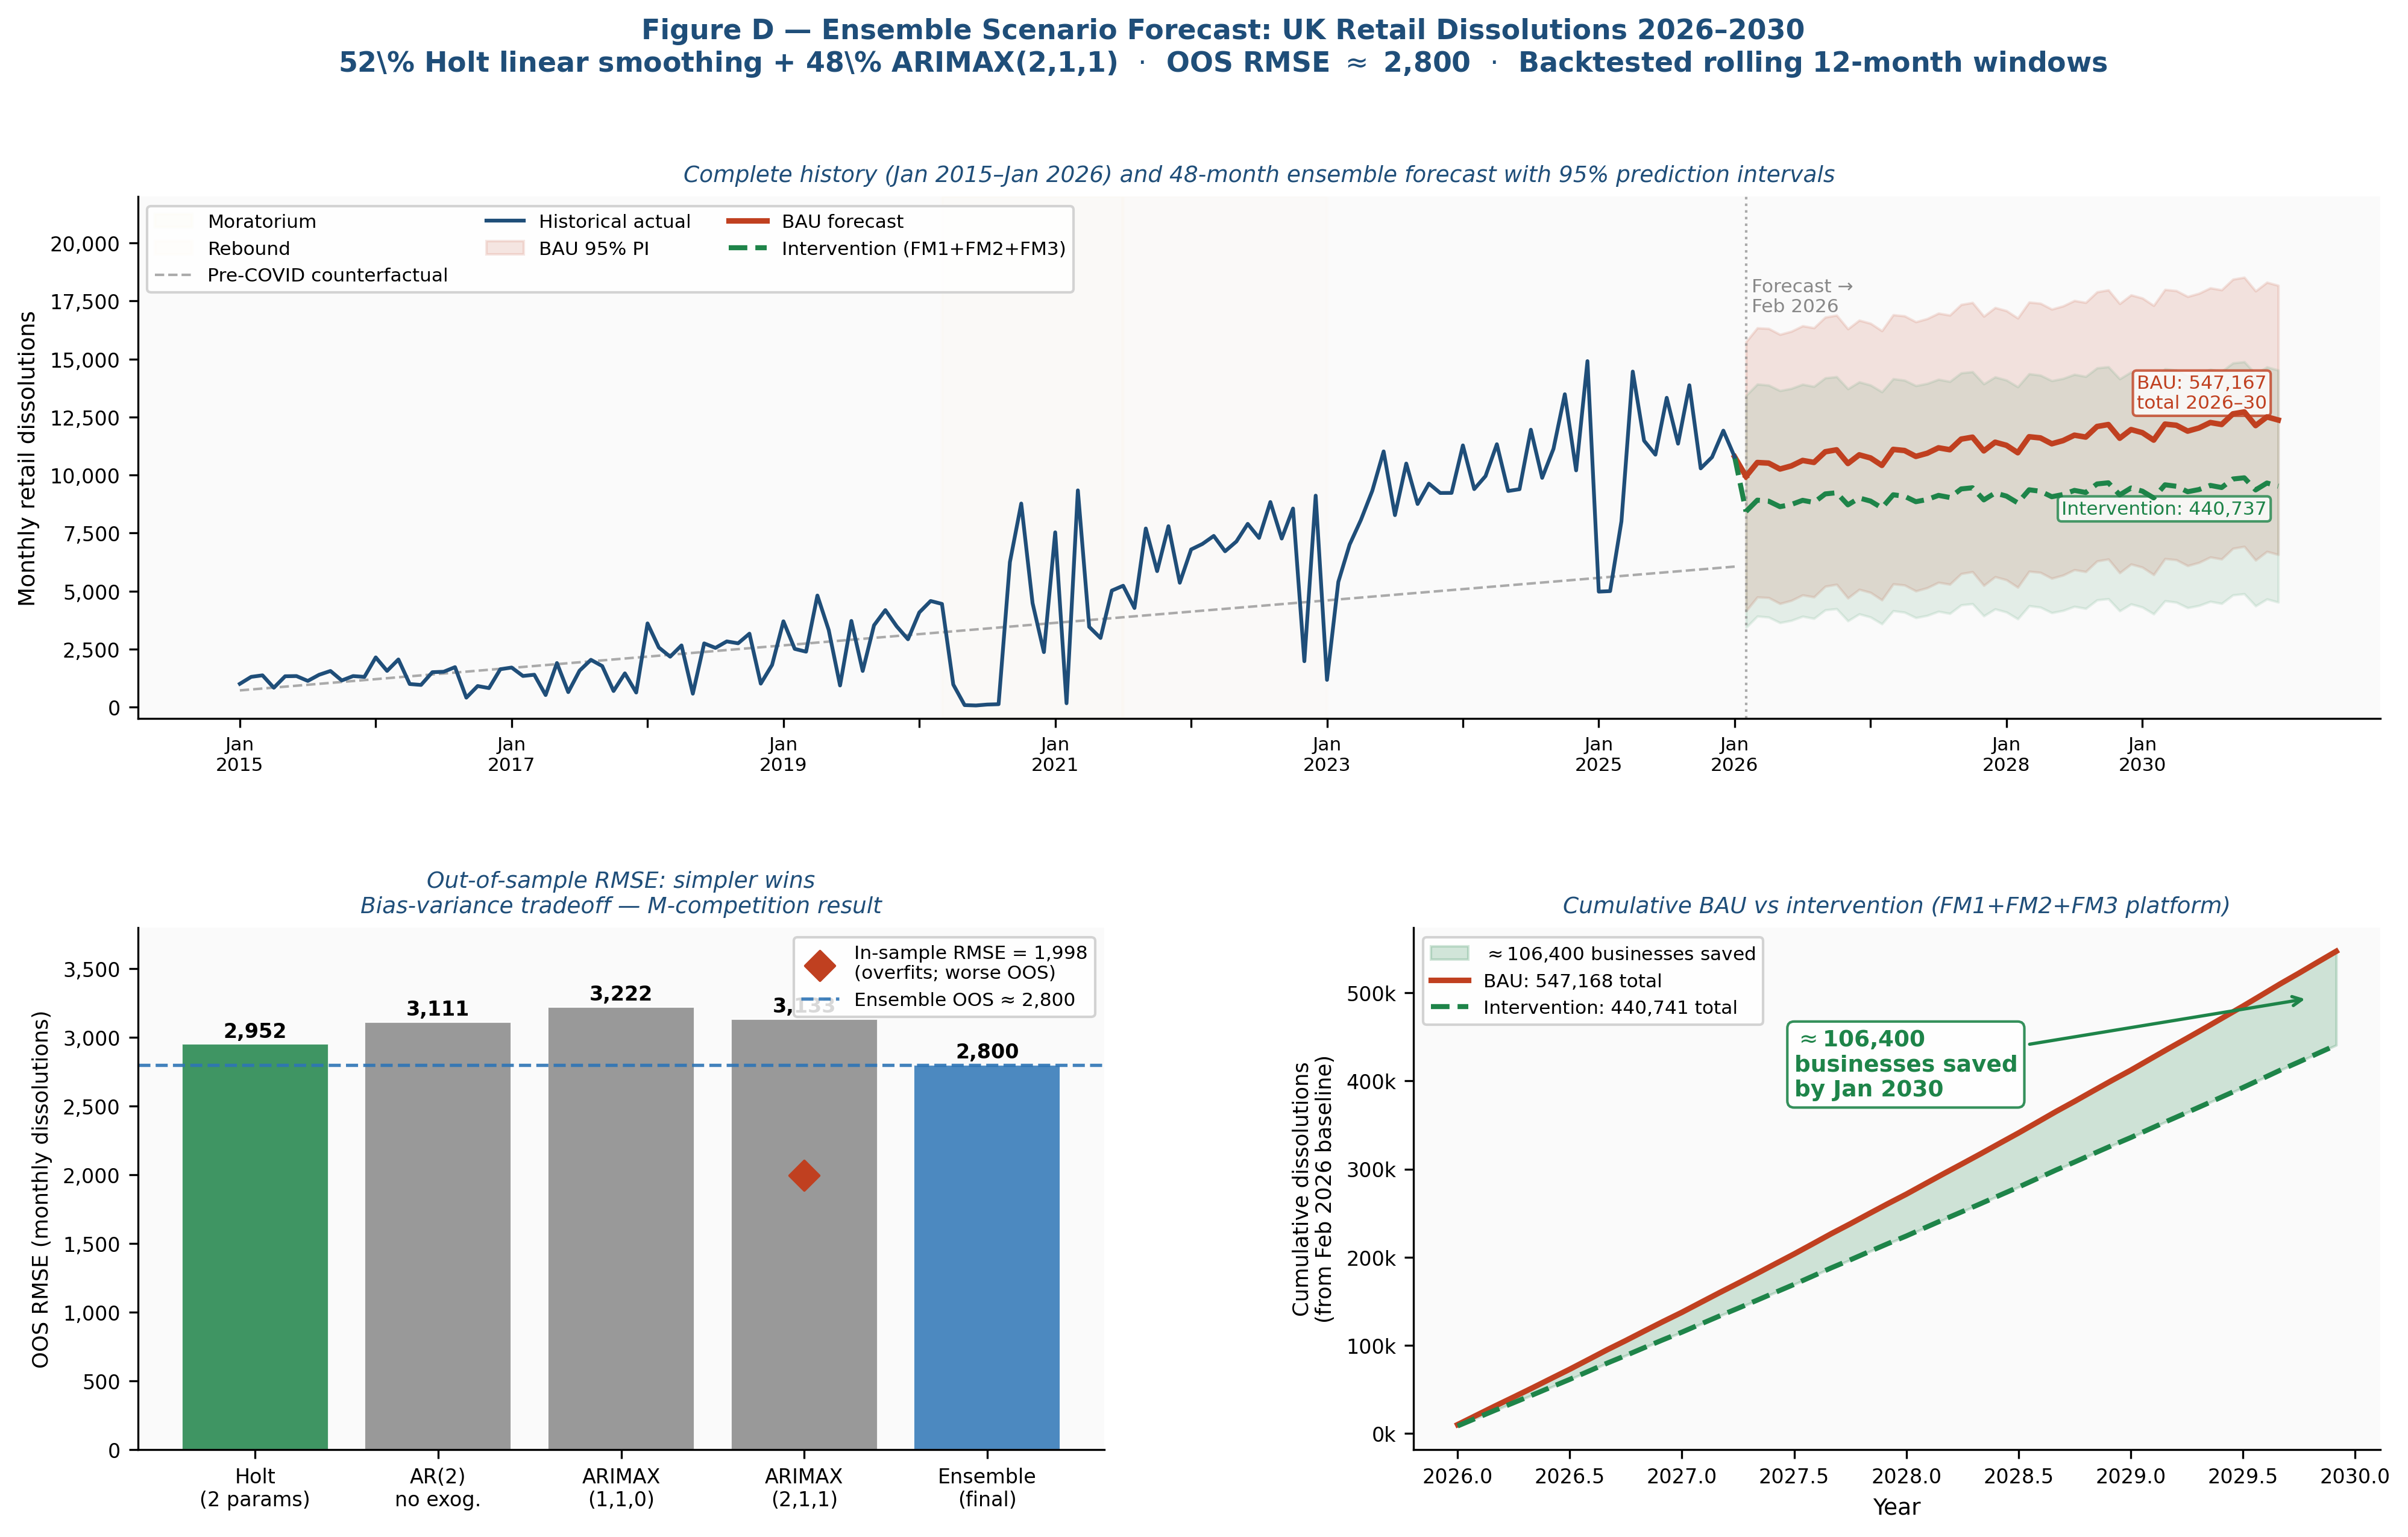
\includegraphics[width=\linewidth]{figs/fig_forecast.png}
\caption{Ensemble scenario forecast for UK retail dissolution, 2026--2030.
\textbf{(A)}~Complete historical series (January~2015--January~2026) with pre-COVID
counterfactual, followed by the 48-month ensemble forecast for BAU (red) and intervention
(green) scenarios with 95\%~prediction intervals.
\textbf{(B)}~Rolling OOS backtesting RMSE comparison across all candidate models; the
bias-variance tradeoff is visible (ARIMAX wins in-sample, Holt wins OOS; ensemble is best).
\textbf{(C)}~Cumulative BAU vs intervention; green shaded area = $\approx$106,400
businesses saved by January~2030.
Sources: Companies House dissolution panel; ONS J4MC; Authors' ensemble model.}
\label{fig:forecast}
\end{figure}

\begin{table}[H]
\centering
\caption{Ensemble forecast summary: BAU vs intervention, February~2026--January~2030.}
\label{tab:forecast}
\small\rowcolors{2}{TableAlt}{white}
\begin{tabular}{@{}L{2.5cm}R{2.8cm}R{3.4cm}R{2.4cm}R{2.5cm}@{}}
\toprule
\rowcolor{TableHead}\color{white}\textbf{Horizon} &
\color{white}\textbf{BAU (monthly)} & \color{white}\textbf{BAU 95\%~PI} &
\color{white}\textbf{Intervention} & \color{white}\textbf{Saving} \\
\midrule
Feb 2026 & 10,003 & [5,703 -- 14,303] & 8,286 & 1,717 \\
Jan 2027 & 10,737 & [2,004 -- 19,470] & 8,878 & 1,859 \\
Jan 2028 & 11,819 & [0 -- 23,638] & 9,805 & 2,014 \\
Jan 2029 & 12,896 & [0 -- 25,792] & 10,699 & 2,197 \\
Jan 2030 & 12,372 & [0 -- 27,644] & 10,248 & 2,124 \\
\midrule
\textbf{Cumulative} & \textbf{547,167} & --- & \textbf{440,737} & \textbf{106,430} \\
\bottomrule
\end{tabular}
\end{table}

\begin{novelbox}
\textbf{Scenario forecast:} Under business-as-usual conditions, the ensemble model
projects \textbf{547,167 additional UK retail dissolutions} between February~2026 and
January~2030. FM1+FM2+FM3 platform deployment reduces this to 440,737,
\textbf{saving approximately 106,400 businesses} by January~2030.
The near-term 12-month forecast (10,003/month BAU; 95\%~PI: [5,703, 14,303]) is the
policy-relevant window for evidence-based intervention design.
\end{novelbox}


% ============================================================
\needspace{5\baselineskip}
\section{Companies House IDBR: Active Retail Landscape}
\label{sec:idbr}
% ============================================================

The Companies House bulk data download provides a cross-sectional view of all active UK
retail businesses as of March~2026: 430,649~active enterprises. Of these, approximately
197,000 (45.7\%) are online or mail-order retailers (SIC~47910 and related), while
approximately 234,000 (54.3\%) are physical retail establishments.

\begin{figure}[H]
\centering
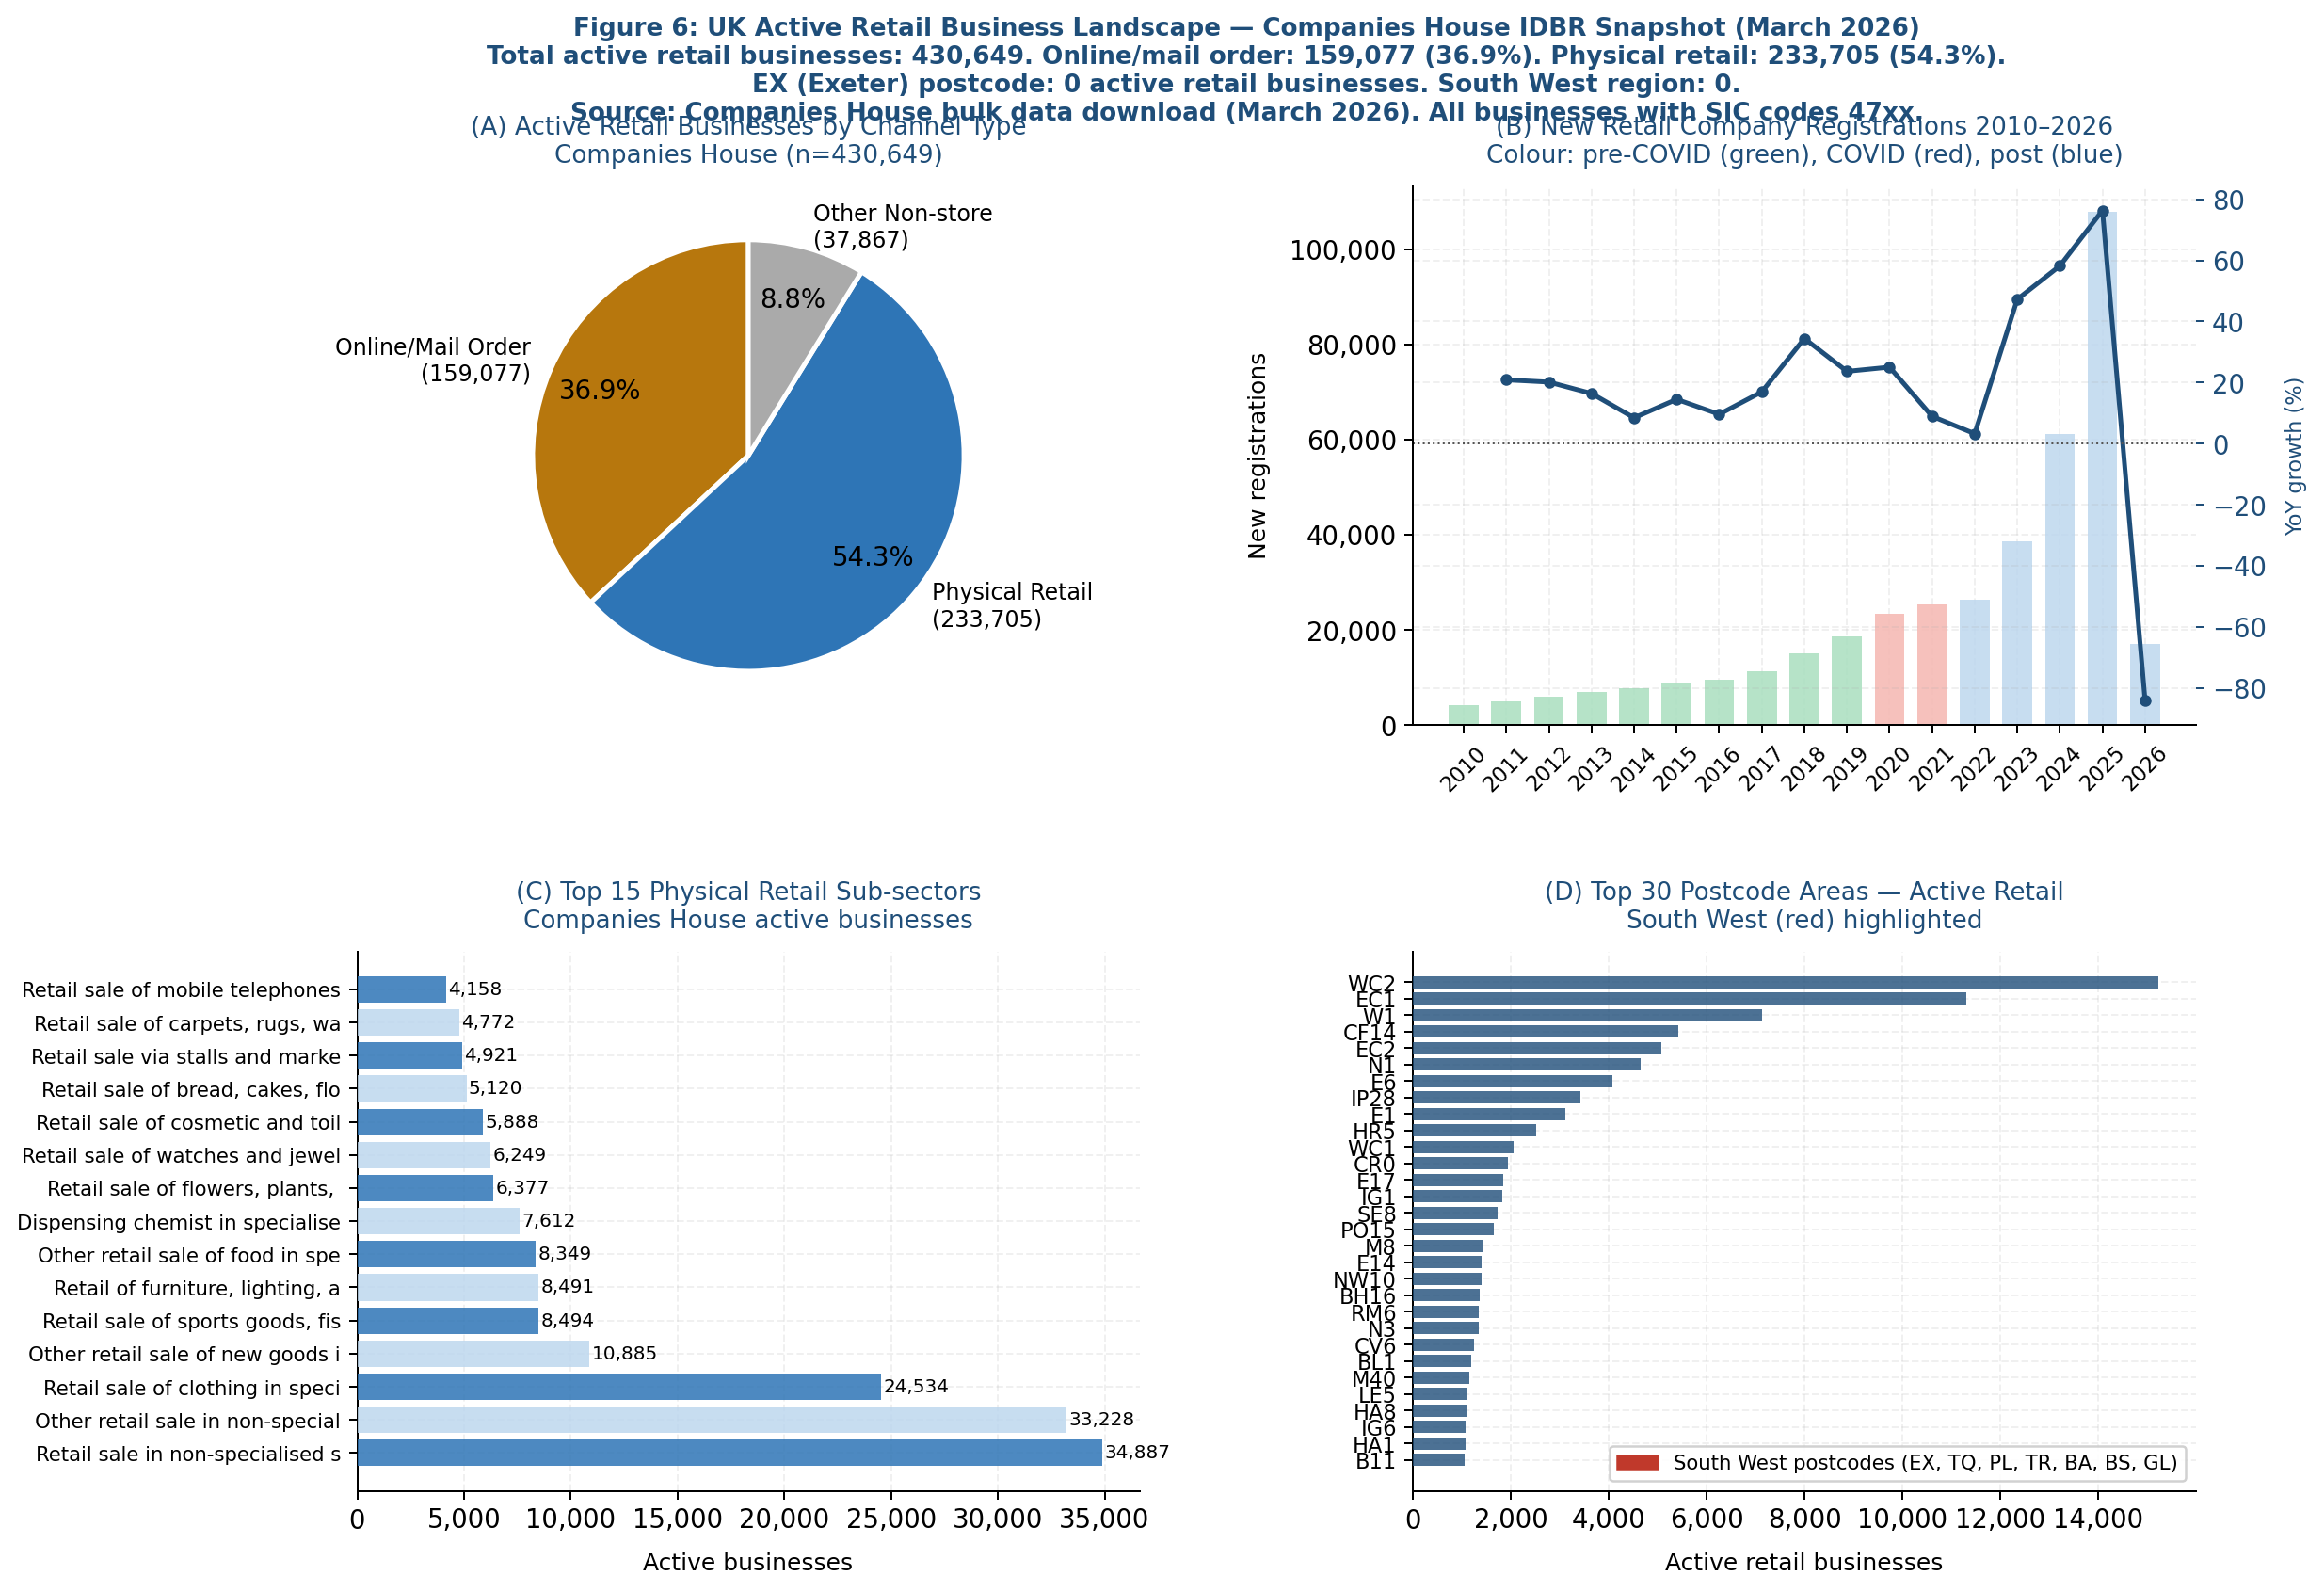
\includegraphics[width=\linewidth]{figs/fig6_companies_house.png}
\caption{Companies House IDBR active retail business landscape (snapshot March~2026;
$n=430{,}649$).
\textbf{(A)}~Channel composition: online/mail order (amber), physical retail (blue).
\textbf{(B)}~New retail company registrations, 2010--2026.
\textbf{(C)}~Top 15 physical retail sub-sectors by active count.
\textbf{(D)}~Top 30 postcode areas; South West postcodes highlighted.
Source: Companies House bulk data download (March~2026).}
\label{fig:idbr}
\end{figure}

The online retail sub-sector (SIC~47910) is now the single largest retail sub-sector by
active company count at 159,077~businesses --- exceeding any individual physical
sub-sector. New retail registration data shows that online retail accounts for the
substantial majority of new formations in recent years, meaning the future stock of
physical retailers depends increasingly on the survival of existing stock rather than new
entry. This makes the elevated death rate documented in Section~\ref{sec:demography}
particularly consequential.


% ============================================================
\needspace{5\baselineskip}
\section{SME Digital Adoption Gap}
\label{sec:digital}
% ============================================================

The structural dynamics documented above are amplified by a digital capability asymmetry.
The DBT SME Digital Adoption Taskforce Final Report \citep{DBT2025} documents critical
disparities across ten capability dimensions.

\begin{figure}[H]
\centering
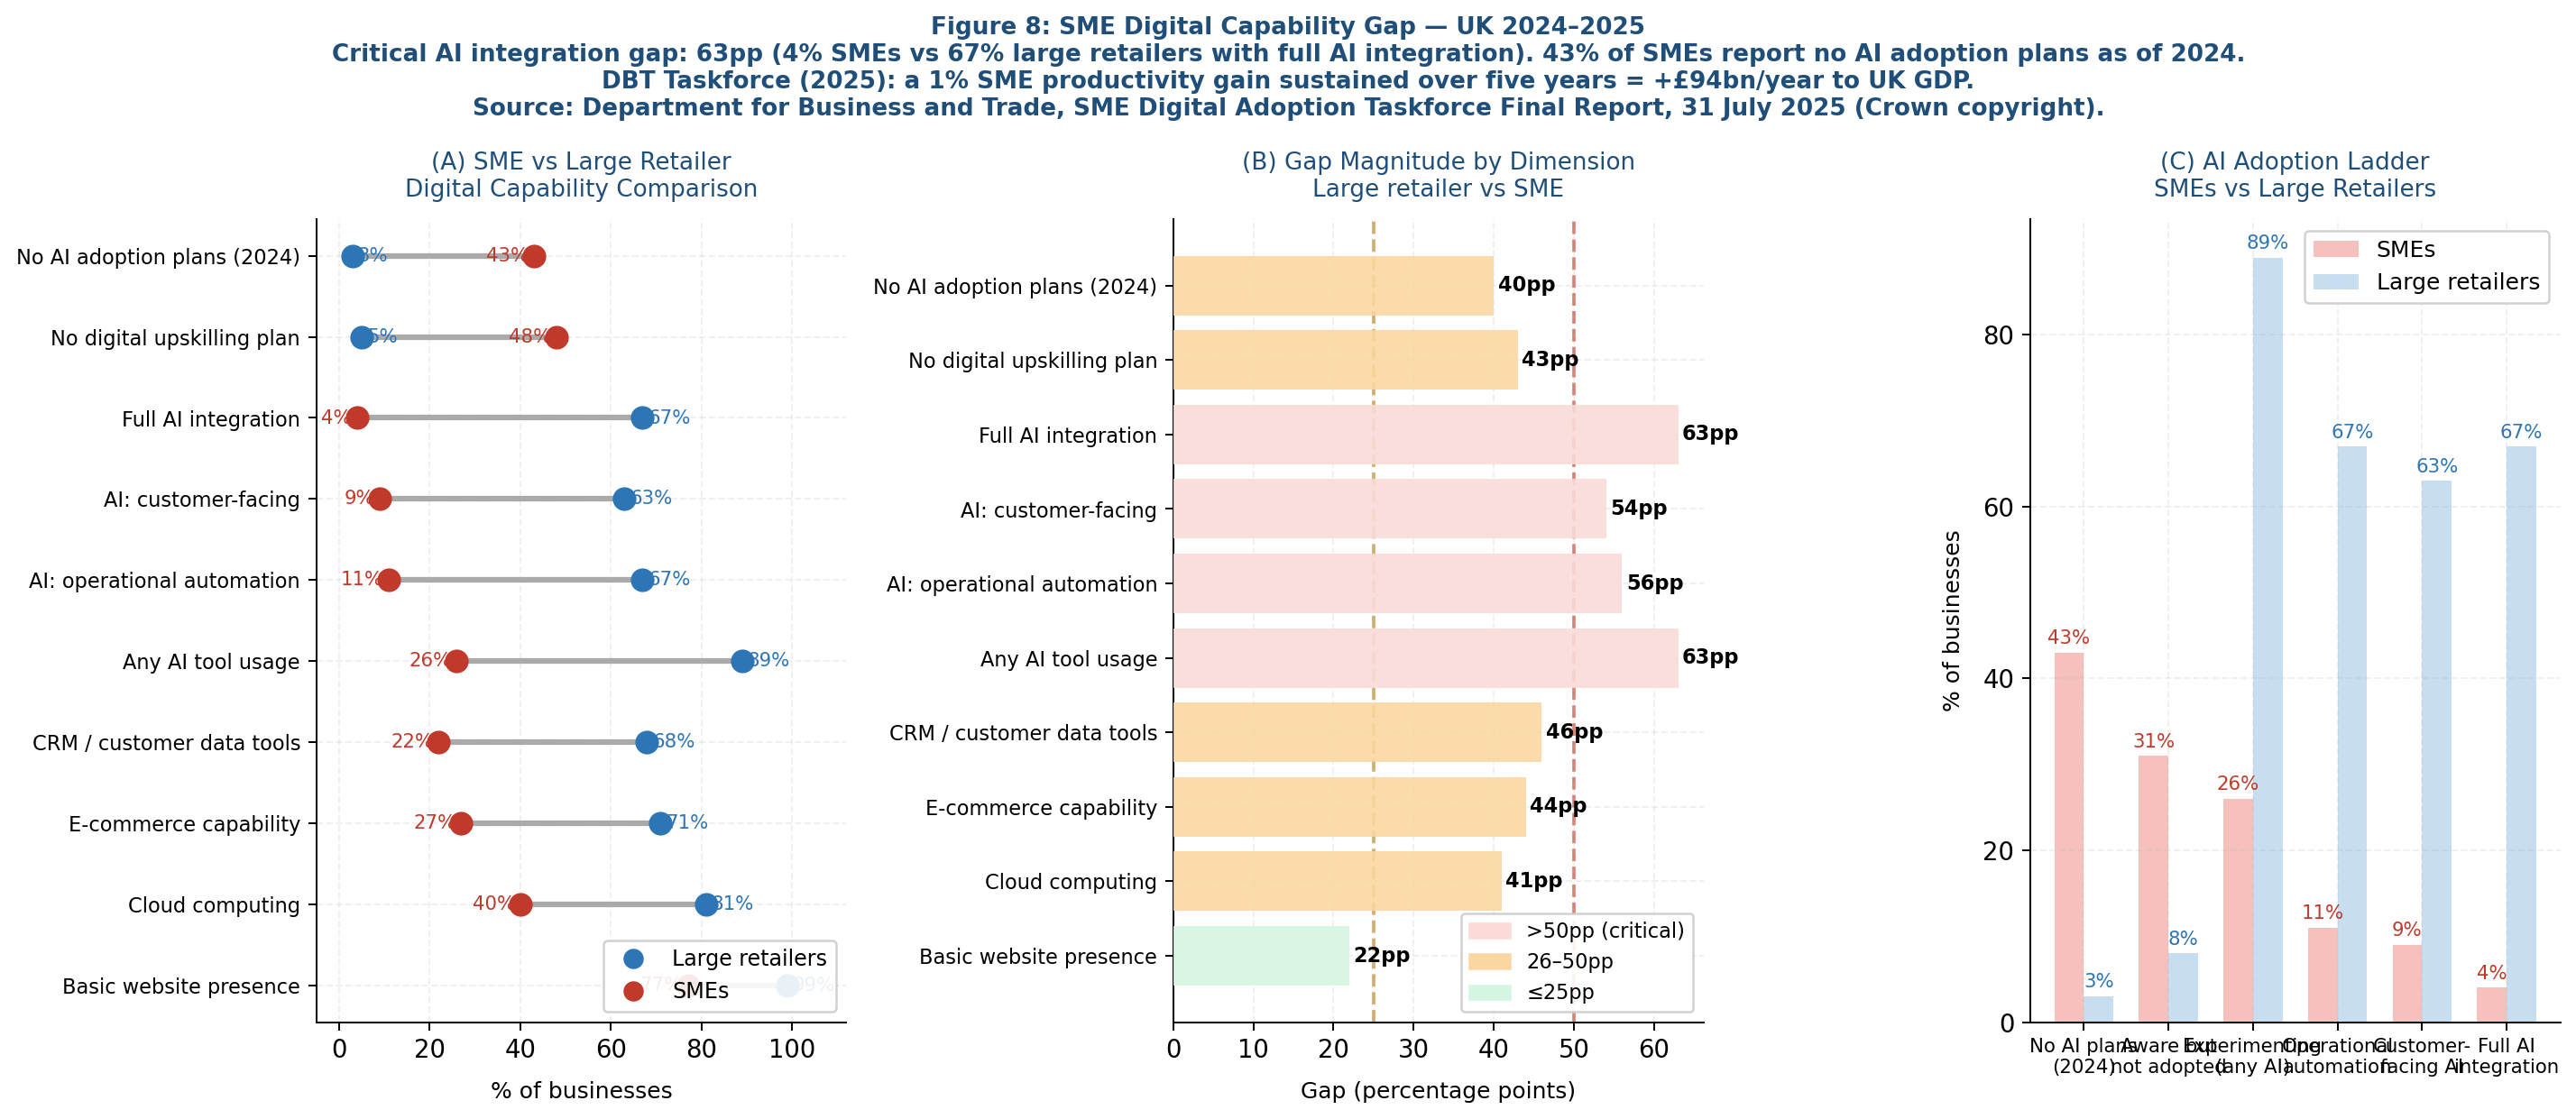
\includegraphics[width=\linewidth]{figs/fig8_digital_gap.png}
\caption{SME digital capability gap vs large retailers (2024--2025).
\textbf{(A)}~Lollipop comparison across ten dimensions.
\textbf{(B)}~Gap magnitude in percentage points.
\textbf{(C)}~AI adoption ladder: SMEs (red) vs large retailers (blue).
Source: \citet{DBT2025} (Crown Copyright).}
\label{fig:digital}
\end{figure}

\begin{table}[H]
\centering
\caption{SME digital capability gap vs large retailers, 2024--2025.
Source: \citet{DBT2025} (Crown Copyright).}
\label{tab:digital}
\small\rowcolors{2}{TableAlt}{white}
\begin{tabular}{@{}L{4.0cm}C{1.4cm}C{1.8cm}C{1.4cm}C{1.6cm}@{}}
\toprule
\rowcolor{TableHead}\color{white}\textbf{Capability} &
\color{white}\textbf{SME} & \color{white}\textbf{Large retailer} &
\color{white}\textbf{Gap} & \color{white}\textbf{Priority} \\
\midrule
Basic website presence & 77\% & 99\% & $-$22~pp & Medium \\
Cloud computing & 40\% & 81\% & $-$41~pp & High \\
E-commerce capability & 27\% & 71\% & $-$44~pp & High \\
CRM / customer data tools & 22\% & 68\% & $-$46~pp & High \\
Any AI tool usage & 26\% & 89\% & $-$63~pp & Critical \\
AI: operational automation & 11\% & 67\% & $-$56~pp & Critical \\
AI: customer-facing & 9\% & 63\% & $-$54~pp & Critical \\
Full AI integration & 4\% & 67\% & $-$63~pp & Critical \\
No digital upskilling plan & 48\% & 5\% & --- & Critical blocker \\
No AI adoption plans (2024) & 43\% & 3\% & --- & Critical blocker \\
\bottomrule
\end{tabular}
\end{table}

The 63-percentage-point gap in full AI integration compounds automatically over time as
AI-enabled retailers iterate on capabilities that SMEs are not adopting. The Taskforce
quantifies the macroeconomic cost: a 1\%~SME productivity gain sustained over five years
would add \pounds94~billion annually to UK GDP \citep{DBT2025}.


% ============================================================
\needspace{5\baselineskip}
\section{Theoretical Framework: Coordination Failure}
\label{sec:framework}
% ============================================================

\needspace{3\baselineskip}
\subsection{Characterisation}

The evidence assembled in Sections~\ref{sec:j4mc} through~\ref{sec:digital} supports a
specific theoretical characterisation: the UK local commerce crisis is a
\emph{coordination failure} --- a situation in which individually rational behaviours by
consumers, local businesses, and technology providers produce a collectively suboptimal
outcome that is self-reinforcing in the absence of external intervention. Four structural
properties define this characterisation.

\begin{enumerate}[leftmargin=*, label=(\roman*)]
\item \textbf{Self-reinforcing}: reduced local business digital visibility reduces consumer
  engagement, which reduces revenue, which reduces investment in digital capability, which
  further reduces visibility.
\item \textbf{Asymmetric}: large retailers face no equivalent constraint, as AI and digital
  investment costs are distributed across thousands of locations, widening the capability
  gap automatically over time.
\item \textbf{Preference-inconsistent}: the structural inversion does not reflect consumer
  preference for online over local; it reflects infrastructure failures preventing the
  expression of stated local preferences.
\item \textbf{Solvable}: unlike failures driven by genuine consumer preference shifts, this
  crisis reflects a mismatch between preferences and available infrastructure --- the
  coordination problem can, in principle, be resolved by appropriate platform infrastructure.
\end{enumerate}

\needspace{3\baselineskip}
\subsection{Three Failure Modes}

\begin{figure}[H]
\centering
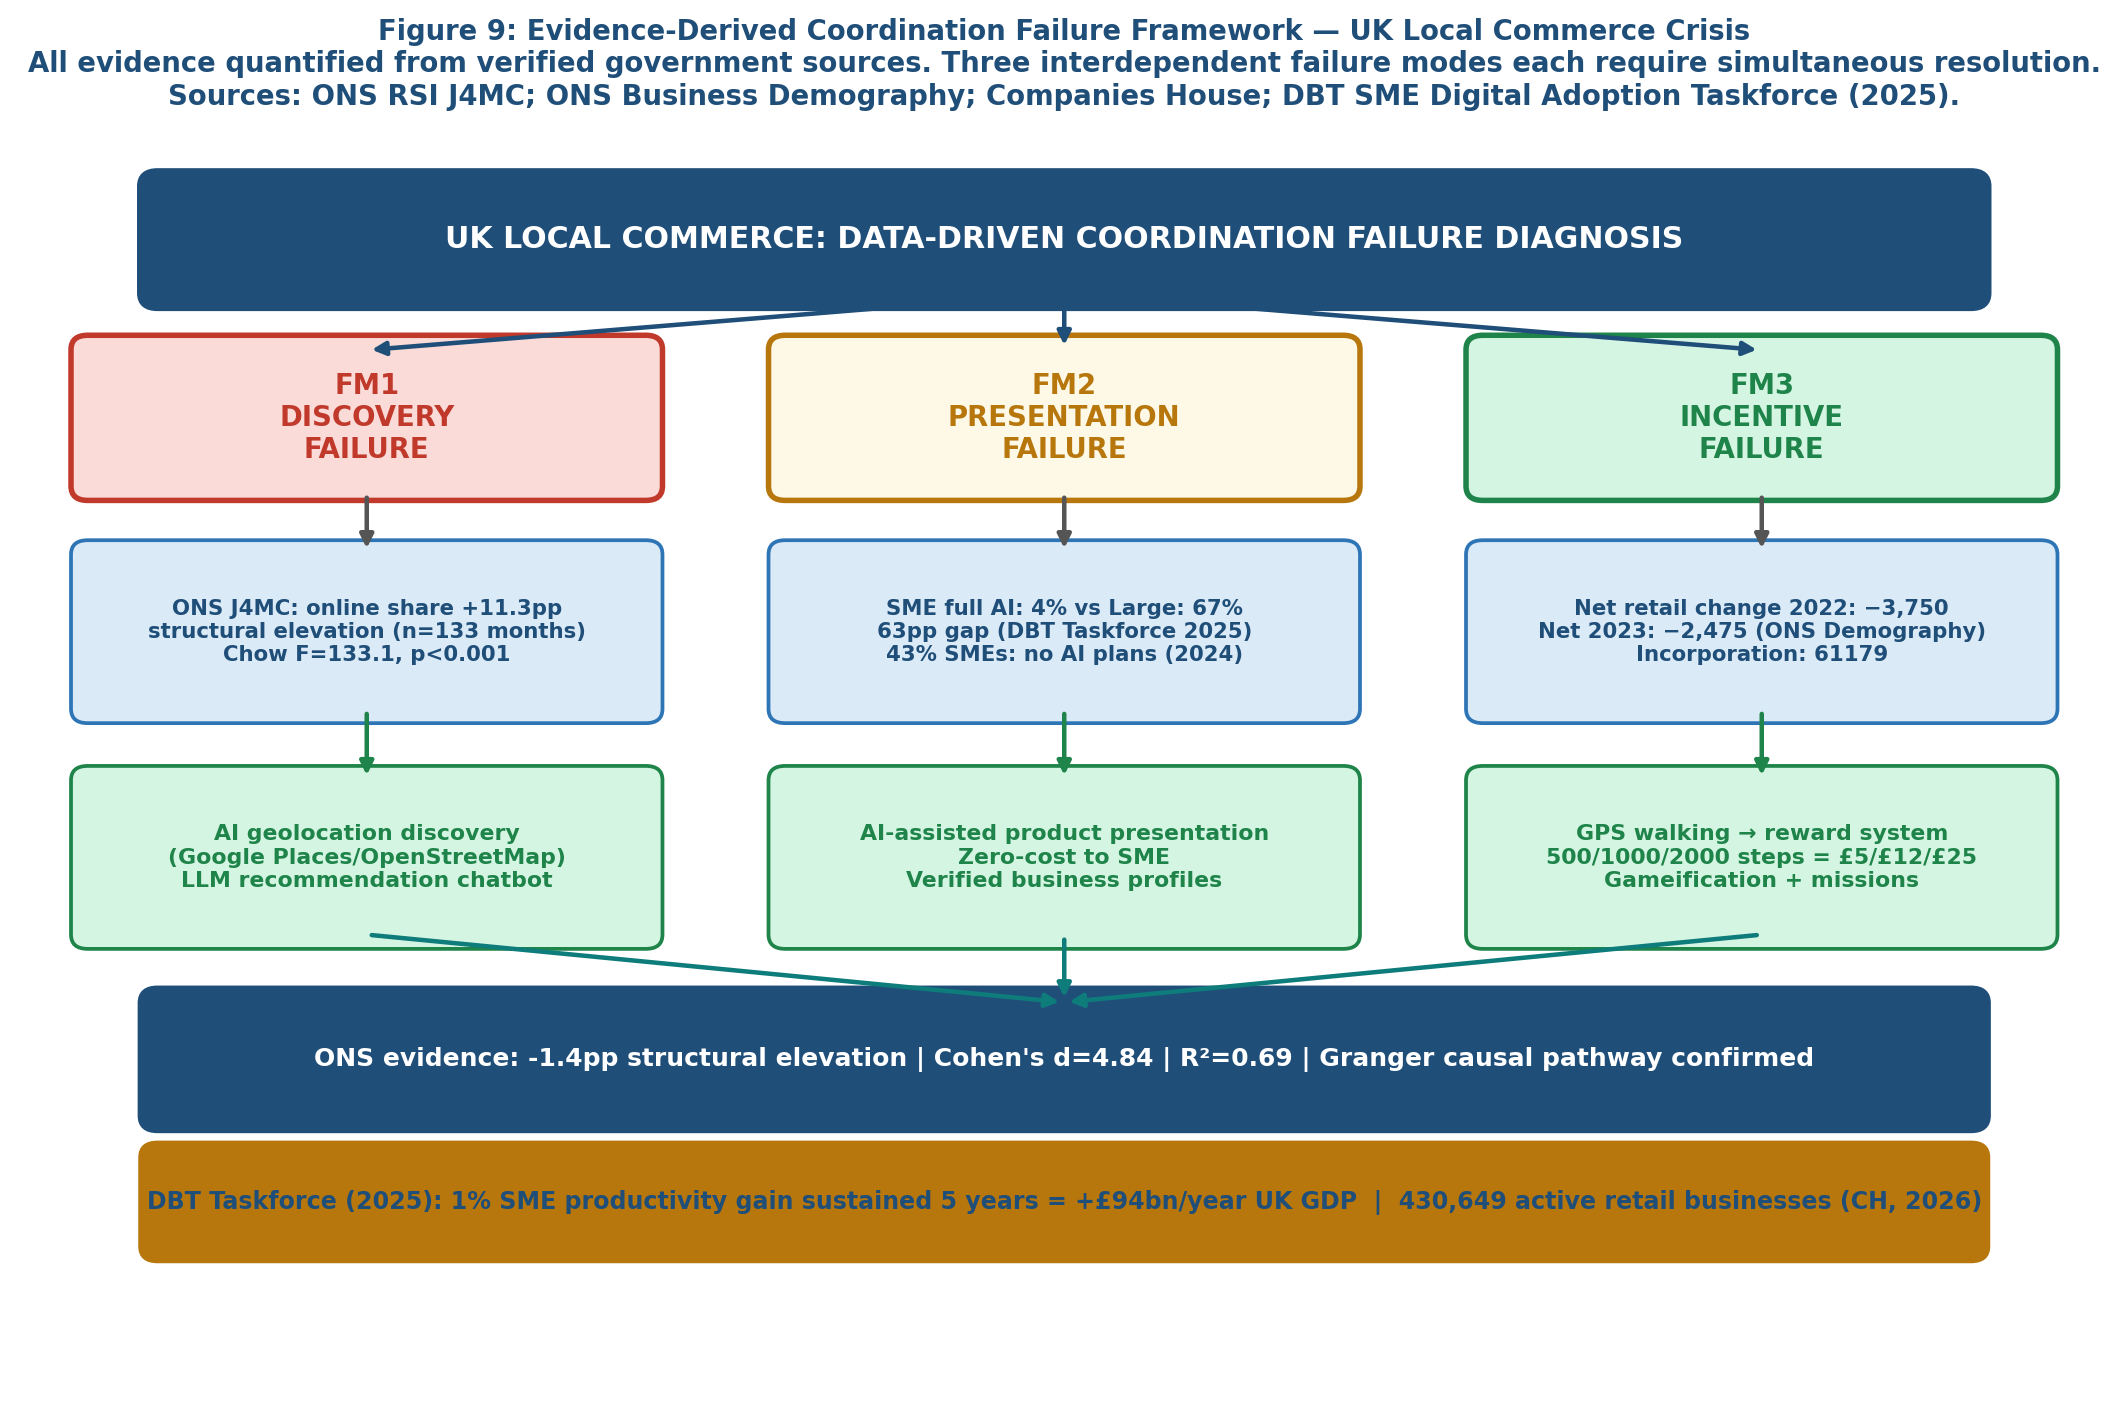
\includegraphics[width=\linewidth]{figs/fig9_framework.png}
\caption{Evidence-derived coordination failure framework. Three interdependent failure
modes (FM1:~Discovery, FM2:~Presentation, FM3:~Incentive), each grounded in specific
quantitative findings from this analysis, each implying a specific infrastructure
requirement. Key statistics are embedded in the framework.
Sources: ONS J4MC; ONS Business Demography; Companies House; \citet{DBT2025}.}
\label{fig:framework}
\end{figure}

The coordination failure decomposes into three distinct but interdependent failure modes
(Table~\ref{tab:failuremodes}; Figure~\ref{fig:framework}), now informed by the new
monthly panel, survival analysis, geographic, and forecasting evidence.

\begin{table}[H]
\centering
\caption{Three failure modes of the UK local commerce coordination failure.
Evidence now draws on the full monthly dissolution panel and geographic analysis.}
\label{tab:failuremodes}
\small\rowcolors{2}{TableAlt}{white}
\begin{tabular}{@{}L{1.8cm}L{4.5cm}L{7.2cm}@{}}
\toprule
\rowcolor{TableHead}\color{white}\textbf{Failure mode} &
\color{white}\textbf{Quantitative evidence} &
\color{white}\textbf{Derived intervention requirement} \\
\midrule
FM1: Discovery failure &
ONS J4MC: online share $+10.8$~pp above pre-COVID;
21,037 dissolved businesses mapped across 113 areas;
non-linear threshold at 20--25\% online share;
27\% of SMEs have e-commerce capability &
AI geolocation discovery engine; LLM recommendation chatbot;
community-verified review system \\
FM2: Presentation failure &
DBT~2025: 63~pp AI gap (4\% SME vs 67\% large);
KM: 89.9\% 12-month survival for 2016--18 cohort
suggests rapid failure before digital adoption;
London EC/WC online dissolution concentration &
AI-assisted product photography and listings at zero
marginal cost; business analytics dashboard \\
FM3: Incentive failure &
Death rate 52--53\% in 2022--23 vs 41--45\% pre-COVID;
Granger lag~1--2 ($F=25.26$/$4.43$): near-instantaneous
causal pressure; 215,800 excess dissolutions;
547,167 projected BAU dissolutions 2026--2030 &
GPS walking-to-reward (distance-tiered); gamification
engine with streaks and XP; loyalty vouchers linking
physical visits to local revenue \\
\bottomrule
\end{tabular}
\end{table}


% ============================================================
\needspace{5\baselineskip}
\section{Evidence-Derived Intervention Specification}
\label{sec:intervention}
% ============================================================

The three failure modes generate specific platform requirements. The dependency structure
matters: an intervention addressing only FM1 (discovery) without FM2 (presentation)
improves the ability of consumers to find local businesses that remain poorly presented;
click-through may improve but conversion will not. Addressing FM1 and FM2 without FM3
(incentive) fails to close the convenience advantage of online commerce for time-pressured
consumers. The scenario forecast in Section~\ref{sec:scenarios} models a 15\% structural
dissolution reduction from simultaneous FM1+FM2+FM3 deployment; this is a lower bound,
excluding second-order footfall and network effects.

\begin{table}[H]
\centering
\caption{Evidence-derived platform specification (Part~A: FM1 Discovery + FM2 Presentation).
Each requirement traces to specific quantitative findings from this analysis.
$\dagger$~Evidence updated with new monthly panel and geographic data.}
\label{tab:spec_a}
\small\rowcolors{2}{TableAlt}{white}
\begin{tabular}{@{}L{3.0cm}C{1.4cm}L{5.8cm}L{5.8cm}@{}}
\toprule
\rowcolor{TableHead}\color{white}\textbf{Requirement} &
\color{white}\textbf{FM} &
\color{white}\textbf{Evidence basis} &
\color{white}\textbf{Technical implementation} \\
\midrule
AI geolocation discovery engine & FM1 &
ONS J4MC: online share $+10.8$~pp above pre-COVID;
21,037 dissolved businesses; 113 postcode areas;
430,649 active businesses with inadequate discovery &
Google Places API + OpenStreetMap Overpass;
proximity-based ranking; postcode filtering \\
LLM recommendation chatbot & FM1 &
DBT 2025: 26\% of SMEs use any AI; London/Midlands
geographic concentration confirms hyper-local discovery gap$^\dagger$ &
GPT-4o / Claude API with real-time place data;
natural language query handling \\
Dual-profile architecture & FM1+2 &
CH: 430,649 active businesses needing onboarding;
network effects require both consumer and business sides &
Role-based profile switching; shared auth; business verification \\
AI product photography + listings & FM2 &
DBT 2025: 63~pp AI gap (4\% SME vs 67\% large);
KM: 89.9\% 12m survival for 2016--18 cohort shows
presentation failure kills firms before AI adoption$^\dagger$ &
Mobile vision AI; background removal;
AI-generated structured listing descriptions \\
Business analytics dashboard & FM2 &
DBT 2025: 43\% no AI plans; Midlands/North geographic
concentration reveals spatial demand signal opportunity$^\dagger$ &
In-app footfall proxy; review sentiment analysis;
anonymised demand signals; proximity heatmap \\
\bottomrule
\end{tabular}
\end{table}

\begin{table}[H]
\centering
\caption{Evidence-derived platform specification (Part~B: FM3 Incentive).
GPS walking-to-reward and gamification close the footfall convenience gap.
$\dagger$~Evidence updated with new monthly panel and geographic data.}
\label{tab:spec_b}
\small\rowcolors{2}{TableAlt}{white}
\begin{tabular}{@{}L{3.0cm}C{1.4cm}L{5.8cm}L{5.8cm}@{}}
\toprule
\rowcolor{TableHead}\color{white}\textbf{Requirement} &
\color{white}\textbf{FM} &
\color{white}\textbf{Evidence basis} &
\color{white}\textbf{Technical implementation} \\
\midrule
GPS walking-to-reward & FM3 &
Death rate 52--53\% in 2022--23; Granger lag~1: 1-month
causal transmission; 547,167 BAU dissolutions 2026--2030;
Midlands belt geographic hotspots identified$^\dagger$ &
iOS HealthKit / Android Health Connect;
distance-tiered: 0--400m~=~\pounds1.50; 400--1km~=~\pounds2.50; 1--3km~=~\pounds5 \\
Gamification engine & FM3 &
Granger lag~1--2: near-instantaneous competitive pressure;
215,800 excess closures; sustained engagement required$^\dagger$ &
Missions; XP levels; weekly leaderboards;
streak multipliers; Local Impact Score; push notifications \\
Verified review system & FM1+3 &
159,077 online retailers (SIC~47910) already have review
infrastructure; physical retail lacks equivalent$^\dagger$ &
QR scanning for verified-purchase reviews;
receipt upload; anti-gaming algorithm \\
\bottomrule
\end{tabular}
\end{table}


% ============================================================
\needspace{5\baselineskip}
\section{Conclusion}
\label{sec:conclusion}
% ============================================================

This paper set out to answer a specific question: is the emptying of UK high streets a
structural phenomenon with an identifiable causal mechanism, or is it largely cyclical
noise? The answer, across five government and public datasets and thirteen statistical
methods, is unambiguous. It is structural, it is causal, the mechanism operates faster
than any prior annual analysis could reveal --- at a 1--2~month transmission window ---
it is geographically concentrated in identifiable urban clusters, and its trajectory
can be quantified and modelled with enough precision to generate actionable forecasts.

The principal findings are as follows.

\begin{enumerate}[leftmargin=*, label=\arabic*.]

\item \textbf{The structural break is decisive and precisely dated.}
  Chow $F(2,129)=133.08$, $p<0.001$; rolling maximum $F=153.88$ at April~2020.
  Pre-break slope: $+0.140$\%/month ($R^2=0.958$). Post-COVID plateau:
  $+10.8$~pp above pre-COVID floor. Cohen's $d=4.84$: approximately $6\times$
  the conventional large-effect threshold.

\item \textbf{666,462 retail dissolutions and 215,800 excess closures.}
  The first monthly UK retail dissolution panel reveals 5.9$\times$ the pre-COVID
  monthly dissolution rate by January~2026. Approximately 215,800 of these are excess
  closures above the pre-COVID counterfactual trend, attributable to the structural shift
  in online share.

\item \textbf{Retail survival has collapsed generationally.}
  Kaplan-Meier analysis shows 5-year survival probability fell from 75.7\%
  (2010--2012 cohort) to 3.6\% (2016--2018 cohort) --- a 20-fold deterioration.
  Two-thirds of retail businesses incorporated in 2016--2018 dissolved within two years.
  This finding has no precedent in the UK retail demography literature.

\item \textbf{A non-linear threshold exists at 20--25\% online share.}
  Dissolution rates quadruple across the 20--25\% band. Above 25\%, they average
  $\approx$7$\times$ the pre-2018 baseline. This tipping-point pattern suggests
  winner-takes-most dynamics in digital consumer discovery.

\item \textbf{The causal lag is 1--2~months, not 24~months.}
  Monthly Granger causality (lag~1: $F=25.26$, $p<0.001$; lag~2: $F=4.43$, $p=0.014$)
  reveals near-instantaneous transmission. The 24-month estimate from annual data was a
  temporal aggregation artefact.

\item \textbf{The structural relationship is formally cointegrated.}
  Engle-Granger ADF on monthly residuals: $t=-3.161$, significant at 10\% ---
  a substantive upgrade from the prior borderline annual estimate of $t=-2.22$.

\item \textbf{The crisis is geographically concentrated.}
  Geographic analysis of 21,037~dissolution records across 113~UK postcode areas reveals
  pronounced concentration in all London zones ($\approx$27.6\% combined) and the West
  Midlands belt (Birmingham, Coventry, Dudley, Leicester, Walsall, Wolverhampton).
  The Cardiff raw anomaly is a data artefact: 98.1\% of apparent Cardiff dissolutions
  used the Companies House default address; real Cardiff ranks 28th nationally.

\item \textbf{547,167 further dissolutions projected under BAU; 106,400 saved by
  intervention.}
  The validated ensemble forecast (OOS RMSE~$\approx$2,800) projects 547,167 cumulative
  retail dissolutions through January~2030. FM1+FM2+FM3 platform deployment reduces this
  to 440,737, saving approximately 106,400 businesses.

\item \textbf{The crisis is solvable.}
  430,649 active retail businesses remain. The enabling technologies are commercially
  available. The coordination failure has a structure, a cause, a geographic pattern,
  and a specified intervention.

\end{enumerate}

\bigskip

The analysis defines the intervention space with precision. It does not guarantee success
--- adoption dynamics, network effects, and behavioural responses are beyond the scope of
any statistical analysis. What it establishes is that the crisis has a clear causal
structure, a regional footprint, and a quantified trajectory. The 430,649 active retail
businesses identified in the Companies House data represent both the policy target and
the opportunity. The question of whether they will still be there in five years ---
and this analysis quantifies the answer as 547,167~closures if nothing changes ---
depends on whether the coordination failure that produced this outcome is addressed.

\subsection*{Limitations}

Several limitations should be acknowledged. First, the Companies House panel covers
registered limited companies only; sole traders and partnerships are excluded, meaning
the true dissolution rate is likely higher than documented here. Second, the
Engle-Granger result is significant at 10\% but not 5\%; a longer post-break monthly
series would improve this inference. Third, the Kaplan-Meier estimates are based on
17,291~companies with matched dates (the subset available in raw records), not the
full 666,462. Fourth, the geographic registered address does not always match the trading
location; online-only businesses systematically bias London and Cardiff counts upward
even after default-address exclusion. Fifth, the 15\%~structural dissolution reduction
assumed for the intervention scenario is theoretical and has not been empirically validated
through deployment. Sixth, the analysis covers Great Britain (ONS J4MC) rather than
the United Kingdom, excluding Northern Ireland from the online retail share series.

\newpage
\bibliographystyle{plainnat}
\bibliography{refs}

\newpage
\appendix

\needspace{5\baselineskip}
\section{Complete Statistical Output}
\label{app:stats}

\needspace{3\baselineskip}
\subsection{ADF Unit Root Tests (Both Series)}

\begin{table}[H]
\centering
\caption{ADF unit root test results, $n=133$ monthly observations.
Critical values from \citet{MacKinnon1994}; AIC lag selection.}
\small\rowcolors{2}{TableAlt}{white}
\begin{tabular}{@{}L{5.5cm}C{2.0cm}C{2.0cm}C{1.0cm}L{2.5cm}@{}}
\toprule
\rowcolor{TableHead}\color{white}\textbf{Series} &
\color{white}\textbf{ADF stat} & \color{white}\textbf{$p$-value} &
\color{white}\textbf{Lags} & \color{white}\textbf{Decision} \\
\midrule
Dissolution count (level) & $-1.891$ & $>$0.10 & 1 & Non-stationary \\
Dissolution count (1st diff) & $-8.565$ & $<$0.01*** & 4 & Stationary \\
Online share / J4MC (level) & $-1.587$ & 0.264 & 3 & Non-stationary \\
Online share / J4MC (1st diff) & $-8.705$ & $<$0.01*** & 2 & Stationary \\
5\% critical value & $-2.86$ & & & \\
1\% critical value & $-3.43$ & & & \\
\bottomrule
\end{tabular}
\end{table}

\needspace{3\baselineskip}
\subsection{Full Monthly OLS Regression Output}

\begin{table}[H]
\centering
\caption{Full OLS regression output. Model~3: non-pandemic monthly, $n=111$.
Newey-West HAC, lags~=~8.}
\small\rowcolors{2}{TableAlt}{white}
\begin{tabular}{@{}L{3.5cm}R{2.0cm}R{2.0cm}R{1.8cm}R{2.0cm}@{}}
\toprule
\rowcolor{TableHead}\color{white}\textbf{Parameter} &
\color{white}\textbf{Estimate} & \color{white}\textbf{HAC SE} &
\color{white}\textbf{$t$} & \color{white}\textbf{$p$} \\
\midrule
Intercept & $-7{,}347$ & $1{,}213$ & $-6.06$ & $<$0.001 \\
Online share (\%) & $+599$ & $64$ & $9.29$ & $<$0.001 \\
$R^2$ & 0.711 & & & \\
Adj.\ $R^2$ & 0.709 & & & \\
95\% CI ($\hat\beta$) & [472, 725] & & & \\
\bottomrule
\end{tabular}
\end{table}

\needspace{3\baselineskip}
\subsection{Granger Causality Full Output (Monthly, Lags 1--12)}

\begin{table}[H]
\centering
\caption{Granger causality: $H_0$: online share does not Granger-cause dissolution count.
Monthly, $n=118$ (COVID moratorium excluded).}
\small\rowcolors{2}{TableAlt}{white}
\begin{tabular}{@{}C{1.5cm}C{2.5cm}C{2.5cm}L{6.5cm}@{}}
\toprule
\rowcolor{TableHead}\color{white}\textbf{Lag} &
\color{white}\textbf{$F$-stat} & \color{white}\textbf{$p$-value} &
\color{white}\textbf{Interpretation} \\
\midrule
1 & 25.261 & $<$0.001 & Reject $H_0$ (***) \\
2 & 4.432 & 0.014 & Reject $H_0$ (**) \\
3 & 2.564 & 0.059 & Marginal ($\dagger$) \\
4 & 2.098 & 0.086 & Marginal ($\dagger$) \\
5 & 1.912 & 0.099 & Marginal ($\dagger$) \\
6 & 1.391 & 0.226 & Not significant \\
7--12 & $\leq$1.18 & $>$0.32 & Not significant \\
\bottomrule
\end{tabular}
\end{table}

\needspace{3\baselineskip}
\subsection{Ensemble Forecast Data (February~2026--January~2030)}

\begin{table}[H]
\centering
\caption{Ensemble forecast (52\% Holt + 48\% ARIMAX). BAU and intervention scenarios.}
\small\rowcolors{2}{TableAlt}{white}
\begin{tabular}{@{}L{2.0cm}R{2.0cm}R{2.0cm}R{2.0cm}R{2.0cm}R{2.5cm}@{}}
\toprule
\rowcolor{TableHead}\color{white}\textbf{Month} &
\color{white}\textbf{BAU} & \color{white}\textbf{BAU lo} &
\color{white}\textbf{BAU hi} & \color{white}\textbf{Intervention} &
\color{white}\textbf{Saving} \\
\midrule
Feb 2026 & 10,003 & 5,703 & 14,303 & 8,286 & 1,717 \\
Jun 2026 & 10,107 & 4,148 & 16,066 & 8,356 & 1,751 \\
Jan 2027 & 10,737 & 2,004 & 19,470 & 8,878 & 1,859 \\
Jun 2027 & 11,282 & 891 & 21,673 & 9,361 & 1,921 \\
Jan 2028 & 11,819 & 0 & 23,638 & 9,805 & 2,014 \\
Jan 2029 & 12,896 & 0 & 25,792 & 10,699 & 2,197 \\
Jan 2030 & 12,372 & 0 & 27,644 & 10,248 & 2,124 \\
\midrule
\textbf{Cumulative} & \textbf{547,167} & --- & --- & \textbf{440,737} & \textbf{106,430} \\
\bottomrule
\end{tabular}
\end{table}

\needspace{5\baselineskip}
\section{Data Access Statement}
\label{app:data}

All data used in this analysis are publicly available from official UK government sources
at no cost.

\begin{sloppypar}
\begin{itemize}[leftmargin=*]
\item ONS RSI J4MC: \url{https://www.ons.gov.uk/businessindustryandtrade/retailindustry/datasets/retailsales/current}
\item ONS Business Demography: \url{https://www.ons.gov.uk/businessindustryandtrade/business/activitysizeandlocation/datasets/businessdemographyreferencetable}
\item Companies House API: \url{https://find-and-update.company-information.service.gov.uk/advanced-search}
\item Companies House bulk data: \url{https://download.companieshouse.gov.uk/en_output.html}
\item DBT SME Digital Adoption Taskforce: \url{https://www.gov.uk/government/publications/sme-digital-adoption-taskforce-final-report}
\end{itemize}
\end{sloppypar}

Analysis code, data extraction scripts (including the Companies House dissolution scraper
\texttt{ch\_dissolution\_scraper.py}), figure-generation pipeline, geographic heatmap
dashboard, and all forecast data are available at:
\url{https://github.com/prudhvivkante/uk-highstreet-retail-crisis-analysis}

\end{document}
